\documentclass[twoside,openright,10pt]{report}

\usepackage{makeidx}
\usepackage{xtab}
\usepackage{amsmath, amssymb}

% Package to add Bibliography and Index to TOC
% but not the TOC itself :-)
\usepackage[nottoc]{tocbibind}

\usepackage{calc}

% Packages for adding figures
\usepackage{subfigure}
\usepackage{color}
\usepackage{graphicx}

% Needed for sideways
\usepackage{rotating}

% Packages used for output and source code listings
\usepackage{fancyvrb}
\usepackage{listings}

%\usepackage{fancyheadings}
\usepackage{fancyhdr}

% External references
\usepackage{xr}

% show margin lines for debugging
%\usepackage[showframe]{geometry}

%----- Define some colors
\definecolor{gray}{rgb}{0.5,0.5,0.5}

%----- Define the warning sign

\newcommand{\marginlabel}[1]
{\mbox{}\marginpar{\raggedleft\hspace{0pt}{\rule{0mm}{1mm}#1}}}

\newcommand{\warn}{%
%\marginlabel{\pstribox[shadow=false,fillstyle=solid,fillcolor=yellow,trimode=*U]{\footnotesize !}}%%
\marginlabel{
\includegraphics[scale=0.8]{warning}}%%
}

%----- Page formatting

\setlength{\paperwidth}{8.5in}
\setlength{\textwidth}{6.1in}
\setlength{\hoffset}{0.0in}
\setlength{\oddsidemargin}{0.2in}
\setlength{\evensidemargin}{0.2in}
\setlength{\marginparsep}{0.25in}
\setlength{\marginparwidth}{0.5in}

\setlength{\paperheight}{11.0in}
\setlength{\textheight}{9.0in}
\setlength{\voffset}{-0.25in}
\setlength{\topmargin}{0.0in}

%----- VERSIONS AND UCRL NUMBERS OF SUNDIALS CODES

\newcommand{\sunrelease}{v6.1.1}

\newcommand{\cvrelease}{v6.1.1}
\newcommand{\cvucrlug}{UCRL-SM-208108}
\newcommand{\cvucrlex}{UCRL-SM-208110}

\newcommand{\cvsrelease}{v6.1.1}
\newcommand{\cvsucrlug}{UCRL-SM-208111}
\newcommand{\cvsucrlex}{UCRL-SM-208115}

\newcommand{\idarelease}{v6.1.1}
\newcommand{\idaucrlug}{UCRL-SM-208112}
\newcommand{\idaucrlex}{UCRL-SM-208113}

\newcommand{\idasrelease}{v5.1.1}
\newcommand{\idasucrlug}{UCRL-SM-234051}
\newcommand{\idasucrlex}{LLNL-TR-437091}

\newcommand{\kinrelease}{v6.1.1}
\newcommand{\kinucrlug}{UCRL-SM-208116}
\newcommand{\kinucrlex}{UCRL-SM-208114}

\newcommand{\arkrelease}{v5.1.1}
\newcommand{\arkucrlug}{LLNL-SM-668082}
\newcommand{\arkucrlex}{????-??-??????}

%----- SUNDIALS MODULES
\newcommand{\sundials}{{\normalfont\scshape sundials}}
\newcommand{\shared}{{\normalfont\scshape shared}}
%----- Vectors:
\newcommand{\nvector}{{\normalfont\scshape nvector}}
\newcommand{\fnvector}{{\normalfont\scshape fnvector}}
\newcommand{\nvecs}{{\normalfont\scshape nvector\_serial}}
\newcommand{\nvecp}{{\normalfont\scshape nvector\_parallel}}
\newcommand{\nvecopenmp}{{\normalfont\scshape nvector\_openmp}}
\newcommand{\nvecopenmpdev}{{\normalfont\scshape nvector\_openmpdev}}
\newcommand{\nvecpthreads}{{\normalfont\scshape nvector\_pthreads}}
\newcommand{\nvecph}{{\normalfont\scshape nvector\_parhyp}}
\newcommand{\nvecpetsc}{{\normalfont\scshape nvector\_petsc}}
\newcommand{\nveccuda}{{\normalfont\scshape nvector\_cuda}}
\newcommand{\nvechip}{{\normalfont\scshape nvector\_hip}}
\newcommand{\nvecraja}{{\normalfont\scshape nvector\_raja}}
\newcommand{\nvecsycl}{{\normalfont\scshape nvector\_sycl}}
\newcommand{\nvectrilinos}{{\normalfont\scshape nvector\_trilinos}}
\newcommand{\nvecwrap}{{\normalfont\scshape nvector\_senswrapper}}
\newcommand{\nvecmanyvector}{{\normalfont\scshape nvector\_manyvector}}
\newcommand{\nvecmpimanyvector}{{\normalfont\scshape nvector\_mpimanyvector}}
\newcommand{\nvecmpiplusx}{{\normalfont\scshape nvector\_mpiplusx}}
%----- Matrices:
\newcommand{\sunmatrix}{{\normalfont\scshape sunmatrix}}
\newcommand{\fsunmatrix}{{\normalfont\scshape fsunmatrix}}
\newcommand{\sunmatband}{{\normalfont\scshape sunmatrix\_band}}
\newcommand{\sunmatdense}{{\normalfont\scshape sunmatrix\_dense}}
\newcommand{\sunmatsparse}{{\normalfont\scshape sunmatrix\_sparse}}
\newcommand{\sunmatcusparse}{{\normalfont\scshape sunmatrix\_cusparse}}
\newcommand{\sunmatslunrloc}{{\normalfont\scshape sunmatrix\_slunrloc}}
%----- Linear Solvers:
\newcommand{\sunlinsol}{{\normalfont\scshape sunlinsol}}
\newcommand{\fsunlinsol}{{\normalfont\scshape fsunlinsol}}
\newcommand{\sunlinsolband}{{\normalfont\scshape sunlinsol\_band}}
\newcommand{\sunlinsoldense}{{\normalfont\scshape sunlinsol\_dense}}
\newcommand{\sunlinsollapband}{{\normalfont\scshape sunlinsol\_lapackband}}
\newcommand{\sunlinsollapdense}{{\normalfont\scshape sunlinsol\_lapackdense}}
\newcommand{\sunlinsolklu}{{\normalfont\scshape sunlinsol\_klu}}
\newcommand{\sunlinsolsludist}{{\normalfont\scshape sunlinsol\_superludist}}
\newcommand{\sunlinsolslumt}{{\normalfont\scshape sunlinsol\_superlumt}}
\newcommand{\sunlinsolcuspbqr}{{\normalfont\scshape sunlinsol\_cusolversp\_batchqr}}
\newcommand{\sunlinsolspgmr}{{\normalfont\scshape sunlinsol\_spgmr}}
\newcommand{\sunlinsolspfgmr}{{\normalfont\scshape sunlinsol\_spfgmr}}
\newcommand{\sunlinsolspbcgs}{{\normalfont\scshape sunlinsol\_spbcgs}}
\newcommand{\sunlinsolsptfqmr}{{\normalfont\scshape sunlinsol\_sptfqmr}}
\newcommand{\sunlinsolpcg}{{\normalfont\scshape sunlinsol\_pcg}}
\newcommand{\sunlinsolcusparse}{{\normalfont\scshape sunlinsol\_cusparse}}
%----- Nonlinear Solvers:
\newcommand{\sunnonlinsol}{{\normalfont\scshape sunnonlinsol}}
\newcommand{\fsunnonlinsol}{{\normalfont\scshape fsunnonlinsol}}
\newcommand{\sunnonlinsolnewton}{{\normalfont\scshape sunnonlinsol\_newton}}
\newcommand{\sunnonlinsolfixedpoint}{{\normalfont\scshape sunnonlinsol\_fixedpoint}}
\newcommand{\sunnonlinsolpetsc}{{\normalfont\scshape sunnonlinsol\_petscsnes}}
%----- SUNMemory:
\newcommand{\sunmemory}{{\normalfont\scshape sunmemory}}
%----- Packages:
\newcommand{\cvode}{{\normalfont\scshape cvode}}
\newcommand{\pvode}{{\normalfont\scshape pvode}}
\newcommand{\cvodes}{{\normalfont\scshape cvodes}}
\newcommand{\arkode}{{\normalfont\scshape arkode}}
\newcommand{\ida}{{\normalfont\scshape ida}}
\newcommand{\idas}{{\normalfont\scshape idas}}
\newcommand{\kinsol}{{\normalfont\scshape kinsol}}
\newcommand{\sundialsTB}{{\normalfont\scshape sundialsTB}}

%----- OTHER PACKAGES
\newcommand{\vode}{{\normalfont\scshape vode}}
\newcommand{\vodpk}{{\normalfont\scshape vodpk}}
\newcommand{\lsode}{{\normalfont\scshape lsode}}
\newcommand{\daspk}{{\normalfont\scshape daspk}}
\newcommand{\daspkadjoint}{{\normalfont\scshape daspkadjoint}}
\newcommand{\hypre}{\textsl{hypre}}
\newcommand{\openmp}{{\normalfont OpenMP}}
\newcommand{\petsc}{{\normalfont\scshape pets}c}
\newcommand{\cuda}{{\normalfont\scshape cuda}}
\newcommand{\hip}{{\normalfont\scshape hip}}
\newcommand{\raja}{{\normalfont\scshape raja}}
\newcommand{\sycl}{{\normalfont\scshape sycl}}
\newcommand{\superludist}{SuperLU\_DIST}
\newcommand{\trilinos}{Trilinos}
\newcommand{\tpetra}{Tpetra}

%----- CVODE and CVODES COMPONENTS
\newcommand{\cvnls}{{\normalfont\scshape cvnls}}
\newcommand{\cvdls}{{\normalfont\scshape cvdls}}
\newcommand{\cvsls}{{\normalfont\scshape cvsls}}
\newcommand{\cvcls}{{\normalfont\scshape cvcls}}
\newcommand{\cvls}{{\normalfont\scshape cvls}}
\newcommand{\cvdense}{{\normalfont\scshape cvdense}}
\newcommand{\cvsparse}{{\normalfont\scshape cvsparse}}
\newcommand{\cvband}{{\normalfont\scshape cvband}}
\newcommand{\cvdiag}{{\normalfont\scshape cvdiag}}
\newcommand{\cvspils}{{\normalfont\scshape cvspils}}
\newcommand{\cvspgmr}{{\normalfont\scshape cvspgmr}}
\newcommand{\cvspbcg}{{\normalfont\scshape cvspbcg}}
\newcommand{\cvsptfqmr}{{\normalfont\scshape cvsptfqmr}}
\newcommand{\cvklu}{{\normalfont\scshape cvklu}}
\newcommand{\cvsuperlumt}{{\normalfont\scshape cvsuperlumt}}
\newcommand{\cvbandpre}{{\normalfont\scshape cvbandpre}}
\newcommand{\cvbbdpre}{{\normalfont\scshape cvbbdpre}}
\newcommand{\cvodea}{{\normalfont\scshape cvodea}}
\newcommand{\fcvode}{{\normalfont\scshape fcvode}}
\newcommand{\fcvbp}{{\normalfont\scshape fcvbp}}
\newcommand{\fcvbbd}{{\normalfont\scshape fcvbbd}}
\newcommand{\fcvroot}{{\normalfont\scshape fcvroot}}
\newcommand{\stald}{{\normalfont\scshape stald}}

%----- KINSOL COMPONENTS
\newcommand{\kinspils}{{\normalfont\scshape kinspils}}
\newcommand{\kinspgmr}{{\normalfont\scshape kinspgmr}}
\newcommand{\kinspfgmr}{{\normalfont\scshape kinspfgmr}}
\newcommand{\kinspbcg}{{\normalfont\scshape kinspbcg}}
\newcommand{\kinsptfqmr}{{\normalfont\scshape kinsptfqmr}}
\newcommand{\kinbbdpre}{{\normalfont\scshape kinbbdpre}}
\newcommand{\kindls}{{\normalfont\scshape kindls}}
\newcommand{\kincls}{{\normalfont\scshape kincls}}
\newcommand{\kinsls}{{\normalfont\scshape kinsls}}
\newcommand{\kinls}{{\normalfont\scshape kinls}}
\newcommand{\kindense}{{\normalfont\scshape kindense}}
\newcommand{\kinband}{{\normalfont\scshape kinband}}
\newcommand{\kinsparse}{{\normalfont\scshape kinsparse}}
\newcommand{\kinklu}{{\normalfont\scshape kinklu}}
\newcommand{\kinsuperlumt}{{\normalfont\scshape kinsuperlumt}}
\newcommand{\fkinbbd}{{\normalfont\scshape fkinbbd}}
\newcommand{\fkindense}{{\normalfont\scshape fkindense}}
\newcommand{\fkinband}{{\normalfont\scshape fkinband}}
\newcommand{\fkinsol}{{\normalfont\scshape fkinsol}}

%----- IDA and IDAS COMPONENTS
\newcommand{\idanls}{{\normalfont\scshape idanls}}
\newcommand{\idadls}{{\normalfont\scshape idadls}}
\newcommand{\idacls}{{\normalfont\scshape idacls}}
\newcommand{\idasls}{{\normalfont\scshape idasls}}
\newcommand{\idals}{{\normalfont\scshape idals}}
\newcommand{\idadense}{{\normalfont\scshape idadense}}
\newcommand{\idasparse}{{\normalfont\scshape idasparse}}
\newcommand{\idaband}{{\normalfont\scshape idaband}}
\newcommand{\idaklu}{{\normalfont\scshape idaklu}}
\newcommand{\idasuperlumt}{{\normalfont\scshape idasuperlumt}}
\newcommand{\idaspils}{{\normalfont\scshape idaspils}}
\newcommand{\idaspgmr}{{\normalfont\scshape idaspgmr}}
\newcommand{\idaspbcg}{{\normalfont\scshape idaspbcg}}
\newcommand{\idasptfqmr}{{\normalfont\scshape idasptfqmr}}
\newcommand{\idabbdpre}{{\normalfont\scshape idabbdpre}}
\newcommand{\idaa}{{\normalfont\scshape idaa}}
\newcommand{\fida}{{\normalfont\scshape fida}}
\newcommand{\fidaband}{{\normalfont\scshape fidaband}}
\newcommand{\fidadense}{{\normalfont\scshape fidadense}}
\newcommand{\fidabbd}{{\normalfont\scshape fidabbd}}
\newcommand{\fidaroot}{{\normalfont\scshape fidaroot}}

%----- SHARED COMPONENTS
\newcommand{\sundialsmath}{{\normalfont\scshape sundialsmath}}
\newcommand{\diag}{{\normalfont\scshape diag}}
\newcommand{\dense}{{\normalfont\scshape dense}}
\newcommand{\band}{{\normalfont\scshape band}}
\newcommand{\pcg}{{\normalfont\scshape pcg}}
\newcommand{\sls}{{\normalfont\scshape sls}}
\newcommand{\sparse}{{\normalfont\scshape sparse}}
\newcommand{\spgmr}{{\normalfont\scshape spgmr}}
\newcommand{\spfgmr}{{\normalfont\scshape spfgmr}}
\newcommand{\spbcg}{{\normalfont\scshape spbcgs}}
\newcommand{\spbcgs}{{\normalfont\scshape spbcgs}}
\newcommand{\sptfqmr}{{\normalfont\scshape sptfqmr}}
\newcommand{\klu}{{\normalfont\scshape klu}}
\newcommand{\superlumt}{{\normalfont\scshape superlumt}}

%----- OS
\newcommand{\linux}{{\sc LINUX}}
\newcommand{\unix}{{\sc UNIX}}
\newcommand{\mpi}{{\sc MPI}}

%----- C and Fortran languages
\newcommand{\CC}{{\sc C}}
\newcommand{\CPP}{{\sc C}\raisebox{0.2em}{\tiny ++}}
\newcommand{\F}{{\sc Fortran}}

%------ Serial, OpenMP, Pthreads, Parallel, or ParHyp
\newcommand{\s}{[{\bf S}]}
\newcommand{\omp}{[{\bf O}]}
\newcommand{\pt}{[{\bf T}]}
\newcommand{\p}{[{\bf P}]}
\newcommand{\h}{[{\bf H}]}

%------ Appendix in text
\newcommand{\A}{App. }

%------ Index entries

\newcommand{\ID}[1]{{\tt #1}{\index{#1@\texttt{#1}}}}
%\newcommand{\ID}[1]{{\tt #1}{\index{#1@\texttt{#1}|textbf}}}
% NOTE: the above version confuses hyperref...
\newcommand{\Id}[1]{{\tt #1}{\index{#1@\texttt{#1}}}}
\newcommand{\id}[1]{{\tt #1}}

%%----- Shortcuts for math formulas
\newcommand{\mb}[1]{{\mbox{\scriptsize #1}}}

\newcommand{\dfdy}{\frac{\partial f}{\partial y}}
\newcommand{\dfdyI}{\partial f / \partial y}
\newcommand{\dfdpi}{\frac{\partial f}{\partial p_i}}
\newcommand{\dfdpiI}{\partial f / \partial p_i}

\newcommand{\dFdy}{\frac{\partial F}{\partial y}}
\newcommand{\dFdyI}{\partial F / \partial y}
\newcommand{\dFdyp}{\frac{\partial F}{\partial \dot y}}
\newcommand{\dFdypI}{\partial F / \partial \dot y}
\newcommand{\dFdpi}{\frac{\partial F}{\partial p_i}}
\newcommand{\dFdpiI}{\partial F / \partial p_i}

\newcommand{\rhomax}{\rho_{\max}}

\newcommand{\cm}{$\checkmark$}

\newcommand{\newlinefill}[1]{\newline\phantom{#1}}

%%------ Specify depths for section numbering and TOC

\setcounter{tocdepth}{1}
\setcounter{secnumdepth}{3}

%%-------

\newcommand{\includeCode}[1]
{
  \VerbatimInput[numbers=left,fontsize=\small]{#1}
}

\newcommand{\includeOutput}[2]
{
  \vspace{0.1in}
  \VerbatimInput[frame=single,
                 framesep=0.1in,
                 label={\tt #1} sample output,
                 fontsize=\footnotesize]{#2}
}

%%-------

\newcommand{\ugref}[1]{\S\ref{#1}}

%%-------

\newcommand{\clearemptydoublepage}{\newpage{\pagestyle{empty}\cleardoublepage}}

%%-------

\newcommand{\disclaimer}{%
\thispagestyle{empty}% no number of this page
\vglue5\baselineskip
\begin{center}
{\bf DISCLAIMER}
\end{center}
\noindent
This document was prepared as an account of work sponsored by an agency of
the United States government. Neither the United States government nor
Lawrence Livermore National Security, LLC, nor any of their employees makes
any warranty, expressed or implied, or assumes any legal liability or responsibility
for the accuracy, completeness, or usefulness of any information, apparatus, product,
or process disclosed, or represents that its use would not infringe privately owned rights.
Reference herein to any specific commercial product, process, or service by trade name,
trademark, manufacturer, or otherwise does not necessarily constitute or imply its endorsement,
recommendation, or favoring by the United States government or Lawrence Livermore National
Security, LLC. The views and opinions of authors expressed herein do not necessarily state
or reflect those of the United States government or Lawrence Livermore National Security, LLC,
and shall not be used for advertising or product endorsement purposes.

\vskip2\baselineskip
\noindent This work was performed under the auspices of the U.S. Department of Energy by Lawrence
Livermore National Laboratory under Contract DE-AC52-07NA27344.
\vfill
\begin{center}
Approved for public release; further dissemination unlimited
\end{center}
\clearpage
}

%%-------

\newcommand{\contributors}{%
\thispagestyle{empty}% no number of this page
\vglue5\baselineskip
\begin{center}
{\bf CONTRIBUTORS}
\end{center}
\noindent
The SUNDIALS library has been developed over many years by a number of
contributors. The current SUNDIALS team consists of Cody J. Balos,
David J. Gardner, Alan C. Hindmarsh, Daniel R. Reynolds, and
Carol S. Woodward. We thank Radu Serban for significant and critical past
contributions.\\
\\
\noindent
Other contributors to SUNDIALS include: James Almgren-Bell, Lawrence E. Banks,
Peter N. Brown, George Byrne, Rujeko Chinomona, Scott D. Cohen, Aaron Collier,
Keith E. Grant, Steven L. Lee, Shelby L. Lockhart, John Loffeld, Daniel McGreer,
Slaven Peles, Cosmin Petra, H. Hunter Schwartz, Jean M. Sexton,
Dan Shumaker, Steve G. Smith, Allan G. Taylor, Hilari C. Tiedeman, Chris White,
Ting Yan, and Ulrike M. Yang.
\clearpage
}

%%--------------------------------

\newcommand{\frontug}
{

  %% Start roman numbering
  \pagenumbering{roman}

  %% Title page
  \maketitle
  \disclaimer
  \contributors
  \clearemptydoublepage

  %% Contents, tables, and figures
  \tableofcontents
  \clearemptydoublepage
  \listoftables
  \clearemptydoublepage
  \listoffigures
  \clearemptydoublepage

  %% Start arabic numbering
  \pagenumbering{arabic}

  %% Define page style for the body of the document
  \lhead[\fancyplain{}{\bfseries\thepage}]%
        {\fancyplain{}{\bfseries\rightmark}}
  \rhead[\fancyplain{}{\bfseries\leftmark}]%
        {\fancyplain{}{\bfseries\thepage}}
  \cfoot{}
  \pagestyle{fancyplain}


  %% Some settings for code listings
  \lstset{
    language=C, fancyvrb=true,
    basicstyle=\footnotesize\ttfamily,
    commentstyle=\color{MidnightBlue},
    keywordstyle=\color{BrickRed},
    stringstyle=\color{OliveGreen},
    numbers=left, numberstyle=\tiny, numbersep=15pt}

}

%%--------------------------------
\newcommand{\frontex}
{

  \pagestyle{empty}
  \maketitle
  \disclaimer
  \contributors
  \clearemptydoublepage

  % Contents
  \tableofcontents

  %% Start arabic numbering
  \clearemptydoublepage
  %%\clearpage
  \pagestyle{plain}\pagenumbering{arabic}

  %% Some settings for code listings
  \lstset{
    fancyvrb=true,
    basicstyle=\footnotesize\ttfamily,
    commentstyle=\color{MidnightBlue},
    keywordstyle=\color{BrickRed},
    stringstyle=\color{OliveGreen},
    numbers=left, numberstyle=\tiny, numbersep=15pt}

}

%%----------------------------------
%% List of configure options
%%---------------------------------
\newenvironment{config}
{\begin{list}{}{
      \setlength{\leftmargin}{2em}
      \setlength{\rightmargin}{0em}
      \setlength{\topsep}{0.05in}
      \setlength{\itemindent}{-2em}
      \setlength{\itemsep}{0.05in}}}
  {\end{list}}
%%---------------------------------
%% Steps used in skeleton programs
%%---------------------------------
\newcounter{Stepsctr}
\newenvironment{Steps}
{\stepcounter{Stepsctr}
  \begin{list}{\arabic{Stepsctr}. }{
      \usecounter{Stepsctr}
      \setlength{\parsep}{0.5em}
      \setlength{\labelsep}{0em}
      \settowidth{\labelwidth}{99. }
      \setlength{\leftmargin}{\labelwidth+\labelsep}}}
  {\end{list}}
%%-----------------------------------------------------
%% Underlying list environemnt for function definitions
%%-----------------------------------------------------
\newenvironment{Ventry}[1][\quad]
{\begin{list}{}{
      \setlength{\rightmargin}{0em}
      \setlength{\topsep}{0.05in}
      \setlength{\itemsep}{0em}
      \setlength{\itemindent}{0em}
      \setlength{\labelsep}{0.5em}
      \renewcommand{\makelabel}[1]{##1\hfill}
      \settowidth{\labelwidth}{#1}
      \setlength{\leftmargin}{\labelwidth+\labelsep}}}
  {\end{list}}
%%----------------------------------
%% List of function arguments
%%---------------------------------
\newenvironment{args}[1][\quad]
{\begin{list}{}{
      \setlength{\rightmargin}{0em}
      \setlength{\topsep}{0em}
      \setlength{\itemsep}{0em}
      \setlength{\itemindent}{0em}
      \setlength{\labelsep}{0.5em}
      \renewcommand{\makelabel}[1]{\id{##1}\hfill}
      \settowidth{\labelwidth}{\id{#1}}
      \setlength{\leftmargin}{\labelwidth+\labelsep}}}
  {\end{list}}
%%---------------------------------
%% User-callable function
%%---------------------------------
\newcommand{\ucfunction}[6]{
  \noindent\paragraph{\fbox{\id{#1}}}
  \begin{Ventry}[Return value]
  \item[Call]{\id{#2}}
  \item[Description]{#3}
  \addArgs{#4}
  \addRetval{#5}
  \addNotes{#6}
  \end{Ventry}
}
%%----------------------------------------------
%% User-callable function with a deprecated name
%%----------------------------------------------
\newcommand{\ucfunctiond}[7]{
  \noindent\paragraph{\fbox{\id{#1}}}
  \begin{Ventry}[Deprecated Name]
  \item[Call]{\id{#2}}
  \item[Description]{#3}
  \addArgs{#4}
  \addRetval{#5}
  \addNotes{#6}
  \addDepName{#7}
  \end{Ventry}
}
%%-----------------------------------------------------
%% User-callable function with a Fortran 2003 interface
%%-----------------------------------------------------
\newcommand{\ucfunctionf}[6]{
  \noindent\paragraph{\fbox{\id{#1}}}
  \begin{Ventry}[Return value]
  \item[Call]{\id{\begin{tabular}[t]{@{}r@{}l@{}}#2\end{tabular}}}
  \item[Description]{#3}
  \addArgs{#4}
  \addRetval{#5}
  \addNotes{#6}
  \item[F2003 Name]{\id{F#1}}
  \end{Ventry}
}
%%-----------------------------------------------------
%% User-callable function with a Fortran 2003 interface
%% and an additional entry on how to call the F2003
%% function.
%%-----------------------------------------------------
\newcommand{\ucfunctionfl}[7]{
  \noindent\paragraph{\fbox{\id{#1}}}
  \begin{Ventry}[Return value]
  \item[Call]{\id{#2}}
  \item[Description]{#3}
  \addArgs{#4}
  \addRetval{#5}
  \addNotes{#6}
  \item[F2003 Name]{\id{F#1}}
  \item[F2003 Call]{\id{#7}}
  \end{Ventry}
}
%%-----------------------------------------------------
%% User-callable function with a deprecated name and
%% a Fortran 2003 interface
%%-----------------------------------------------------
\newcommand{\ucfunctiondf}[7]{
  \noindent\paragraph{\fbox{\id{#1}}}
  \begin{Ventry}[Deprecated Name]
  \item[Call]{\id{#2}}
  \item[Description]{#3}
  \addArgs{#4}
  \addRetval{#5}
  \addNotes{#6}
  \addDepName{#7}
  \item[F2003 Name]{\id{F#1}}
  \end{Ventry}
}
%%--------------------------------------------
%% macro for generic SUNDIALS module functions
%%--------------------------------------------
\newcommand{\sunmodfun}[3]{
  \noindent\paragraph{\fbox{\ID{#1}}}
  \begin{Ventry}[F2003 Name]
  \item[Prototype]{\id{#3}}
  \item[Description]{#2}
  \end{Ventry}
}
%%-------------------------------------------------------
%% macro for generic overloaded SUNDIALS module functions
%%-------------------------------------------------------
\newcommand{\sunmodfuns}[6]{
  \noindent\paragraph{\fbox{\ID{#1}}}
  \begin{Ventry}[F2003 Name]
  \item[\textit{Single-node usage}]{}
  \item[Prototype]{\id{#4}}
  \item[Description]{#2#3}
  \item[\textit{Distributed-memory parallel usage}]{}
  \item[Prototype]{\id{#6}}
  \item[Description]{#2#5}
  \end{Ventry}
}
%%--------------------------------------------------------------------------
%% macro for generic SUNDIALS module functions with a Fortran 2003 interface
%%--------------------------------------------------------------------------
\newcommand{\sunmodfunf}[3]{
  \noindent\paragraph{\fbox{\ID{#1}}}
  \begin{Ventry}[F2003 Name]
  \item[Prototype]{\id{#3}}
  \item[Description]{#2}
  \item[F2003 Name]{This function is callable as \id{F#1} when using the Fortran
  2003 interface module.}
  \end{Ventry}
}
%%---------------------------------
%% User-supplied function
%%---------------------------------
\newcommand{\usfunction}[6]{
  \noindent\paragraph{\fbox{\id{#1}}}
  \begin{Ventry}[Return value]
  \item[Definition]{\id{\begin{tabular}[t]{@{}r@{}l@{}}#2\end{tabular}}}
  \item[Purpose]{#3}
  \item[Arguments]{#4}
  \item[Return value]{#5}
  \addNotes{#6}
  \end{Ventry}
}
%%---------------------------------
\makeatletter
\long\def\addArgs#1{\def\@tempa{#1}\ifx\@tempa\empty\item[Arguments]{None}\else\item[Arguments]{#1}\fi}
\makeatother
%%---------------------------------
\makeatletter
\long\def\addRetval#1{\def\@tempa{#1}\ifx\@tempa\empty\item[Return value]{None}\else\item[Return value]{#1}\fi}
\makeatother
%%---------------------------------
\makeatletter
\long\def\addNotes#1{\def\@tempa{#1}\ifx\@tempa\empty\else\item[Notes]{#1}\fi}
\makeatother
%%---------------------------------
\makeatletter
\long\def\addDepName#1{\def\@tempa{#1}\ifx\@tempa\empty\item[Deprecated
  Name]{None}\else\item[Deprecated Name]{For backward compatibility, the wrapper
  function \id{#1} with idential input and output arguments is also
  provided.}\fi}
\makeatother


%%---------------------------------
%% Finally, use hyperref package to include links in the PDF
%% Note that since hyperref redefines a bunch of LaTeX commands,
%% to give it a fighting chance, it MUST be included last.

\usepackage[
% letterpaper=true,
% dvips,
% ps2pdf,
hyperindex=true,
linktocpage=true,
colorlinks=true,
linkcolor=blue,
citecolor=blue,
bookmarks=true]
{hyperref}


%===============================================================

\title{User Documentation for {\kinsol} {\kinrelease} \\
           ({\sundials} {\sunrelease})}
\author{
  Aaron M. Collier, Alan C. Hindmarsh, Radu Serban, and Carol S. Woodward\\
  {\em Center for Applied Scientific Computing} \\
  {\em Lawrence Livermore National Laboratory}
}
\date{
  \today 
  \vfill
  {\centerline{
\includegraphics[width=0.5\textwidth]{doc_logo}}}
  \vfill \kinucrlug
}

%===============================================================

\makeindex

%===============================================================

\begin{document}

\frontug
\renewcommand{\chaptermark}[1]{\markboth{#1}{}}
\renewcommand{\sectionmark}[1]{\markright{\thesection\ #1}}

%===============================================================
% Introduction
%===================================================================================
\chapter{Introduction}\label{s:intro}
%===================================================================================

{\kinsol} is part of a software family called {\sundials}: SUite
of Nonlinear and DIfferential/ALgebraic equation Solvers~\cite{HBGLSSW:05}. 
This suite consists of {\cvode}, {\arkode}, {\kinsol}, and {\ida}, and variants
of these with sensitivity analysis capabilities.

%
{\kinsol}\index{KINSOL@{\kinsol}!brief description of} is a
general-purpose nonlinear system solver based on Newton-Krylov
solver technology.  A fixed point iteration is also included with the release
of {\kinsol} v.2.8.0 and higher.

%---------------------------------
\section{Historical Background}\label{ss:history}
%---------------------------------

\index{KINSOL@{\kinsol}!relationship to NKSOL}  The first
nonlinear solver packages based on Newton-Krylov methods were
written in {\F}.  In particular, the NKSOL package, written at
LLNL, was the first Newton-Krylov solver package written for
solution of systems arising in the solution of partial differential
equations~\cite{BrSa:90}.  This {\F} code made use of Newton's
method to solve the discrete nonlinear systems and applied a
preconditioned Krylov linear solver for solution of the Jacobian
system at each nonlinear iteration.  The key to the Newton-Krylov
method was that the matrix-vector multiplies required by the
Krylov method could effectively be approximated by a finite
difference of the nonlinear system-defining function, avoiding a
requirement for the formation of the actual Jacobian matrix.
Significantly less memory was required for the solver as a result.

In the late 1990's, there was a push at LLNL to rewrite the
nonlinear solver in {\CC} and port it to distributed memory
parallel machines.  Both Newton and Krylov methods are easily
implemented in parallel, and this effort gave rise to the
{\kinsol} package. {\kinsol} is similar to NKSOL in functionality,
except that it provides for more options in the choice of linear
system methods and tolerances, and has a more modular design to provide
flexibility for future enhancements.
\index{KINSOL@{\kinsol}!relationship to NKSOL}

At present, {\kinsol} may utilize a variety of Krylov methods provided
in {\sundials}. These methods include the 
GMRES (Generalized Minimal RESidual)~\cite{SaSc:86},
FGMRES (Flexible Generalized Minimum RESidual)~\cite{Saa:93},
Bi-CGStab (Bi-Conjugate Gradient Stabilized)~\cite{Van:92}, TFQMR
(Transpose-Free Quasi-Minimal Residual)~\cite{Fre:93}, and PCG
(Preconditioned Conjugate Gradient)~\cite{HeSt:52} linear iterative
methods.  As Krylov methods, these require little  
matrix storage for solving the Newton equations as compared to direct 
methods. However, the algorithms allow for a user-supplied preconditioner
matrix, and, for most problems, preconditioning is essential for an
efficient solution.  For very large nonlinear algebraic systems,
the Krylov methods are preferable over direct linear solver methods,
and are often the only feasible choice. Among the Krylov
methods in {\sundials}, we recommend GMRES as the best overall
choice. However, users are encouraged to compare all three,
especially if encountering convergence failures with GMRES.
Bi-CGStab and TFQMR have an advantage in storage requirements,
in that the number of workspace vectors they require is fixed,
while that number for GMRES depends on the desired Krylov
subspace size.   FGMRES
has an advantage in that it is designed to support preconditioners
that vary between iterations (e.g.~iterative methods).  PCG exhibits
rapid convergence and minimal workspace vectors, but only works for
symmetric linear systems.

For the sake of completeness in functionality, direct linear
system solvers are included in {\kinsol}.  These include methods
for both dense and banded linear systems, with Jacobians that
are either user-supplied or generated internally by difference
quotients.  {\kinsol} also includes interfaces to the sparse 
direct solvers KLU~\cite{DaPa:10,KLU_site}, 
and the threaded sparse direct solver,
SuperLU\_MT~\cite{Li:05,DGL:99,SuperLUMT_site}.

In the process of translating NKSOL into {\CC}, the overall
{\kinsol} organization has been changed considerably. One key
feature of the {\kinsol} organization is that a separate module
devoted to vector operations was created.  This module
facilitated extension to multiprosessor environments with minimal
impact on the rest of the solver. The vector module design is
shared across the {\sundials} suite. This {\nvector} module is
written in terms of abstract vector operations with the actual
routines attached by a particular implementation (such as serial
or parallel) of {\nvector}. This abstraction allows writing the {\sundials}
solvers in a manner independent of the actual {\nvector}
implementation (which can be user-supplied), as well as allowing
more than one {\nvector} module linked into an executable file.
{\sundials} (and thus {\kinsol}) is supplied with serial, 
MPI-parallel, and both openMP and Pthreads thread-parallel
{\nvector} implementations.

\index{KINSOL@{\kinsol}!motivation for writing in C|(} There are
several motivations for choosing the {\CC} language for {\kinsol}.
First, a general movement away from {\F} and toward {\CC} in
scientific computing was apparent. Second, the pointer, structure,
and dynamic memory allocation features in C are extremely useful
in software of this complexity, with the great variety of method
options offered. Finally, we prefer {\CC} over {\CPP} for {\kinsol}
because of the wider availability of {\CC} compilers, the
potentially greater efficiency of {\CC}, and the greater ease of
interfacing the solver to applications written in {\F}.
\index{KINSOL@{\kinsol}!motivation for writing in C|)}


\section{Changes from previous versions}

\subsection*{Changes in vX.X.X}

Fixed a potential memory leak in the {\spgmr} and {\spfgmr} linear
solvers: if ``Initialize'' was called multiple times then the solver
memory was reallocated (without being freed).
  
Updated KLU SUNLinearSolver module to use a \id{typedef} for the
precision-specific solve function to be used (to avoid compiler 
warnings).  

Added missing typecasts for some \id{(void*)} pointers (again, to
avoid compiler warnings). 

Bugfix in \id{sunmatrix\_sparse.c} where we had used \id{int}
instead of \id{sunindextype} in one location. 

Fixed a minor bug in \id{KINPrintInfo} where a case was missing for
\id{KIN\_REPTD\_SYSFUNC\_ERR} leading to an undefined info message.

Added missing \id{\#include <stdio.h>} in {\nvector} and {\sunmatrix}
header files.

Fixed an indexing bug in the {\cuda} {\nvector} implementation of
\id{N\_VWrmsNormMask} and revised the {\raja} {\nvector} implementation of
\id{N\_VWrmsNormMask} to work with mask arrays using values other than zero or
one. Replaced \id{double} with \id{realtype} in the RAJA vector test functions.

\subsection*{Changes in v3.1.0}

Added {\nvector} print functions that write vector data to a specified
file (e.g., \id{N\_VPrintFile\_Serial}).

Added \id{make test} and \id{make test\_install} options to the build
system for testing {\sundials} after building with \id{make} and
installing with \id{make install} respectively.

\subsection*{Changes in v3.0.0}

All interfaces to matrix structures and linear solvers 
have been reworked, and all example programs have been updated. 
The goal of the redesign of these interfaces was to provide more encapsulation
and ease in the interfacing of custom linear solvers and interoperability 
with linear solver libraries.
Specific changes include:
\begin{itemize}
\item Added generic SUNMATRIX module with three provided implementations:
        dense, banded and sparse.  These replicate previous SUNDIALS Dls and
        Sls matrix structures in a single object-oriented API.
\item Added example problems demonstrating use of generic SUNMATRIX modules.
\item Added generic \id{SUNLinearSolver} module with eleven provided
        implementations: {\sundials} native dense, {\sundials} native banded, 
        LAPACK dense, LAPACK band, KLU,
        SuperLU\_MT, SPGMR, SPBCGS, SPTFQMR, SPFGMR, and PCG.  These replicate
        previous SUNDIALS generic linear solvers in a single object-oriented
        API.
\item Added example problems demonstrating use of generic SUNLINEARSOLVER
        modules.
\item Expanded package-provided direct linear solver (Dls) interfaces and
        scaled, preconditioned, iterative linear solver (Spils) interfaces
        to utilize generic SUNMATRIX and SUNLINEARSOLVER objects.
\item Removed package-specific, linear solver-specific, solver modules
        (e.g. CVDENSE, KINBAND, IDAKLU, ARKSPGMR) since their functionality
        is entirely replicated by the generic Dls/Spils interfaces and
        SUNLINEARSOLVER/SUNMATRIX modules.  The exception is CVDIAG, a
        diagonal approximate Jacobian solver available to CVODE and CVODES.
\item Converted all SUNDIALS example problems to utilize new generic
        SUNMATRIX and SUNLINEARSOLVER objects, along with updated Dls and
        Spils linear solver interfaces.
\item Added Spils interface routines to ARKode, CVODE, CVODES, IDA and
        IDAS to allow specification of a user-provided "JTSetup" routine.
        This change supports users who wish to set up data structures for
        the user-provided Jacobian-times-vector ("JTimes") routine, and
        where the cost of one JTSetup setup per Newton iteration can be
        amortized between multiple JTimes calls.
\end{itemize}

Two additional {\nvector} implementations were added -- one for
CUDA and one for RAJA vectors.  
These vectors are supplied to provide very basic support for running
on GPU architectures.  Users are advised that these vectors both move all data
to the GPU device upon construction, and speedup will only be realized if the
user also conducts the right-hand-side function evaluation on the device.
In addition, these vectors assume the problem fits on one GPU.
Further information about RAJA, users are referred to th web site, 
https://software.llnl.gov/RAJA/.
These additions are accompanied by additions to various interface functions
and to user documentation.

All indices for data structures were updated to a new \id{sunindextype} that
can be configured to be a 32- or 64-bit integer data index type. 
\id{sunindextype} is defined to be \id{int32\_t} or \id{int64\_t} when portable types are
supported, otherwise it is defined as \id{int} or \id{long int}.
The Fortran interfaces continue to use \id{long int} for indices, except for 
their sparse matrix interface that now uses the new \id{sunindextype}.
This new flexible capability for index types includes interfaces to 
PETSc, hypre, SuperLU\_MT, and KLU with 
either 32-bit or 64-bit capabilities depending how the user configures 
{\sundials}.

To avoid potential namespace conflicts, the macros defining \id{booleantype}
values \id{TRUE} and \id{FALSE} have been changed to \id{SUNTRUE} and
\id{SUNFALSE} respectively.

Temporary vectors were removed from preconditioner setup and solve
routines for all packages.  It is assumed that all necessary data
for user-provided preconditioner operations will be allocated and
stored in user-provided data structures.

The file \id{include/sundials\_fconfig.h} was added. This file contains 
{\sundials} type information for use in Fortran programs.

The build system was expanded to support many of the xSDK-compliant keys. 
The xSDK is a movement in scientific software to provide a foundation for the
rapid and efficient production of high-quality, 
sustainable extreme-scale scientific applications.  More information can
be found at, https://xsdk.info.

Added functions \id{SUNDIALSGetVersion} and \id{SUNDIALSGetVersionNumber} to
get {\sundials} release version information at runtime.

In addition, numerous changes were made to the build system.
These include the addition of separate \id{BLAS\_ENABLE} and \id{BLAS\_LIBRARIES} 
CMake variables, additional error checking during CMake configuration,
minor bug fixes, and renaming CMake options to enable/disable examples 
for greater clarity and an added option to enable/disable Fortran 77 examples.
These changes included changing \id{EXAMPLES\_ENABLE} to \id{EXAMPLES\_ENABLE\_C}, 
changing \id{CXX\_ENABLE} to \id{EXAMPLES\_ENABLE\_CXX}, changing \id{F90\_ENABLE} to 
\id{EXAMPLES\_ENABLE\_F90}, and adding an \id{EXAMPLES\_ENABLE\_F77} option.

A bug fix was done to correct the fcmix name translation for \id{FKIN\_SPFGMR}.
 
Corrections and additions were made to the examples, 
to installation-related files,
and to the user documentation.

\subsection*{Changes in v2.9.0}

Two additional {\nvector} implementations were added -- one for
Hypre (parallel) vectors, and one for PetSC vectors.  These
additions are accompanied by additions to various interface functions
and to user documentation.

Each {\nvector} module now includes a function, \id{N\_VGetVectorID},
that returns the {\nvector} module name.

The Picard iteration return was chanegd to always return the newest 
iterate upon success.  A minor bug in the line search was fixed
to prevent an infinite loop when the beta condition fails and lamba 
is below the minimum size.

For each linear solver, the various solver performance counters are
now initialized to 0 in both the solver specification function and in
solver \id{linit} function.  This ensures that these solver counters
are initialized upon linear solver instantiation as well as at the
beginning of the problem solution.

A memory leak was fixed in the banded preconditioner interface.
In addition, updates were done to return integers from linear solver 
and preconditioner 'free' functions.

Corrections were made to three Fortran interface
functions.  The Anderson acceleration scheme was enhanced by use of
QR updating.

The Krylov linear solver Bi-CGstab was enhanced by removing a redundant
dot product.  Various additions and corrections were made to the
interfaces to the sparse solvers KLU and SuperLU\_MT, including support
for CSR format when using KLU.

The functions FKINCREATE and FKININIT were added to split the FKINMALLOC 
routine into two pieces.  FKINMALLOC remains for backward compatibility, but
documentation for it has been removed.

A new examples was added for use of the openMP vector.

Minor corrections and additions were made to the {\kinsol} solver, to the
Fortran interfaces, to the examples, to installation-related files,
and to the user documentation.

\subsection*{Changes in v2.8.0}

Two major additions were made to the globalization strategy options
(\id{KINSol} argument \id{strategy}).  One is fixed-point iteration,
and the other is Picard iteration.  Both can be accelerated by use
of the Anderson acceleration method.  See the relevant paragraphs in
Chapter \ref{s:math}.

Three additions were made to the linear system solvers that are
available for use with the {\kinsol} solver.  First, in the serial case,
an interface to the sparse direct solver KLU was added.
Second, an interface to SuperLU\_MT, the multi-threaded version of
SuperLU, was added as a thread-parallel sparse direct solver option,
to be used with the serial version of the NVECTOR module.
As part of these additions, a sparse matrix (CSC format) structure 
was added to {\kinsol}.  Finally, a variation of GMRES called
Flexible GMRES was added.

Otherwise, only relatively minor modifications were made to {\kinsol}:

In function \id{KINStop}, two return values were corrected to make the values
of \id{uu} and \id{fval} consistent.

A bug involving initialization of \id{mxnewtstep} was fixed.  
The error affects the case of repeated user calls to \id{KINSol} with no
intervening call to \id{KINSetMaxNewtonStep}.

A bug in the increments for difference quotient Jacobian approximations
was fixed in function \id{kinDlsBandDQJac}.

In \id{KINLapackBand}, the line \id{smu = MIN(N-1,mu+ml)} was changed to
\id{smu = mu + ml} to correct an illegal input error for \id{DGBTRF/DGBTRS}.

In order to avoid possible name conflicts, the mathematical macro
and function names \id{MIN}, \id{MAX}, \id{SQR}, \id{RAbs}, \id{RSqrt},
\id{RExp}, \id{RPowerI}, and \id{RPowerR} were changed to
\id{SUNMIN}, \id{SUNMAX}, \id{SUNSQR}, \id{SUNRabs}, \id{SUNRsqrt},
\id{SUNRexp}, \id{SRpowerI}, and \id{SUNRpowerR}, respectively.
These names occur in both the solver and in various example programs.

In the FKINSOL module, an incorrect return value \id{ier} in \id{FKINfunc}
was fixed.

In the FKINSOL optional input routines \id{FKINSETIIN}, \id{FKINSETRIN}, and
\id{FKINSETVIN}, the optional fourth argument \id{key\_length} was removed,
with hardcoded key string lengths passed to all \id{strncmp} tests.

In all FKINSOL examples, integer declarations were revised so that
those which must match a C type \id{long int} are declared \id{INTEGER*8},
and a comment was added about the type match.  All other integer
declarations are just \id{INTEGER}.  Corresponding minor corrections were
made to the user guide.

Two new {\nvector} modules have been added for thread-parallel computing
environments --- one for openMP, denoted \id{NVECTOR\_OPENMP},
and one for Pthreads, denoted \id{NVECTOR\_PTHREADS}.

With this version of {\sundials}, support and documentation of the
Autotools mode of installation is being dropped, in favor of the
CMake mode, which is considered more widely portable.

\subsection*{Changes in v2.7.0}

One significant design change was made with this release: The problem
size and its relatives, bandwidth parameters, related internal indices,
pivot arrays, and the optional output \id{lsflag} have all been
changed from type \id{int} to type \id{long int}, except for the
problem size and bandwidths in user calls to routines specifying
BLAS/LAPACK routines for the dense/band linear solvers.  The function
\id{NewIntArray} is replaced by a pair \id{NewIntArray}/\id{NewLintArray},
for \id{int} and \id{long int} arrays, respectively.

A large number of errors have been fixed.
Three major logic bugs were fixed -- involving updating the solution
vector, updating the linesearch parameter, and a missing error return.
Three minor errors were fixed -- involving setting \id{etachoice} in the
Matlab/{\kinsol} interface, a missing error case in \id{KINPrintInfo},
and avoiding an exponential overflow in the evaluation of \id{omega}.
In each linear solver interface function, the linear solver memory is
freed on an error return, and the \id{**Free} function now includes a
line setting to NULL the main memory pointer to the linear solver memory.
In the installation files, we modified the treatment of the macro
SUNDIALS\_USE\_GENERIC\_MATH, so that the parameter GENERIC\_MATH\_LIB is
either defined (with no value) or not defined.

\subsection*{Changes in v2.6.0}

This release introduces a new linear solver module, based on Blas and Lapack 
for both dense and banded matrices.

The user interface has been further refined. Some of the API changes involve:
(a) a reorganization of all linear solver modules into two families (besides 
the already present family of scaled preconditioned iterative linear solvers,
the direct solvers, including the new Lapack-based ones, were also organized 
into a {\em direct} family); (b) maintaining a single pointer to user data,
optionally specified through a \id{Set}-type function; (c) a general 
streamlining of the band-block-diagonal preconditioner module distributed 
with the solver.

\subsection*{Changes in v2.5.0}

The main changes in this release involve a rearrangement of the entire 
{\sundials} source tree (see \S\ref{ss:sun_org}). At the user interface 
level, the main impact is in the mechanism of including {\sundials} header
files which must now include the relative path (e.g. \id{\#include <cvode/cvode.h>}).
Additional changes were made to the build system: all exported header files are
now installed in separate subdirectories of the installation {\em include} directory.

The functions in the generic dense linear solver (\id{sundials\_dense} and
\id{sundials\_smalldense}) were modified to work for rectangular $m \times n$
matrices ($m \le n$), while the factorization and solution functions were
renamed to \id{DenseGETRF}/\id{denGETRF} and \id{DenseGETRS}/\id{denGETRS}, 
respectively.
The factorization and solution functions in the generic band linear solver were 
renamed \id{BandGBTRF} and \id{BandGBTRS}, respectively.

\subsection*{Changes in v2.4.0}

{\kinspbcg}, {\kinsptfqmr}, {\kindense}, and {\kinband} modules have been
added to interface with the Scaled Preconditioned Bi-CGStab ({\spbcg}),
Scaled Preconditioned Transpose-Free Quasi-Minimal Residual ({\sptfqmr}),
{\dense}, and {\band} linear solver modules, respectively.  (For details
see Chapter \ref{c:usage}.) Corresponding additions were made to the {\F}
interface module {\fkinsol}. At the same time, function type names for
Scaled Preconditioned Iterative Linear Solvers were added for the
user-supplied Jacobian-times-vector and preconditioner setup and solve
functions.

Regarding the {\F} interface module {\fkinsol}, optional inputs are now
set using \id{FKINSETIIN} (integer inputs), \id{FKINSETRIN} (real inputs),
and \id{FKINSETVIN} (vector inputs). Optional outputs are still obtained
from the \id{IOUT} and \id{ROUT} arrays which are owned by the user
and passed as arguments to \id{FKINMALLOC}.

The {\kindense} and {\kinband} linear solver modules include support for
nonlinear residual monitoring which can be used to control Jacobian
updating.

To reduce the possibility of conflicts, the names of all header files have
been changed by adding unique prefixes (\id{kinsol\_} and \id{sundials\_}).
When using the default installation procedure, the header files are exported
under various subdirectories of the target \id{include} directory. For more
details see Appendix \ref{c:install}.

\subsection*{Changes in v2.3.0}

The user interface has been further refined. Several functions used
for setting optional inputs were combined into a single one.
Additionally, to resolve potential variable scope issues, all
SUNDIALS solvers release user data right after its use. The build
system has been further improved to make it more robust.

\subsection*{Changes in v2.2.1}

The changes in this minor {\sundials} release affect only the build system.

\subsection*{Changes in v2.2.0}

The major changes from the previous version involve a redesign of
the user interface across the entire {\sundials} suite. We have
eliminated the mechanism of providing optional inputs and
extracting optional statistics from the solver through the
\id{iopt} and \id{ropt} arrays. Instead, {\kinsol} now provides a
set of routines (with prefix \id{KINSet}) to change the default
values for various quantities controlling the solver and a set of
extraction routines (with prefix \id{KINGet}) to extract
statistics after return from the main solver routine. Similarly,
each linear solver module provides its own set of {\id{Set}-} and
{\id{Get}-type} routines. For more details see Chapter \ref{c:usage}.

Additionally, the interfaces to several user-supplied routines
(such as those providing Jacobian-vector products and
preconditioner information) were simplified by reducing the number
of arguments. The same information that was previously accessible
through such arguments can now be obtained through {\id{Get}-type}
functions.

Installation of {\kinsol} (and all of {\sundials}) has been completely 
redesigned and is now based on configure scripts.

\section{Reading this User Guide}\label{ss:reading}

This user guide is a combination of general usage instructions and specific
examples. We expect that some readers will want to concentrate on the general
instructions, while others will refer mostly to the examples, and the
organization is intended to accommodate both styles.

There are different possible levels of usage of {\kinsol}. The most casual
user, with a small nonlinear system, can get by with reading all of 
Chapter~\ref{s:math}, then Chapter~\ref{c:usage} through \S\ref{sss:kinsol} only, and
looking at examples in~\cite{kinsol_ex}. In a different direction, a
more expert user with a nonlinear system may want to (a) use a package
preconditioner (\S\ref{sss:kinbbdpre}), (b) supply his/her own Jacobian or
preconditioner routines (\S\ref{ss:user_fct_sol}), (c) supply a new
{\nvector} module (Chapter~\ref{s:nvector}), or even (d) supply a different
linear solver module (\S\ref{ss:kinsol_org} and Chapter~\ref{s:sunlinsol}).

The structure of this document is as follows:
\begin{itemize}
\item
  In Chapter \ref{s:math}, we provide short descriptions of the numerical
  methods implemented by {\kinsol} for the solution of nonlinear systems.
\item
  The following chapter describes the structure of the {\sundials} suite
  of solvers (\S\ref{ss:sun_org}) and the software organization of the {\kinsol}
  solver (\S\ref{ss:kinsol_org}).
\item
  Chapter \ref{c:usage} is the main usage document for {\kinsol} for {\CC} applications.
  It includes a complete description of the user interface for the solution
  of nonlinear algebraic systems.
\item
  In Chapter \ref{s:fcmix}, we describe {\fkinsol}, an interface module for the
  use of {\kinsol} with {\F} applications.
\item
  Chapter \ref{s:nvector} gives a brief overview of the generic {\nvector} module
  shared among the various components of {\sundials}, and details on the four 
  {\nvector} implementations provided with {\sundials}. 
\item
Chapter \ref{s:sunmatrix} gives a brief overview of the generic
  {\sunmatrix} module shared among the various components of
  {\sundials}, and details on the {\sunmatrix} implementations
  provided with {\sundials}: 
  a dense implementation (\S\ref{ss:sunmat_dense}),
  a banded implementation (\S\ref{ss:sunmat_band}) and
  a sparse implementation (\S\ref{ss:sunmat_sparse}).
\item
  Chapter \ref{s:sunlinsol} gives a brief overview of the generic
  {\sunlinsol} module shared among the various components of
  {\sundials}.  This chapter contains details on the {\sunlinsol}
  implementations provided with {\sundials}.
  The chapter
  also contains details on the {\sunlinsol} implementations provided
  with {\sundials} that interface with external linear solver
  libraries.
%% \item
%%   Chapter \ref{s:new_linsolv} describes the interfaces to the linear solver
%%   modules, so that a user can provide his/her own such module.
%% \item
%%   Chapter \ref{s:gen_linsolv} describes in detail the generic linear solvers
%%   shared by all {\sundials} solvers.
\item
  Finally, in the appendices, we provide detailed instructions for the installation
  of {\kinsol}, within the structure of {\sundials} (Appendix \ref{c:install}), as well
  as a list of all the constants used for input to and output from {\kinsol} functions
  (Appendix \ref{c:constants}).
\end{itemize}

Finally, the reader should be aware of the following notational
conventions in this user guide:  program listings and identifiers
(such as \id{KINInit}) within textual explanations appear in
typewriter type style; fields in {\CC} structures (such as {\em
content}) appear in italics; and packages or modules are written
in all capitals.
Usage and installation instructions that constitute important warnings
are marked with a triangular symbol {\warn} in the margin.

\paragraph{Acknowledgments.}
We wish to acknowledge the contributions to previous versions of the
{\kinsol} code and user guide by Allan G. Taylor.


%---------------------------------
% License information section
\section{SUNDIALS Release License}

The SUNDIALS packages are released open source, under a BSD license.
The only requirements of the BSD license are preservation of copyright and a standard disclaimer of liability.
Our Copyright notice is below along with the license.

**PLEASE NOTE**  If you are using SUNDIALS with any third 
party libraries linked in (e.g., LaPACK, KLU, SuperLU\_MT, PETSc, 
or hypre), be sure to review the respective license of the package as 
that license may have more restrictive terms than the SUNDIALS license.  
For example, if someone builds SUNDIALS with a statically linked KLU, 
the build is subject to terms of the LGPL license (which is what 
KLU is released with) and *not* the SUNDIALS BSD license anymore.

\subsection{Copyright Notices}
All SUNDIALS packages except ARKode are subject to the following Copyright
notice.

\subsubsection{SUNDIALS Copyright}
Copyright (c) 2002-2016, Lawrence Livermore National Security. 
Produced at the Lawrence Livermore National Laboratory.
Written by A.C. Hindmarsh, D.R. Reynolds, R. Serban, C.S. Woodward,
S.D. Cohen, A.G. Taylor, S. Peles, L.E. Banks, and D. Shumaker. \\
UCRL-CODE-155951    (CVODE)\\
UCRL-CODE-155950    (CVODES)\\
UCRL-CODE-155952    (IDA)\\
UCRL-CODE-237203    (IDAS)\\
LLNL-CODE-665877    (KINSOL)\\
All rights reserved. 
 
\subsubsection{ARKode Copyright}
ARKode is subject to the following joint Copyright notice.
Copyright (c) 2015-2016, Southern Methodist University and 
Lawrence Livermore National Security
Written by D.R. Reynolds, D.J. Gardner, A.C. Hindmarsh, C.S. Woodward,
and J.M. Sexton.\\
LLNL-CODE-667205    (ARKODE) \\
All rights reserved.

\subsection{BSD License}
Redistribution and use in source and binary forms, with or without
modification, are permitted provided that the following conditions
are met:
 
1. Redistributions of source code must retain the above copyright
notice, this list of conditions and the disclaimer below.
 
2. Redistributions in binary form must reproduce the above copyright
notice, this list of conditions and the disclaimer (as noted below)
in the documentation and/or other materials provided with the
distribution.
 
3. Neither the name of the LLNS/LLNL nor the names of its contributors
may be used to endorse or promote products derived from this software
without specific prior written permission.
 
THIS SOFTWARE IS PROVIDED BY THE COPYRIGHT HOLDERS AND CONTRIBUTORS 
"AS IS" AND ANY EXPRESS OR IMPLIED WARRANTIES, INCLUDING, BUT NOT 
LIMITED TO, THE IMPLIED WARRANTIES OF MERCHANTABILITY AND FITNESS 
FOR A PARTICULAR PURPOSE ARE DISCLAIMED. IN NO EVENT SHALL 
LAWRENCE LIVERMORE NATIONAL SECURITY, LLC, THE U.S. DEPARTMENT OF 
ENERGY OR CONTRIBUTORS BE LIABLE FOR ANY DIRECT, INDIRECT, INCIDENTAL, 
SPECIAL, EXEMPLARY, OR CONSEQUENTIAL DAMAGES (INCLUDING, BUT NOT LIMITED 
TO, PROCUREMENT OF SUBSTITUTE GOODS OR SERVICES; LOSS OF USE, 
DATA, OR PROFITS; OR BUSINESS INTERRUPTION) HOWEVER CAUSED AND ON ANY 
THEORY OF LIABILITY, WHETHER IN CONTRACT, STRICT LIABILITY, OR TORT 
(INCLUDING NEGLIGENCE OR OTHERWISE) ARISING IN ANY WAY OUT OF THE USE 
OF THIS SOFTWARE, EVEN IF ADVISED OF THE POSSIBILITY OF SUCH DAMAGE.
\\
\\
Additional BSD Notice
\begin{enumerate}
\item{} 
This notice is required to be provided under our contract with
the U.S. Department of Energy (DOE). This work was produced at
Lawrence Livermore National Laboratory under Contract 
No. DE-AC52-07NA27344 with the DOE.

\item{} 
Neither the United States Government nor Lawrence Livermore 
National Security, LLC nor any of their employees, makes any warranty, 
express or implied, or assumes any liability or responsibility for the
accuracy, completeness, or usefulness of any information, apparatus,
product, or process disclosed, or represents that its use would not
infringe privately-owned rights.

\item{} 
Also, reference herein to any specific commercial products, process, 
or services by trade name, trademark, manufacturer or otherwise does 
not necessarily constitute or imply its endorsement, recommendation, 
or favoring by the United States Government or Lawrence Livermore 
National Security, LLC. The views and opinions of authors expressed 
herein do not necessarily state or reflect those of the United States 
Government or Lawrence Livermore National Security, LLC, and shall 
not be used for advertising or product endorsement purposes.

\end{enumerate}

%---------------------------------

\clearemptydoublepage
%===============================================================
% Mathematical Considerations
%===================================================================================
\chapter{Mathematical Considerations}\label{s:math}
%===================================================================================

{\kinsol} solves nonlinear algebraic systems in real $N$-space,
\index{nonlinear system!definition}
\begin{equation}\label{nonlinear_system}
  F(u) = 0 \, , \quad F:\mbox{\bf R}^N \rightarrow \mbox{\bf R}^N \, ,
\end{equation}
given an initial guess $u_0$.

%% NEWTON ITERATION

\subsubsection*{Basic Newton iteration}
%%
Depending on the linear solver used, {\kinsol} can employ either an Inexact Newton 
method~\cite{Bro:87,BrSa:90,DES:82,DeSc:96,Kel:95}, or a Modified Newton method.
At the highest level, {\kinsol} implements the following iteration scheme:

\vspace{1ex}
\index{Inexact Newton iteration!definition}
\index{Modified Newton iteration!definition}
\begin{enumerate}
   \item Set $u_0 = $ an initial guess
   \item For $n = 0, 1, 2,...$ until convergence do:
      \begin{itemize}
          \item[(a)] Solve $J(u_n)\delta_n = -F(u_n)$ \label{e:Newton}
          \item[(b)] Set $u_{n+1} = u_n + \lambda \delta_n$,
          $0 < \lambda \leq 1$
          \item[(c)] Test for convergence
      \end{itemize}
\end{enumerate}
Here, $u_n$ is the $n$th iterate to $u$, and $J(u) = F'(u)$ is the system
Jacobian. At each stage in the iteration process, a scalar multiple of the
step $\delta_n$, is added to $u_n$ to produce a new iterate, $u_{n+1}$.
A test for convergence is made before the iteration continues.


%% NEWTON METHODS

\subsubsection*{Newton method variants}
%%
For solving the linear system given in step 2(a), {\kinsol} provides
a choice of five methods:
\begin{itemize}
\item dense direct solver,
\item band direct solver,
\item scaled preconditioned GMRES (Generalized Minimal Residual method),
\item scaled preconditioned Bi-CGStab (Bi-Conjugate Gradient Stable method), or
\item scaled preconditioned TFQMR (Transpose-Free Quasi-Minimal Residual method).
\end{itemize}
%%
When using one of the direct linear solvers, the linear system in 2(a) is 
solved exactly thus resulting in a Modified Newton method (the Jacobian matrix 
is normally outdated; see below\footnote{{\kinsol} allows the user to enforce 
a Jacobian evaluation at each iteration thus allowing for an Exact Newton iteration.}). 
%%
Note that the direct linear solvers (dense and band) can only be used with 
serial vector representations.

On the other hand, using any of the iterative linear solvers (GMRES, Bi-CGStab, or TFQMR), 
the linear system in 2(a) is solved only approximately thus resulting in an Inexact Newton  
method.
In the latter case, right preconditioning is available if the preconditioning setup and 
solve routines are supplied by the user, in which case the iterative method is applied 
to the linear systems $(JP^{-1})(P\delta) = -F$, where $P$ denotes the right preconditioning 
matrix.

%% JACOBIAN UPDATE STRATEGY

\subsubsection*{Jacobian information update strategy}
%%
In general, unless specified otherwise by the user, {\kinsol} strives to update
Jacobian information (the actual system Jacobian $J$ in the case of direct linear
solvers, or the preconditioner matrix $P$ in the case of iterative linear solvers)
as infrequently as possible to balance the high costs of matrix operations against 
other costs. Specifically, these updates occur when:
\begin{itemize}
\item the problem is initialized,
\item $\|\lambda\delta_{n-1}\|_{D_u,\infty} > 1.5$ (Inexact Newton only),
\item \id{mbset}$=10$ nonlinear iterations have passed since the last update,
\item the linear solver failed recoverably with outdated Jacobian information,
\item the global strategy failed with outdated Jacobian information, or
\item $\|\lambda\delta_{n}\|_{D_u,\infty} < $ {\sc steptol} with outdated Jacobian
  information.
\end{itemize}
{\kinsol} allows, through optional solver inputs, changes to the above strategy.
Indeed, the user can disable the initial Jacobian information evaluation or change
the default value of \id{mbset}, the number of nonlinear iterations after which a
Jacobian information update is enforced.

%% SCALING

\subsubsection*{Scaling}
%%
To address the case of ill-conditioned nonlinear systems, {\kinsol} allows 
prescribing scaling factors both for the solution vector and for the residual 
vector.
%%
For scaling to be used, the user should supply values $D_u$, which are diagonal 
elements of the scaling matrix such that $D_u u_n$ has all components roughly 
the same magnitude when $u_n$ is close to a solution, and $D_F$, which are diagonal
scaling matrix elements such that $D_F F$ has all components roughly the same 
magnitude when $u_n$ is not too close to a solution. 
In the text below, we use the following scaled norms:
\begin{equation}
\|z\|_{D_u} = \|D_u z\|_2, \;\; \|z\|_{D_F} = \|D_F z\|_2, \;\;
\|z\|_{D_u,\infty} = \|D_u z\|_{\infty}, \;\; {\rm and} \;\;
\|z\|_{D_F,\infty} = \|D_F z\|_{\infty}
\end{equation}
where $\| \cdot \|_{\infty}$ is the max norm.  When scaling values are provided 
for the solution vector, these values are automatically incorporated into the 
calculation of the perturbations used for the default difference quotient 
approximations for Jacobian information; see (\ref{e:sigmaDQ_direct}) and 
(\ref{e:sigmaDQ_iterative}) below.

%% GLOBALIZATION

\subsubsection*{Globalization strategy}
%%
Two methods of applying a computed step $\delta_n$ to the
previously computed solution vector are implemented. The first and
simplest is the standard Newton strategy which applies step 2(b) as
above with $\lambda$ always set to $1$. The other method is a
global strategy, which attempts to use the direction implied by
$\delta_n$ in the most efficient way for furthering convergence of
the nonlinear problem. This technique is implemented in the second
strategy, called Linesearch.  This option employs both the
$\alpha$ and $\beta$ conditions of the Goldstein-Armijo linesearch
given in \cite{DeSc:96} for step 2(b), where $\lambda$ is chosen
to guarantee a sufficient decrease in $F$ relative to the step
length as well as a minimum step length relative to the initial
rate of decrease of $F$.  One property of the algorithm is that
the full Newton step tends to be taken close to the solution.  

{\kinsol} implements a backtracking algorithm to first find
the value $\lambda$ such that $u_n + \lambda \delta_n$
satisfies the sufficient decrease condition (or $\alpha$-condition)
\[
F(u_n + \lambda\delta_n) \le F(u_n) + \alpha \nabla F(u_n) \lambda\delta_n \, ,
\]
where $\alpha = 10^{-4}$.
%%
Although backtracking in itself guarantees that the step is not too small,
{\kinsol} secondly relaxes $\lambda$ to satisfy the so-called $\beta$-condition
(equivalent to Wolfe's curvature condition):
\[
F(u_n + \lambda\delta_n) \ge F(u_n) + \beta \nabla F(u_n) \lambda\delta_n \,
\]
where $beta = 0.9$. During this second phase, $\lambda$ is allowed to
vary in the interval $[\lambda_{min} , \lambda_{max}]$ where
\[
\lambda_{min} =  \frac{\mbox{\sc steptol}}{\| \bar\delta_n\|_{\infty}} \, , \quad
\bar\delta_n^j = \frac{\delta_n^j}{1/D_u^j + |u^j|}
\]
and $\lambda_{max}$ corresponds to the maximum feasible step size at the
current iteration (typically $\lambda_{max} = \mbox{\sc stepmax} / \|\delta_n\|_{D_u}$).
In the above expressions, $v^j$ indicates the $j$th component of a vector $v$.

For more details, the reader is referred to \cite{DeSc:96}.

%% STOPPING CRITERIA

\subsubsection*{Nonlinear iteration stopping criteria}
%%
Stopping criteria for the Newton method are applied to
both of the nonlinear residual and the step length.  For the
former, the Newton iteration must pass a stopping test
\[ \|F(u_n)\|_{D_F,\infty} < \mbox{\sc ftol} \, , \]
where {\sc ftol} is an input scalar tolerance with a default value
of $U^{1/3}$. For the latter, the Newton method will terminate
when the maximum scaled step is below a given tolerance
\[ \|\lambda\delta_n\|_{D_u,\infty} < \mbox{\sc steptol} \, , \]
where {\sc steptol} is an input scalar tolerance with a default
value of $U^{2/3}$.  Only the first condition (small residual)
is considered a successful completion of {\kinsol}.  The second
condition (small step) may indicate that the iteration is stalled
near a point for which the residual is still unacceptable.

%% ADDITIONAL CONSTRAINTS

\subsubsection*{Additional constraints}
%%
As a user option, {\kinsol} permits the application of inequality
constraints, $u^i > 0$ and $u^i < 0$, as well as $u^i \geq 0$ and
$u^i \leq 0$, where $u^i$ is the $i$th component of $u$.  Any such
constraint, or no constraint, may be imposed on each component.
{\kinsol} will reduce step lengths in order to ensure that no
constraint is violated.  Specifically, if a new Newton iterate
will violate a constraint, the maximum (over all $i$) step length
along the Newton direction that will satisfy all constraints is
found and $\delta_n$ in Step 2(b) is scaled to take a step of that
length.

%% MODIFIED NEWTON SPECIFIC

\subsubsection*{Residual monitoring for Modified Newton method}
%%
When using a Modified Newton method (i.e.; when a direct linear solver is 
used), in addition to the strategy described below for the update of the Jacobian 
matrix, {\kinsol} also provides an optional nonlinear residual monitoring
scheme to control when the system Jacobian is updated. Specifically, a Jacobian 
update will also occur when \id{mbsetsub}$=5$ nonlinear iterations have passed 
since the last update and 
\[ \|D_{u}F(u_n)\|_2 > \omega \|D_{u}F(u_m)\|_2 \, , \]
where $u_n$ is the current iterate and $u_m$ is the iterate at the last Jacobian
update. The scalar $\omega$ is given by
\begin{equation}
\omega = \min \left (\omega_{min} \, e^{\max \left ( 0 , \beta - 1 \right )} , \omega_{max}\right ) \, ,
\end{equation}
with $\beta$ defined as
\begin{equation}
\beta = \frac{\| D_{u}F(u_n) \|_2}{\mbox{{\sc ftol}}} \, ,
\end{equation}
where {\sc ftol} is the input scalar tolerance discussed before.
Optionally, a constant value $\omega_{const}$ can be used for the parameter $\omega$.


The constants controlling the nonlinear residual monitoring algorithm can
be changed from their default values through optional inputs to {\kinsol}.
These include the parameters $\omega_{min}$ and $\omega_{max}$, the constant 
value $\omega_{const}$, and the threshold \id{mbsetsub}.

%% INEXACT NEWTON SPECIFIC

\subsubsection*{Stopping criteria for iterative linear solvers}
%%
When using an Inexact Newton method (i.e.; when an iterative linear solver is 
used), the convergence of the overall nonlinear solver is intimately coupled
with the accuracy with which the linear solver in 2(a) above is solved.
{\kinsol} provides three options for stopping criteria for the linear system 
solver, including the two algorithms of Eisenstat and Walker \cite{EiWa:96}. 
More precisely, the Krylov iteration must pass a stopping test
\[ \|J \delta_n + F\|_{D_F} < (\eta_n + U) \|F\|_{D_F} \, , \]
where $\eta_n$ is one of:
\begin{description}
\item[Eisenstat and Walker Choice 1]
  \[
  \eta_n = \frac{\left|\; \|F(u_n)\|_{D_F}
      - \|F(u_{n-1}) + J(u_{n-1}) \delta_n \|_{D_F}
      \; \right|}
  {\|F(u_{n-1})\|_{D_F}} \, ,
  \]
\item[Eisenstat and Walker Choice 2]
  \[
  \eta_n = \gamma
  \left( \frac{ \|F(u_n)\|_{D_F}}{\|F(u_{n-1})\|_{D_F}} \right)^{\alpha} \, ,
  \]
where default values of $\gamma$ and $\alpha$ are $0.9$ and $2$,
respectively.
\item[Constant $\eta$]
  \[
  \eta_n = constant,
  \]
with 0.1 as the default.
\end{description}
The default strategy is "Eisenstat and Walker Choice 1". 
For both options 1 and 2, appropriate safeguards are incorporated to ensure that
$\eta$ does not decrease too quickly~\cite{EiWa:96}.

%% JACOBIAN APPROXIMATIONS

\subsubsection*{Difference quotient Jacobian approximnations}
%%
With the direct dense and band methods, the Jacobian may be supplied
by a user routine, or approximated by difference quotients,
at the user's option.  In the latter case, we use the usual
approximation
\begin{equation}\label{e:JacDQ}
  J^{ij} = [F^i(u+\sigma_j e^j) - F^i(u)]/\sigma_j \, .
\end{equation}
The increments $\sigma_j$ are given by
\begin{equation}\label{e:sigmaDQ_direct}
  \sigma_j = \sqrt{U} \; \max\left\{ |u^j| , 1/D_u^j \right\} \, ,
\end{equation}
where $U$ is the unit roundoff.
%%
In the dense case, this scheme requires $N$ evaluations of $F$, 
one for each column of $J$.  In the band case, the columns of 
$J$ are computed in groups, by the Curtis-Powell-Reid algorithm, 
with the number of $F$ evaluations equal to the bandwidth.

In the case of a Krylov method, Jacobian information is neeeded 
only as matrix-vector products $Jv$.  If a routine for $Jv$ is 
not supplied, these products are approximated by directional
difference quotients as
\begin{equation}\label{e:JvDQ}
J(u) v \approx [F(u+\sigma v) - F(u)]/\sigma \,
\end{equation}
where $u$ is the current approximation to a root of
(\ref{nonlinear_system}), and $\sigma$ is a scalar. The choice of
$\sigma$ is taken from \cite{BrSa:90} and is given by
\begin{equation}\label{e:sigmaDQ_iterative}
  \sigma = \frac{\max \{|u^T v|, u^T_{typ} |v|\}}{\|v\|_2}
  \mbox{sign}(u^T v) \sqrt{U} \, ,
\end{equation}
where $u_{typ}$ is a vector of typical values for the absolute
values of the solution (and can be taken to be inverses of the
scale factors given for $u$ as described below), and $U$ is unit
roundoff. Convergence of the Newton method is maintained as long
as the value of $\sigma$ remains appropriately small as shown in
\cite{Bro:87}.






\clearemptydoublepage
%===============================================================
% KINSOL Code Organization
%===================================================================================
\chapter{Code Organization}\label{s:organization}
%===================================================================================

%----------------------------------
\section{SUNDIALS organization}\label{ss:sun_org}
%----------------------------------
% This is a shared SUNDIALS TEX file with description of
% the SUNDIALS organization
%
The family of solvers referred to as {\sundials} consists of the solvers
{\cvode} (for ODE systems), {\kinsol} (for nonlinear algebraic
systems), and {\ida} (for differential-algebraic systems).  In addition,
{\sundials} also includes variants of {\cvode} and {\ida} with sensitivity analysis 
capabilities (using either forward or adjoint methods): {\cvodes} and {\idas},
respectively.

The various solvers of this family share many subordinate modules.
For this reason, it is organized as a family, with a directory
structure that exploits that sharing (see Fig. \ref{f:sunorg}).
\begin{figure}
\subfigure[High-level diagram]
{\centerline{\psfig{figure=sunorg1.eps,width=\textwidth}}}
\subfigure[Directory structure of the source tree]
{\centerline{\psfig{figure=sunorg2.eps,width=\textwidth}}}
\caption {Organization of the SUNDIALS suite}\label{f:sunorg}
\end{figure}
The following is a list of the solver packages presently available:
\begin{itemize}

\item {\cvode},  
  a solver for stiff and nonstiff ODEs $dy/dt = f(t,y)$;

\item {\cvodes},
  a solver for stiff and nonstiff ODEs
  with sensitivity analysis capabilities;

\item {\ida},
  a solver for differential-algebraic systems $F(t,y,y^\prime) = 0$;

\item {\idas},
  a solver for differential-algebraic systems
  with sensitivity analysis capabilities;

\item {\kinsol}, 
  a solver for nonlinear algebraic systems $F(u) = 0$.

\end{itemize}


%----------------------------------
\section{KINSOL organization}\label{ss:kinsol_org}
%----------------------------------

\index{KINSOL@{\kinsol}!package structure}
The {\kinsol} package is written in the ANSI {\C} language. This section
summarizes the basic structure of the package, although knowledge
of this structure is not necessary for its use.

The overall organization of the {\kinsol} package is shown in Figure
\ref{f:kinorg}.
\begin{figure}
{\centerline{\psfig{figure=kinorg.eps,width=\textwidth}}}
\caption [Overall structure diagram of the KINSOL package]
{Overall structure diagram of the {\kinsol} package.
  Modules specific to {\kinsol} are distinguished by rounded boxes, while
  generic solver and auxiliary modules are in rectangular boxes.
  Grayed boxes refer to the encompassing {\sundials} structure.}
\label{f:kinorg}
\end{figure}

The central solver module, implemented in the files
\id{kinsol.h} and \id{kinsol.c}, deals with the solution of a nonlinear
algebraic system using either an Inexact Newton method or a line search method
for the global strategy. Although this module contains logic for the Newton
iteration, it has no knowledge of the method used to solve the linear
systems that arise. For any given user problem, the user must specify
which linear solver module to use.

\index{KINSOL@{\kinsol} linear solvers!list of|(}
At present, the package includes the following {\kinsol} linear system
module:
\begin{itemize}
\item {\kinspgmr}: scaled preconditioned GMRES method.
\end{itemize}
This set of linear solver modules is intended to be expanded in the
future as new algorithms are developed.
\index{KINSOL@{\kinsol} linear solvers!list of|)}

The {\kinspgmr} package includes an algorithm for the approximation
by difference quotients of the product between the Jacobian matrix and
a vector of appropriate length. The user has the option of providing
a routine for this operation.
With \index{preconditioning!setup and solve phases} {\kinspgmr},
the preconditioning must be supplied by the user, in two phases:
setup (preprocessing of preconditioner data) and solve.

\index{KINSOL@{\kinsol} linear solvers!implementation details|(}
A {\kinsol} linear solver module consists of four routines, devoted to (1)
memory allocation and initialization, (2) setup of the matrix data
involved, (3) solution of the system, and (4) freeing of memory.
The setup and solution phases are separate because the evaluation of
Jacobians and preconditioners is done only periodically during the
integration, as required to achieve convergence. The call list within
the central {\kinsol} module to each of the associated functions is
fixed, thus allowing the central module to be completely independent
of the linear system method.
\index{KINSOL@{\kinsol} linear solvers!implementation details|)}

Linear solver modules are also decomposed in another way.
\index{generic linear solvers!use in {\kinsol}|(}
The module {\kinspgmr} is a set of
interface routines built on top of a generic solver module {\spgmr}.
The interface deals with the use of these methods in the {\kinsol} context,
whereas the generic solver is independent of the context.
While the generic solvers here were generated with {\sundials} in mind, our
intention is that they be usable in other applications as
general-purpose solvers.  This separation also allows for any generic
solver to be replaced by an improved version, with no necessity to
revise the {\kinsol} package elsewhere.
\index{generic linear solvers!use in {\kinsol}|)}

{\kinsol} also provides a preconditioner module called {\kinbbdpre} which
works in conjunction with {\nvecp} to generate a preconditioner that is
a block-diagonal matrix with each block being a band matrix, as
further described in \S\ref{sss:kinbbdpre}.

All state information used by {\kinsol} to solve a given problem is saved
in a structure, and a pointer to that structure is returned to the
user.  There is no global data in the {\kinsol} package, and so in this
respect it is reentrant. State information specific to the linear
solver is saved in a separate structure, a pointer to which resides in
the {\kinsol} memory structure. The reentrancy of {\kinsol} was motivated
by the anticipated multicomputer extension, but is also essential
in a uniprocessor setting where two or more different problems are solved by
intermixed calls to the package from one user program.

\clearemptydoublepage
%===============================================================
% Using KINSOL for C applications
%===================================================================================
\chapter{Using {\cvodes} for IVP Solution}\label{c:simulation}
%===================================================================================

This section is concerned with the use of {\cvodes} for the integration of IVPs.
The following subsections treat the header files, the layout of the user's main
program, description of the {\cvodes} user-callable routines, and user-supplied functions 
or routines. 
The listings of the sample programs in the companion document \cite{} may also be helpful. 
Those codes are intended to serve as templates and are included in the {\cvodes} package.

The user should be aware that not all linear solver modules are compatible 
with all {\nvector} implementations. 
\index{CVODES@{\cvodes} linear solvers!NVECTOR@{\nvector} compatibility}
For example, {\nvecp} is not compatible with the direct dense or direct band 
linear solvers since these linear solver modules need to form the system Jacobian.
The following {\cvodes} modules can only be used with {\nvecs}:
{\cvdense}, {\cvband}, and {\cvbandpre}. The preconditioner module {\cvbbdpre}
can only be used with {\nvecp}. 

%------------------------
\section{Header Files}\label{s:header_sim}
%------------------------

The calling program must include several header files so that various macros
and data types can be used. The header file that is always required is:
%
\begin{itemize}
\item  \Id{cvodes.h}, 
  the header file for {\cvodes}, which defines the several
  types and various constants, and includes function prototypes.
\end{itemize}
%
Note that \id{cvodes.h} also includes \Id{sundialstypes.h}, 
which defines the types \id{realtype, integertype, booleantype}
and constants \id{FALSE} and \id{TRUE}.

The calling program must also include an {\nvector} implementation header file
(see \S\ref{s:nvector} for details).
For the two {\nvector} implementations that are included in the {\cvodes} package,
the corresponding header files are:
%
\begin{itemize}
\item \Id{nvector\_serial.h}, 
  which defines the serial implementation {\nvecs};
\item \Id{nvector\_parallel.h}, 
  which defines the parallel MPI implementation, {\nvecp}.
\end{itemize}
%
Note that both these files include in turn the header file \Id{nvector.h} which 
defines the abstract \Id{N\_Vector} and \Id{M\_Env} types. 

Finally, if the user chooses Newton iteration for the solution of the nonlinear systems,
then a linear solver module header file will be required. 
\index{CVODES@{\cvodes} linear solvers!header files}
The header files corresponding to the various linear solver options in {\cvodes} are:
%
\begin{itemize}
\item \Id{cvsdense.h}, 
  which is used with the dense direct linear solver in 
  the context of {\cvodes}. This in turn includes a header file (\id{dense.h})
  which defines the \Id{DenseMat} type and corresponding accessor macros; 
\item \Id{cvsband.h}, 
  which is used with the band direct linear solver in the
  context of {\cvodes}. This in turn includes a header file (\id{band.h})
  which defines the \Id{BandMat} type and corrsponding accessor macros;
\item \Id{cvsdiag.h}, which is used with a diagonal linear solver in the
  context of {\cvodes};
\item \Id{cvsspgmr.h}, 
  which is used with the Krylov solver {\spgmr} in the
  context of {\cvodes}. This in turn includes a header file (\id{iterative.h})
  which enumerates the kind of preconditioning and the choices for the
  Gram-Schmidt process.
\end{itemize}

Other headers may be needed, according as to the choice of
preconditioner, etc. In one of the examples in \cite{}, preconditioning
is done with a block-diagonal matrix. For this, the header
\id{smalldense.h} is included.


%-------------------------------------------------
\section{A Skeleton of the User's Main Program}\label{s:skeleton_sim}
%-------------------------------------------------

A high-level view of the combined user program and {\cvodes} package is
shown in Figure~\ref{f:sim_overview}.
%% \begin{figure}
%% \centerline{\psfig{figure=cvssim.eps,width=\textwidth}}
%% \caption {Diagram of the user program and 
%%   {\cvodes} package for integration of IVP}\label{f:sim_overview}
%% \end{figure}
The following is a skeleton of the user's main program (or calling
program) for the integration of an ODE IVP. Most steps are independent of the {\nvector}
implementation used; where this is not the case, usage specifications are given for the
two implementations provided with {\cvodes}: steps marked with {\p} correspond to 
{\nvecp}, while steps marked with {\s} correspond to {\nvecs}.
%
\begin{Steps}
  
\item 
  {\bf Initialize MPI}

  {\p} \id{MPI\_Init(\&argc, \&argv);} to initialize MPI if used by
  the user's program, aside from the internal use in {\nvecp}.  
  Here \id{argc} and \id{argv} are the command line argument 
  counter and array received by \id{main}.
  
\item
  {\bf Set problem dimensions}

  {\s} Set \id{N}, the problem size $N$.

  {\p} Set \id{Nlocal}, the local vector length (the sub-vector
  length for this processor); \id{N}, the global vector length (the
  problem size $N$, and the sum of all the values of \id{Nlocal});
  and the active set of processors.
  
\item
  {\bf Initialize vector specification}

  {\s} \id{nvSpec = }\Id{NV\_SpecInit\_Serial}\id{(N);}

  {\p} \id{nvSpec = }\Id{NV\_SpecInit\_Parallel}\id{(comm, Nlocal, N, \&argc, \&argv);}
  Here \id{comm} is the MPI communicator, set in one of two ways: 
  If a proper subset of active processors is to be used, \id{comm} 
  must be set by suitable MPI calls. Otherwise, to specify that all 
  processors are to be used, \id{comm} must be \id{MPI\_COMM\_WORLD}.
  
\item
  {\bf Set intial values}
 
  To set the vector \id{y0} of initial values, use macros defined by a particular 
  {\nvector} implementation:

  {\s} \id{NV\_MAKE\_S(y0, ydata, machEnv);}

  {\p} \id{NV\_MAKE\_P(y0, ydata, machEnv);}

  if an existing real array \id{ydata} contains the initial values of $y$.  
  Otherwise, make the call \id{y0 = }\Id{N\_VNew}\id{(machEnv);} and load 
  initial values into the real array defined by:

  {\s} \id{NV\_DATA\_S(y0)}

  {\p} \id{NV\_DATA\_P(y0)}
  
\item\label{i:cvode_create} 
  {\bf Create {\cvodes} object}

  Call \id{cvode\_mem = }\id{CVodeCreate}\id{(...);} 
  to create the {\cvodes} memory block and specify the solution method
  (linear multistep method and nonlinear solver iteration type).
  \id{CVodeCreate} returns a pointer to the {\cvodes} memory structure.

\item
  {\bf Set optional inputs}

  Call \id{CVodeSet*} routines to change from their default values any
  optional inputs that control the behavior of {\cvodes}.

\item\label{i:cvode_malloc} 
  {\bf Allocate internal memory}

  Call \id{cvode\_mem = }\id{CVodeMalloc}\id{(...);} 
  to provide required problem specifications,
  allocate internal memory for {\cvodes}, 
  and initialize {\cvodes}.
  \id{CVodeMalloc} returns an error flag to indicate success or an illegal argument value.
  
\item\label{i:lin_solver} 
  {\bf Attach linear solver module}

  If Newton iteration is chosen, initialize the linear solver module
  with one of the following calls (for details see \S\ref{sss:lin_solv_init}):

  {\s} \id{ier = }\Id{CVDense}\id{(...);}

  {\s} \id{ier = }\Id{CVBand}\id{(...);}

  \id{ier = }\Id{CVDiag}\id{(...);}

  \id{ier = }\Id{CVSpgmr}\id{(...);}
  
\item
  {\bf Set linear solver optional inputs}

  Call \id{CV*Set*} routines from the selected linear solver module to
  change optional inputs specific to that linear solver.

\item
  {\bf Advance solution in time}

  For each point at which output is desired, call
  \id{ier = }\Id{CVode}\id{(cvode\_mem, tout, yout, \&tret, itask);}
  Set \id{itask} to specify the return mode.
  The vector \id{y} (which can be the same as
  the vector \id{y0} above) will contain $y(t)$.
  
\item
  {\bf Deallocate memory for solution vector}

  Upon completion of the integration, deallocate memory for the vector \id{y}
  by either calling a macro defined by the {\nvector} implementation:

  {\s} \id{NV\_DISPOSE\_S(y);}

  {\p} \id{NV\_DISPOSE\_P(y);}

  if \id{y} was created from \id{ydata}, or by making the call 
  \Id{N\_VFree}\id{(y);} if \id{y} was created by a call to \id{N\_VNew}.
  
\item
  {\bf Free solver memory}

  \Id{CVodeFree}\id{(cvode\_mem);} to free the memory allocated for {\cvodes}.
  
\item
  {\bf Free vector specification memory}

  {\s} \Id{NV\_SpecFree\_Serial}\id{(nvSpec);}

  {\p} \Id{NV\_SpecFree\_Parallel}\id{(nvSpec);}
  
\end{Steps}

%-------------------------------------------------------
\section{User-Callable Routines for IVP Solution}
\label{s:cvodes_fct_sim}
%-------------------------------------------------------

\subsection{{\cvodes} Initialization Routines}\label{sss:cvodemalloc}

%%
%% CVodeCreate
%%

\ucfunction{CVodeCreate}
{
  cvode\_mem = CVodeCreate(lmm, iter);
}
{
  Instantiates a {\cvodes} solver object and specifies the solution method.
}
{
  \begin{args}[iter]
  \item[lmm] (\id{int})
    specifies the linear multistep method and may be one of two
    possible values: \Id{ADAMS} or \Id{BDF}.     
  \item[iter] (\id{int})
    specifies the type of nonlinear solver iteration and may be
    either \Id{NEWTON} or \Id{FUNCTIONAL}. 
  \end{args}
  The typical choices for (\id{lmm}, \id{iter}) are
  (\id{ADAMS}, \id{FUNCTIONAL}) for nonstiff problems and
  (\id{BDF}, \id{NEWTON}) for stiff problems.
}
{
  If successful, \id{CVodeCreate} returns a pointer to the newly created 
  {\cvodes} memory block.
  If an error occured, \id{CVodeCreate} prints an error message \id{stdout}
  and returns \id{NULL}.
}
{}

%%
%%  CVodeMalloc
%%

\ucfunction{CVodeMalloc}
{
  flag = CVodeMalloc(cvode\_mem, f, t0, y0, itol, reltol, abstol, nvSpec);
}
{
  Provide required problem specifications, allocate internal memory,
  and initialize {\cvodes}.
}
{
  \begin{args}[abstol]
  \item[cvode\_mem] (\id{void *})
    pointer to the {\cvodes} memory block.
  \item[f] (\Id{RhsFn})
    is the C function to compute $f$ in the ODE. \id{f} has the form 
    \id{f(N, t, y, ydot, f\_data)} (for full details see \S\ref{ss:user_fct_sim}).
  \item[t0] (\id{realtype})
    is the initial value of $t$
  \item[y0] (\id{N\_Vector})
    is the initial value of $y$. 
  \item[itol] (\id{int}) 
    is either \Id{SS} or \Id{SV}, where \id{SS} indicates scalar relative error 
    tolerance and scalar absolute error tolerance, while \id{SV} indicates scalar
    relative error tolerance and vector absolute error tolerance. 
    The latter choice is important when the absolute error tolerance needs to
    be different for each component of the ODE. 
  \item[reltol] (\id{realtype *})
    is a pointer to the relative error tolerance
  \item[abstol] (\id{void *})
    is a pointer to the absolute error tolerance
  \item[nvSpec] (\id{NV\_Spec})
    is a pointer to the vector specification structure
  \end{args}
}
{
  If successful, \id{CVodeMalloc} returns \id{SUCCESS}.
  If an error occured, \id{CVodeMalloc} prints an error message to the
  file specified by \id{errfp} and returns one of the error flags
  defined below:
  \begin{args}[\id{CVM\_ILL\_INPUT}]
  \item[CVM\_NO\_MEM] 
    The {\cvodes} memory block was not initialized through a previous call to \id{CVodecreate};
  \item[CVM\_MEM\_FAIL] 
    A memory allocation request has failed;
  \item[CVM\_ILL\_INPUT] 
    An input argument to \id{CVodeMalloc} has an illegal value.
  \end{args}
}
{}

\subsection{Linear Solver Specification Routines}\label{ss:lin_solv_init}

As previously explained, Newton iteration requires the solution of
linear systems of the form (\ref{e:Newton}).  There are four {\cvodes} linear
solvers currently available for this task: {\cvdense}, {\cvband}, {\cvdiag},
and {\cvspgmr}.  The first three are direct solvers and derive their name
from the type of approximation used for the Jacobian 
$J = \partial{f}/\partial{y}$.  {\cvdense}, {\cvband}, and {\cvdiag} work with
dense, banded, and diagonal approximations to $J$, respectively.  The
fourth {\cvodes} linear solver, {\cvspgmr}, is an iterative solver.  The {\spgmr}
in the name indicates that it uses a scaled preconditioned
GMRES method.

\index{CVODES@{\cvodes} linear solvers!selecting one|(} 
To specify a {\cvodes} linear solver, after the call to \id{CVodeCreate}
but before any calls to \id{CVode}, the user's program must call one
of the functions \Id{CVDense}, \Id{CVBand}, \Id{CVDiag}, \Id{CVSpgmr},
as documented below. The first argument passed to these functions is the {\cvodes}
memory pointer returned by \id{CVodeCreate}.  A call to one of these
functions links the main {\cvodes} integrator to a linear solver and
allows the user to specify parameters which are specific to a
particular solver, such as the bandwidths in the {\cvband} case.
%%
The use of each of the linear solvers involves certain constants and possibly 
some macros, that are likely to be needed in the user code.  These are
available in the corresponding header file associated with the linear
solver, as specified below.
\index{CVODES@{\cvodes} linear solvers!selecting one|)}

\index{CVODES@{\cvodes} linear solvers!built on generic solvers|(} 
In each case except the diagonal approximation case {\cvdiag}, the linear
solver module used by {\cvodes} is actually built on top of a generic
linear system solver, which may be of interest in itself.  These
generic solvers, denoted {\dense}, {\band}, and {\spgmr}, are described
separately in \S\ref{s:gen_linsolv}.
\index{CVODES@{\cvodes} linear solvers!built on generic solvers|)}
%%
%%
%%
\index{CVODES@{\cvodes} linear solvers!CVDENSE@{\cvdense}}
\ucfunction{CVDense}
{flag = CVDense(cvode\_mem, N);}
{
  \index{CVDENSE@{\cvdense} linear solver!selection of}
  The function \ID{CVDense} selects the {\cvdense} linear solver. 

  The user's main function must include the \id{cvsdense.h} header file.
}
{
  \begin{args}[cvode\_mem]
  \item[cvode\_mem] (\id{void *})
    pointer to the {\cvodes} memory block.
  \item[N] (\id{integertype})
    problem dimension.
  \end{args}
}
{
  The return value \id{flag} (of type \id{int}) is one of
  \begin{args}[LIN\_ILL\_INPUT]
  \item[SUCCESS] 
    the {\cvdense} initialization was successful.
  \item[LIN\_NO\_MEM]
    the \id{cvode\_mem} pointer is \id{NULL}.
  \item[LIN\_ILL\_INPUT]
    the {\cvdense} solver is not compatible with the current {\nvector} module.
  \item[LMEM\_FAIL]
    a memory allocation request failed.
  \end{args}
}
{
  \index{CVDENSE@{\cvdense} linear solver!NVECTOR@{\nvector} compatibility}
  The {\cvdense} linear solver may not be compatible with a particular
  implementation of the {\nvector} module. Of the two {\nvector} modules 
  provided by {\sundials}, only {\nvecs} is compatible, while {\nvecp} is not.
}
%%
%%
%%
\index{CVODES@{\cvodes} linear solvers!CVBAND@{\cvband}}
\ucfunction{CVBand}
{flag = CVBand(cvode\_mem, N, mupper, mlower);}
{
  \index{CVBAND@{\cvband} linear solver!selection of}
  The function \ID{CVBand} selects the {\cvband} linear solver. 

  The user's main function must include the \id{cvsband.h} header file.
}
{
  \begin{args}[cvode\_mem]
  \item[cvode\_mem] (\id{void *})
    pointer to the {\cvodes} memory block.
  \item[N] (\id{integertype})
    problem dimension.
  \item[mupper] (\id{integertype})
    upper half-bandwidth of the problem Jacobian ((or of the approximation of it).
  \item[mlower] (\id{integertype})
    lower half-bandwidth of the problem Jacobian ((or of the approximation of it).
  \end{args}
}
{
  The return value \id{flag} (of type \id{int}) is one of
  \begin{args}[LIN\_ILL\_INPUT]
  \item[SUCCESS] 
    the {\cvband} initialization was successful.
  \item[LIN\_NO\_MEM]
    the \id{cvode\_mem} pointer is \id{NULL}.
  \item[LIN\_ILL\_INPUT]
    the {\cvband} solver is not compatible with the current {\nvector} module, or
    one of the Jacobian half-bandwidths is outside its valid range ($0 \ldots$ \id{N}).
  \item[LMEM\_FAIL]
    a memory allocation request failed.
  \end{args}
}
{
  \index{CVBAND@{\cvband} linear solver!NVECTOR@{\nvector} compatibility}
  The {\cvband} linear solver may not be compatible with a particular
  implementation of the {\nvector} module. Of the two {\nvector} modules 
  provided by {\sundials}, only {\nvecs} is compatible, while {\nvecp} is not.
}
%%
%%
%%
\index{CVODES@{\cvodes} linear solvers!CVDIAG@{\cvdiag}}
\ucfunction{CVDiag}
{
  flag = CVDiag(cvode\_mem);
}
{
  \index{CVDIAG@{\cvdiag} linear solver!selection of}
  The function \ID{CVDiag} selects the {\cvdiag} linear solver. 

  The user's main function must include the \id{cvsdiag.h} header file.
}
{
  \begin{args}[cvode\_mem]
  \item[cvode\_mem] (\id{void *})
    pointer to the {\cvodes} memory block.
  \end{args}
}
{
  The return value \id{flag} (of type \id{int}) is one of
  \begin{args}[LMEM\_FAIL]
  \item[SUCCESS]
    the {\cvdiag} initialization was successful.
  \item[LIN\_NO\_MEM]
    the \id{cvode\_mem} pointer is \id{NULL}.
  \item[LMEM\_FAIL]
    a memory allocation request failed.
  \end{args}
}
{
  The {\cvdiag} solver is the simplest of all the current {\cvodes} linear
  solvers. The \index{CVDIAG@{\cvdiag} linear solver!Jacobian approximation used by}
  {\cvdiag} solver uses an approximate diagonal Jacobian formed by way of a difference 
  quotient. The user does {\em not} have the option to supply a routine to compute
  an approximate diagonal Jacobian.
}
%%
%%
%%
\index{CVODES@{\cvodes} linear solvers!CVSPGMR@{\cvspgmr}}
\ucfunction{CVSpgmr}
{
  flag = CVSpgmr(cvode\_mem, pretype, maxl);
}
{
  \index{CVSPGMR@{\cvspgmr} linear solver!selection of} 
  The function \ID{CVSpgmr} selects the {\cvspgmr} linear solver. 

  The user's main function must include the \id{cvsspgmr.h} header file.
}
{
  \begin{args}[cvode\_mem]
  \item[cvode\_mem] (\id{void *})
    pointer to the {\cvodes} memory block.
  \item[pretype] (\id{int})
    preconditioning type. Can be one of: \Id{NONE}, \Id{LEFT}, \Id{RIGHT}, or \Id{BOTH}.
  \item[maxl] (\id{int})
    maximum dimension of the Krylov subspace to be used. Pass $0$ to use the 
    default value \id{CVSPGMR\_MAXL}$=5$.
  \end{args}
}
{
  The return value \id{flag} (of type \id{int}) is one of
  \begin{args}[LIN\_ILL\_INPUT]
  \item[SUCCESS] 
    the {\cvspgmr} initialization was successful.
  \item[LIN\_NO\_MEM]
    the \id{cvode\_mem} pointer is \id{NULL}.
  \item[LIN\_ILL\_INPUT]
    the preconditioner type \id{pretype} is not valid.
  \item[LMEM\_FAIL]
    a memory allocation request failed.
  \end{args}
}
{
  The {\cvspgmr} solver uses a scaled preconditioned GMRES\index{GMRES method}
  iterative method to solve the linear system (\ref{e:Newton}).\\
  \index{preconditioning!advice on|(}With this {\spgmr} method, preconditioning 
  can be done on the left only, on the right only, on both the left and the right, 
  or not at all.  For a given preconditioner matrix, the merits of left vs. right
  preconditioning are unclear in general, and the user should experiment
  with both choices.  Performance will differ because the inverse of the
  left preconditioner is included in the linear system residual whose
  norm is being tested in the {\spgmr} algorithm.  As a rule, however, if
  the preconditioner is the product of two matrices, we recommend that
  preconditioning be done either on the left only or the right only,
  rather than using one factor on each side.
  \index{preconditioning!advice on|)}
}

%--------------------------------------------------------------------
\subsection{{\cvodes} Solver Routine}\label{sss:cvode}

\ucfunction{CVode}
{
  flag = CVode(cvode\_mem, tout, y, t, itask);
}
{
  The function \ID{CVode} advances the solution ...
}
{
In addition to the {\cvodes} memory pointer \id{cvode\_mem}, it specifies only two
inputs: (1) a flag \id{itask} showing whether the integration is to be done in
the ``normal mode'' or in the ``one-step mode'' and (2) a value,
\id{tout}, of the independent variable $t$ at which a computed
solution is desired.  In the normal mode, the integration proceeds in
steps (with stepsizes determined internally) up to and past \id{tout},
and \id{CVode} interpolates $y$ at $t = $\id{tout}. In the one-step
mode, \id{CVode} takes only one step in the desired direction and
returns to the calling program.  In the one-step mode, \id{tout} is
required on the first call only, to get the direction and rough scale
of the independent variable.  On return, \id{CVode} returns a vector
\id{y} and a corresponding independent variable value
$t=$\id{*t}, such that \id{y} is the computed value of $y(t)$.
In the normal mode, with no failures, \id{*t} will be equal to
\id{tout}.

Note that the vector \id{y} can be the same as the \id{y0} vector of 
initial conditions that was passed to \id{CVodeMalloc}. 
}
{
The return value \id{flag} (of type \id{int}) will be one of the following:
\begin{args}[SOLVER\_FAILURE]
\item[\Id{SUCCESS}]
  \id{CVode} succeeded;
\item[\Id{TSTOP\_RETURN}]
  \id{CVode} succeeded by reaching the stopping point specified through
  the optional inputs \id{iopt[ISTOP]} and \id{ropt[TSTOP]} 
  (see \S\ref{sss:optional_io});
\item[\Id{CVODE\_NO\_MEM}]
  The \id{cvode\_mem} argument was \id{NULL};
\item[\Id{ILL\_INPUT}]
  One of the inputs to CVode is illegal. This includes the situation when a 
  component of the error weight vectors becomes negative during internal 
  time-stepping. The \id{ILL\_INPUT} flag will also be returned if the linear 
  solver routine initialization (called by the user after calling 
  \id{CVodeMalloc}) failed to set one of the linear solver-related fields 
  in \id{cvode\_mem} or if the linear solver's initialization routine failed. 
  In any case, the user should see the printed error message for more details;
\item[\Id{TOO\_MUCH\_WORK}] 
  The solver took mxstep internal steps but could not reach tout. 
  The default value for mxstep is \id{MXSTEP\_DEFAULT = 500};      
\item[\Id{TOO\_MUCH\_ACC}] 
  The solver could not satisfy the accuracy demanded by the user for some 
  internal step;
\item[\Id{ERR\_FAILURE}]
  Error test failures occurred too many times (\id{MXNEF = 7}) during one 
  internal time step or occurred with $|h| = h_{min}$;
\item[\Id{CONV\_FAILURE}] 
  Convergence test failures occurred too many times (\id{MXNCF = 10}) during 
  one internal time step or occurred with $|h| = h_{min}$;             
\item[\Id{SETUP\_FAILURE}] 
  The linear solver's setup routine failed in an unrecoverable manner;
\item[\Id{SOLVE\_FAILURE}] 
  The linear solver's solve routine failed in an unrecoverable manner.
\end{args} 
All failure return values are negative and therefore a test \id{ier < 0}
will trap all \id{CVode} failures.
}
{}

%--------------------------------------------------------------------
\subsection{Optional Input Routines}\label{sss:optional_io}

- on error return, a message is printed to \id{stdout} (or to
the file pointed to by \id{errfp} if already specified).

- all error return values are negative, so a test \id{flag}$==0$
will catch any error.



\ucfunction{CVodeSet}
{
  flag = CVodeSetFdata(cvode\_mem, f\_data);
}
{
  The function \ID{CVodeSet} specifies the user data block
  and attaches it to the main {\cvodes} memory block.
}
{
  \begin{args}[cvode\_mem]
  \item[cvode\_mem] (\id{void *})
    pointer to the {\cvodes} memory block.
  \item[f\_data] (\id{void *})
    pointer to the user data.
  \end{args}
}
{
  The return value \id{flag} (of type \id{int}) is one of
  \begin{args}[CVS\_ILL\_INPUT]
  \item[SUCCESS] 
    the optional value has been successfuly set.
  \item[CVS\_NO\_MEM]
    the \id{cvode\_mem} pointer is \id{NULL}.
  \end{args}
}
{
  If \id{f\_data} is not specified, a \id{NULL} pointer is
  passed to all user routines that have it as an argument.
}


\ucfunction{CVodeSetErrFile}
{
  flag = CVodeSetErrFile(cvode\_mem, errfp);
}
{
  The function \ID{CVodeSet} specifies the pointer to the file
  where all {\cvodes} messages should be directed.
}
{
  \begin{args}[cvode\_mem]
  \item[cvode\_mem] (\id{void *})
    pointer to the {\cvodes} memory block.
  \item[errfp] (\id{FILE *})
    pointer to output file.
  \end{args}
}
{
  The return value \id{flag} (of type \id{int}) is one of
  \begin{args}[CVS\_ILL\_INPUT]
  \item[SUCCESS] 
    the optional value has been successfuly set.
  \item[CVS\_NO\_MEM]
    the \id{cvode\_mem} pointer is \id{NULL}.
  \end{args}
}
{
  The default value for \id{errfp} is \id{NULL}, in which case
  all output is directed to \id{stdout}.
}
%%
%%
\ucfunction{CVodeSetMaxOrd}
{
flag = CVodeSetMaxOrder(cvode\_mem, maxord);
}
{
  The function \ID{CVodeSet} specifies the maximum order of the 
  linear multistep method.
}
{
  \begin{args}[cvode\_mem]
  \item[cvode\_mem] (\id{void *})
    pointer to the {\cvodes} memory block.
  \item[maxord] (\id{int})
    value of the maximum method order.
  \end{args}
}
{
  The return value \id{flag} (of type \id{int}) is one of
  \begin{args}[CVS\_ILL\_INPUT]
  \item[SUCCESS] 
    the optional value has been successfuly set.
  \item[CVS\_NO\_MEM]
    the \id{cvode\_mem} pointer is \id{NULL}.
  \item[CVS\_ILL\_INPUT]
    the specified value \id{maxord} is negative, or larger than 
    its previous value.
  \end{args}
}
{
  The default value is \Id{ADAMS\_Q\_MAX}$= 12$ for
  the Adams-Moulton method and \Id{BDF\_Q\_Max}$= 5$
  for the BDF method.
  Since \id{maxord} affects the memory requirements
  for the internal {\cvodes} memory block, its value
  can not be increased past its previous value.
}
%%
%%
\ucfunction{CVodeSetMaxNumSteps}
{
flag = CVodeSetMaxNumSteps(cvode\_mem, mxsteps);
}
{
  The function \ID{CVodeSet} specifies the maximum number
  of steps to be taken by the solver in its attemt to reach 
  the final time.
}
{
  \begin{args}[cvode\_mem]
  \item[cvode\_mem] (\id{void *})
    pointer to the {\cvodes} memory block.
  \item[mxsteps] (\id{int})
    maximum allowed number of steps.
  \end{args}
}
{
  The return value \id{flag} (of type \id{int}) is one of
  \begin{args}[CVS\_ILL\_INPUT]
  \item[SUCCESS] 
    the optional value has been successfuly set.
  \item[CVS\_NO\_MEM]
    the \id{cvode\_mem} pointer is \id{NULL}.
  \item[CVS\_ILL\_INPUT]
    \id{mxsteps} is non-positive.
  \end{args}
}
{
  The default value is \Id{MXSTEP\_DEFAULT}$= 500$.
}
%%
%%
\ucfunction{CVodeSetMaxHnilWarns}
{
flag = CVodeSetMaxHnilWarns(cvode\_mem, mxhnil);
}
{
  The function \ID{CVodeSet} specifies the maximum number of warning messages
  issued by the solver that $t+h=t$ on the next internal step.
}
{
  \begin{args}[cvode\_mem]
  \item[cvode\_mem] (\id{void *})
    pointer to the {\cvodes} memory block.
  \item[mxhnil] (\id{int})
    maximum number of warning messages
  \end{args}
}
{
  The return value \id{flag} (of type \id{int}) is one of
  \begin{args}[CVS\_ILL\_INPUT]
  \item[SUCCESS] 
    the optional value has been successfuly set.
  \item[CVS\_NO\_MEM]
    the \id{cvode\_mem} pointer is \id{NULL}.
  \end{args}
}
{
  The default value is \Id{MXHNIL\_DEFAULT}$= 10$.
  A negative \id{mshnil} value indicates that no warning messages should
  be issued.
}
%%
%%
\ucfunction{CVodeSet}
{
flag = CVodeSet(cvode\_mem, );
}
{
  The function \ID{CVodeSet} specifies the
}
{
  \begin{args}[cvode\_mem]
  \item[cvode\_mem] (\id{void *})
    pointer to the {\cvodes} memory block.
  \item[]
    
  \end{args}
}
{
  The return value \id{flag} (of type \id{int}) is one of
  \begin{args}[CVS\_ILL\_INPUT]
  \item[SUCCESS] 
    the optional value has been successfuly set.
  \item[CVS\_NO\_MEM]
    the \id{cvode\_mem} pointer is \id{NULL}.
  \item[CVS\_ILL\_INPUT]
    
  \end{args}
}
{}
%%
%%
\ucfunction{CVodeSet}
{
flag = CVodeSet(cvode\_mem, );
}
{
  The function \ID{CVodeSet} specifies the
}
{
  \begin{args}[cvode\_mem]
  \item[cvode\_mem] (\id{void *})
    pointer to the {\cvodes} memory block.
  \item[]
    
  \end{args}
}
{
  The return value \id{flag} (of type \id{int}) is one of
  \begin{args}[CVS\_ILL\_INPUT]
  \item[SUCCESS] 
    the optional value has been successfuly set.
  \item[CVS\_NO\_MEM]
    the \id{cvode\_mem} pointer is \id{NULL}.
  \item[CVS\_ILL\_INPUT]
    
  \end{args}
}
{}
%%
%%
\ucfunction{CVodeSet}
{
flag = CVodeSet(cvode\_mem, );
}
{
  The function \ID{CVodeSet} specifies the
}
{
  \begin{args}[cvode\_mem]
  \item[cvode\_mem] (\id{void *})
    pointer to the {\cvodes} memory block.
  \item[]
    
  \end{args}
}
{
  The return value \id{flag} (of type \id{int}) is one of
  \begin{args}[CVS\_ILL\_INPUT]
  \item[SUCCESS] 
    the optional value has been successfuly set.
  \item[CVS\_NO\_MEM]
    the \id{cvode\_mem} pointer is \id{NULL}.
  \item[CVS\_ILL\_INPUT]
    
  \end{args}
}
{}
%%
%%
\ucfunction{CVodeSet}
{
flag = CVodeSet(cvode\_mem, );
}
{
  The function \ID{CVodeSet} specifies the
}
{
  \begin{args}[cvode\_mem]
  \item[cvode\_mem] (\id{void *})
    pointer to the {\cvodes} memory block.
  \item[]
    
  \end{args}
}
{
  The return value \id{flag} (of type \id{int}) is one of
  \begin{args}[CVS\_ILL\_INPUT]
  \item[SUCCESS] 
    the optional value has been successfuly set.
  \item[CVS\_NO\_MEM]
    the \id{cvode\_mem} pointer is \id{NULL}.
  \item[CVS\_ILL\_INPUT]
    
  \end{args}
}
{}
%%
%%
\ucfunction{CVodeSet}
{
flag = CVodeSet(cvode\_mem, );
}
{
  The function \ID{CVodeSet} specifies the
}
{
  \begin{args}[cvode\_mem]
  \item[cvode\_mem] (\id{void *})
    pointer to the {\cvodes} memory block.
  \item[]
    
  \end{args}
}
{
  The return value \id{flag} (of type \id{int}) is one of
  \begin{args}[CVS\_ILL\_INPUT]
  \item[SUCCESS] 
    the optional value has been successfuly set.
  \item[CVS\_NO\_MEM]
    the \id{cvode\_mem} pointer is \id{NULL}.
  \item[CVS\_ILL\_INPUT]
    
  \end{args}
}
{}

In order to change some of the {\cvodes} constants (such as the maximum method order) 
or if additional diagnostic output values are desired, tthe user should declare two 
arrays for optional input and output, an \ID{iopt} array for optional integer 
input and output and an \ID{ropt} array for optional real input and output. 
The size of both these arrays should be \id{OPT\_SIZE}.
So the user's declarations should look like:
\begin{verbatim}
long int iopt[OPT_SIZE];
realtype     ropt[OPT_SIZE];
\end{verbatim}
Tables \ref{t:iopt} and \ref{t:ropt} contain 
detailed descriptions of the optional integer and real input-output arrays,
respectively. Only locations corresponding to the main {\cvodes} solver are 
given in these tables. Locations beyond \id{CVODE\_IOPT\_SIZE} and
\id{CVODE\_ROPT\_SIZE} in \id{iopt} and \id{ropt}, respectively, are used
by the linear solvers and are described in \S\ref{sss:lin_solv_init}.

Default values of the optional inputs are obtained by setting the corresponding
entry to 0. If \id{FALSE} is passed for \id{optIn} in the call to \id{CVodeMalloc},
no optional input is examined.
Note also that when computing forward sensitivities, {\cvodes} loads some
additional optional output entries in \id{iopt}. 
These are described in \S\ref{sss:more_optional_io}.
%--------------------------------------------------------------------
\subsection{{\cvodes} Reinitialization Routine}\label{sss:cvreinit}
\index{reinitialization}

The function \ID{CVodeReInit} reinitializes the main {\cvodes} solver for
the solution of a problem, where a prior call to \Id{CVodeMalloc} has
been made with the same problem size \id{N}. \id{CVodeReInit} performs the 
same input checking and initializations that \id{CVodeMalloc} does 
(except for \id{N}), but does no memory allocation, assuming that the 
existing internal memory is sufficient for the new problem.             
                                                                 
The use of \id{CVodeReInit} requires that the maximum method order,    
\Id{maxord}, is no larger for the new problem than for the problem  
specified in the last call to \id{CVodeMalloc}.  This condition is  
automatically fulfilled if the multistep method parameter \id{lmm}  
is unchanged (or changed from \Id{ADAMS} to \Id{BDF}) and the default    
value for \id{maxord} is specified.                                 
                                                                 
If \id{iter = }\Id{NEWTON}, then following the call to \id{CVodeReInit}, a call  
to the linear solver specification routine is necessary if a   
different linear solver is chosen, but may not be otherwise.   
If the same linear solver is chosen, and there are no changes  
in the input parameters to the specification routine, then no  
call to that routine is needed.                                
If there are changes in parameters, but they do not increase   
the linear solver memory size, then a call to the corresponding
\id{CVReInit<linsol>} routine must made to communicate the new      
parameters (see \S\ref{sss:lin_solv_reinit}); 
in that case the linear solver memory is reused.   
If the parameter changes do increase the linear solver memory  
size, then the main linear solver specification routine must be
called (\S\ref{sss:lin_solv_init}).

The call to the \id{CVodeReInit} function has the form
\begin{verbatim}
ier = CVodeReInit(cvode_mem, f, t0, y0, lmm, iter, itol, &rtol, 
                  atol, f_data, errfp, optIn, iopt, ropt, machEnv);
\end{verbatim}
Its first argument, \id{cvode\_mem} is the pointer to the {\cvodes}
memory returned by \id{CVodeMalloc}.
All the remaining arguments to \id{CVodeReInit} have names and         
meanings identical to those of \id{CVodeMalloc}.  Note that the     
problem size \id{N} is not passed as an argument to \id{CVodeReInit},       
as that is assumed to be unchanged since the \id{CVodeMalloc} call. 

The return value \id{ier} of \id{CVodeReInit} is equal to: 
\begin{itemize}
\item \id{SUCCESS}=0 if there were no errors; 
\item \id{CVREI\_NO\_MEM} if \id{cvode\_mem} was NULL;
\item \id{CVREI\_ILL\_INPUT} if an input argument was illegal    
      (including an attempt to increase \id{maxord}).
\end{itemize}
In case of an error return, an error message is also printed.  

Finally, note that the reported workspace sizes \Id{iopt}\id{[LENRW]} 
and \Id{iopt}\id{[LENIW]} are left unchanged from the values computed 
by \id{CVodeMalloc}, and so may be larger than would be computed for 
the new problem.

%--------------------------------------------------------------------
\subsection{Linear Solver Reinitialization Routines}\label{sss:lin_solv_reinit}
\index{reinitialization}

\index{CVODES@{\cvodes} linear solvers!reinitializing one|(} 
Linear solver reinitialization routines reset the link between the main {\cvodes}
integrator and the linear solver module. Such a routine must be called after a call
to \Id{CVodeReInit} to solve another problem of the same size if there is a change
in some of the linear solver parameters (such as the Jacobian data approximation
routine or the user-defined data structure). Reinitialization routines exist for
all but the {\cvdiag} linear solver.

\begin{itemize}

\item {\em Dense linear solver reinitialization} 
  \index{CVODES@{\cvodes} linear solvers!CVDENSE@{\cvdense}}

  \index{CVDENSE@{\cvdense} linear solver!reinitialization|(}
  A call to the \ID{CVReInitDense} function resets the link between   
  the main {\cvodes} integrator and the {\cvdense} linear solver.       
  After solving one problem using {\cvdense}, call \id{CVodeReInit} and then
  \id{CVReInitDense} to solve another problem of the same size, if    
  there is a change in the \id{CVDense} parameters \id{djac} or \id{jac\_data}.  
  If there is no change in parameters, it is not necessary to    
  call either \id{CVReInitDense} or \id{CVDense} for the new problem.  

  The call to the {\cvdense} reinitialization routine has the following form:
\begin{verbatim}
ier = CVReInitDense(cvode_mem, djac, jac_data);
\end{verbatim}
  All arguments to \id{CVReInitDense} have the same names and meanings
  as those of \id{CVDense}.  The \id{cvode\_mem} argument must be identical 
  to its value in the previous \id{CVDense} call.                     
  
  The return values of \id{CVReInitDense} are:
  \begin{itemize}
  \item \Id{SUCCESS} if successful;
  \item \Id{LMEM\_FAIL} if the \id{cvode\_mem} argument is \id{NULL}.
  \end{itemize}         
  
  Note that \id{CVReInitDense} performs the same tests for a compatible {\nvector} 
  \index{CVDENSE@{\cvdense} linear solver!NVECTOR@{\nvector} compatibility} 
  module as \id{CVDense}.
  \index{CVDENSE@{\cvdense} linear solver!reinitialization|)}
  
\item {\em Banded linear solver reinitialization}
  \index{CVODES@{\cvodes} linear solvers!CVBAND@{\cvband}}
  
  \index{CVBAND@{\cvband} linear solver!reinitialization|(}
  A call to the \ID{CVReInitBand} function resets the link between    
  the main {\cvodes} integrator and the {\cvband} linear solver.        
  After solving one problem using {\cvband}, call \id{CVodeReInit} and then 
  \id{CVReInitBand} to solve another problem of the same size, if     
  there is a change in the \id{CVBand} parameters \id{bjac} or \id{jac\_data},   
  but no change in \id{mupper} or \id{mlower}.  If there is a change in    
  \id{mupper} or \id{mlower}, then \id{CVBand} must be called again, and the    
  linear solver memory will be reallocated.                      
  If there is no change in parameters, it is not necessary to    
  call either \id{CVReInitBand} or \id{CVBand} for the new problem.

  The call to the {\cvband} reinitialization routine has the following form:
\begin{verbatim}
ier = CVReInitBand(cvode_mem, mupper, mlower, bjac, jac_data);
\end{verbatim}
  All arguments to \id{CVReInitBand} have the same names and meanings
  as those of \id{CVBand}.  The \id{cvode\_mem} argument must be identical 
  to its value in the previous \id{CVBand} call.                     
  
  The return values of \id{CVReInitBand} are:
  \begin{itemize}
  \item \Id{SUCCESS} if successful;
  \item \Id{LMEM\_FAIL} if the \id{cvode\_mem} argument is \id{NULL};
  \item \Id{LIN\_ILL\_INPUT} if there was an illegal input.
  \end{itemize}         
  
  Note that \id{CVReInitBand} performs the same tests for a compatible {\nvector} 
  \index{CVBAND@{\cvband} linear solver!NVECTOR@{\nvector} compatibility} 
  module as \id{CVBand}.  
  \index{CVBAND@{\cvband} linear solver!reinitialization|)}

\item {\em {\spgmr} linear solver reinitialization}
  \index{CVODES@{\cvodes} linear solvers!CVSPGMR@{\cvspgmr}}
  
  \index{CVSPGMR@{\cvspgmr} linear solver!reinitialization|(}
  A call to the \ID{CVReInitSpgmr} function resets the link between   
  the main {\cvodes} integrator and the {\cvspgmr} linear solver.       
  After solving one problem using {\cvspgmr}, call \id{CVodeReInit} and then
  \id{CVReInitSpgmr} to solve another problem of the same size, if    
  there is a change in the \id{CVSpgmr} parameters \id{pretype}, \id{gstype},   
  \id{delt}, \id{precond}, \id{psolve}, \id{P\_data}, \id{jtimes}, or 
  \id{jac\_data}, but not in \id{maxl}.  
  If there is a change in \id{maxl}, then \id{CVSpgmr} must be      
  called again, and the linear solver memory will be reallocated.
  If there is no change in parameters, it is not necessary to    
  call either \id{CVReInitSpgmr} or \id{CVSpgmr} for the new problem.

  The call to the {\cvspgmr} reinitialization routine has the following form:
\begin{verbatim}
ier = CVReInitSpgmr(cvode_mem, pretype, gstype, maxl, delt, Precond, 
                    PSolve, P_data, jtimes, jac_data);
\end{verbatim}
  All arguments to \id{CVReInitSpgmr} have the same names and meanings
  as those of \id{CVSpgmr}.  The \id{cvode\_mem} argument must be identical 
  to its value in the previous \id{CVSpgmr} call.                     
  
  The return values of \id{CVReInitSpgmr} are:
  \begin{itemize}
  \item \Id{SUCCESS} if successful;
  \item \Id{LMEM\_FAIL} if the \id{cvode\_mem} argument is \id{NULL};
  \item \Id{LIN\_ILL\_INPUT} if there was an illegal input.
  \end{itemize}         
  \index{CVSPGMR@{\cvspgmr} linear solver!reinitialization|)}

\end{itemize}

%--------------------------------------------------------------------
\subsection{Additional Extraction Routines}\label{sss:cvodegetewt}
\index{access to additional data}

Users that wish to supply thier own finite-difference based Jacobian routines
(see \S\ref{ss:user_fct_sim}) may find it useful to have access to the
vector of error weights that is already available in the {\cvodes} internal 
memory block. This information can be extracted with a call to the function
\ID{CVodeGetEwt}.
The call to this function has the form
\begin{verbatim}
ier = CVodeGetEwt(cvode_mem, weight);
\end{verbatim}
where \id{cvode\_mem} is the pointer to the {\cvodes} memory returned by
\id{CVodeMalloc} and \id{weight} is an {\nvector} wich will contain
the solution error weights at the current time. Note that the user need not
allocate space for \id{weight}. The possible return
values for \id{ier} are \Id{OKAY} on successful return or \Id{GEWT\_NO\_MEM}
if \id{cvode\_mem} was \id{NULL}.

Additionally, the machine unit roundoff can be obtained by calling
\begin{verbatim}
uround = UnitRoundoff();
\end{verbatim}
The function \Id{UnitRoundoff}, defined in \id{sundialsmath}, returns a
\id{realtype} value equal to the machine unit roundoff.

%----------------------------------
\section{User-Supplied Routines for IVP Solution}\label{ss:user_fct_sim}
%----------------------------------

The user-supplied routines consist of one function defining the ODE, 
(optionally) a function that provides Jacobian related information for the linear 
solver (if Newton iteration is chosen), and (optionally) one or two functions 
that define the preconditioner for use in the {\spgmr} algorithm. 

\begin{itemize}
%
%--------------
%
\item {\em ODE right hand side}
  \index{right hand side function!initial value problem|(}

  The user must provide a function of type \ID{RhsFn} defined by
\begin{verbatim}
typedef void (*RhsFn)(realtype t, N_Vector y, N_Vector ydot, void *f_data);
\end{verbatim}
  to compute the right hand side of the ODE system.
  
  This function takes as input the independent variable  
  value \id{t} and the dependent variable vector \id{y}.  It must store the    
  result of $f(t,y)$ in the vector \id{ydot}.  The \id{y} and \id{ydot} arguments 
  are of type \id{N\_Vector}. Allocation of memory for \id{ydot} is handled within {\cvodes}.
  The \id{f\_data} parameter is the same as the \id{f\_data} parameter passed by 
  the user to the \id{CVodeMalloc} routine. This user-supplied pointer is passed to 
  the user's \id{f} function every time it is called.                                       
  A \id{RhsFn} function type does not have a return value.                        
  \index{right hand side function!initial value problem|)}
%
%--------------
%
\item {\em Jacobian information (direct method with dense Jacobian)}
  \label{p:djac}
  \index{Jacobian approximation routine!dense!user-supplied|(}
  
  If the direct linear solver with dense treatment of the Jacobian is used 
  (i.e. \Id{CVDense} is called in step \ref{i:lin_solver} of \S\ref{ss:skeleton_sim}), 
  the user may provide a function of type \ID{CVDenseJacFn} defined by
\begin{verbatim}
typedef void (*CVDenseJacFn)(integertype N, DenseMat J, realtype t, 
                             N_Vector y, N_Vector fy, void *jac_data,
                             N_Vector tmp1, N_Vector tmp2, N_Vector tmp3);
\end{verbatim}
  to compute the dense Jacobian $J = \partial f / \partial y$ (or an approximation to it).
  
  A user-supplied dense Jacobian routine must load the \id{N} by \id{N}
  dense matrix \id{J} with an approximation to the Jacobian matrix $J$
  at the point (\id{t},\id{y}).  Only nonzero elements need to be loaded
  into \id{J} because \id{J} is set to the zero matrix before the call
  to the Jacobian routine. The type of \id{J} is \Id{DenseMat}. The
  accessor macros \Id{DENSE\_ELEM} and \Id{DENSE\_COL} allow the user to
  read and write dense matrix elements without making explicit
  references to the underlying representation of the \id{DenseMat}
  type. \id{DENSE\_ELEM(A,i,j)} references the (\id{i},\id{j})th
  element of the dense matrix \id{A} (\id{i},\id{j} = 0..N-1). This macro
  is for use in small problems in which efficiency of access is not a major
  concern.  Thus, in terms of indices $m$ and $n$ running from $1$ to
  $N$, the Jacobian element $J_{m,n}$ can be loaded with the statement
  \id{DENSE\_ELEM(A,m-1,n-1) =} $J_{m,n}$.  Alternatively,
  \id{DENSE\_COL(A,j)} returns a pointer to the storage for
  the \id{j}th column of \id{A}, and the elements of the \id{j}th column
  are then accessed via ordinary array indexing.  Thus $J_{m,n}$ can be 
  loaded with the statements \id{col\_n = DENSE\_COL(J,n-1);}
  \id{col\_n[m-1] =} $J_{m,n}$.  For large problems, it is more 
  efficient to use \id{DENSE\_COL} than to use \id{DENSE\_ELEM}. 
  Note that both of these macros number rows and columns
  starting from $0$, not $1$.  The \id{DenseMat} type and the accessor
  macros \id{DENSE\_ELEM} and \id{DENSE\_COL} are documented in
  \S\ref{ss:dense}.
  
  The arguments \id{tmp1}, \id{tmp2}, and \id{tmp3} are pointers to 
  memory allocated for vectors of length N which can be used 
  as temporary storage or work space.
  \index{Jacobian approximation routine!dense!user-supplied|)}
%
%--------------
%
\item {\em Jacobian information (direct method with banded Jacobian)}
  \label{p:bjac}
  \index{Jacobian approximation routine!band!user-supplied|(}
  
  If the direct linear solver with banded treatment of the Jacobian is used 
  (i.e. \Id{CVBand} is called in step \ref{i:lin_solver} of \S\ref{ss:skeleton_sim}), 
  the user may provide a function of type \ID{CVBandJacFn} defined by
\begin{verbatim}
typedef void (*CVBandJacFn)(integertype N, integertype mupper, 
                            integertype mlower, BandMat J, realtype t, 
                            N_Vector y, N_Vector fy, void *jac_data,
                            N_Vector tmp1, N_Vector tmp2, N_Vector tmp3);
\end{verbatim}
  to generate the banded Jacobian $J = \partial f / \partial y$ 
  (or a banded approximation to it).
  
  A user-supplied band Jacobian routine must load the band matrix \id{J}
  of type \Id{BandMat} with the elements of the Jacobian $J(t,y)$ at the
  point (\id{t},\id{y}).  Only nonzero elements need to be loaded into
  \id{J} because \id{J} is preset to zero before the call to the
  Jacobian routine.  The accessor macros \Id{BAND\_ELEM},
  \Id{BAND\_COL}, and \Id{BAND\_COL\_ELEM} allow the user to read and 
  write band matrix elements without making specific references to the 
  underlying representation of the \id{BandMat} type.
  \id{BAND\_ELEM(A,i,j)} references the (\id{i},\id{j})th element of the band matrix \id{A}.
  This macro is for use in small problems in which efficiency of access is not
  a major concern.  Thus, in terms of indices $m$ and $n$ running from $1$ to
  $N$ with $(m,n)$ within the band defined by \id{mupper} and
  \id{mlower}, the Jacobian element $J_{m,n}$ can be loaded with the 
  statement \id{BAND\_ELEM(A,m-1,n-1) =} $J_{m,n}$. The elements within
  the band are those with \id{-mupper} $\le$ \id{m-n} $\le$ \id{mlower}.
  Alternatively, \id{BAND\_COL(A,j)} returns a pointer to the diagonal element of the
  \id{j}th column of \id{A}, and if we assign this address to 
  \id{realtype *col\_j}, then the \id{i}th element of the \id{j}th column is
  given by \id{BAND\_COL\_ELEM(col\_j,i,j)}.
  Thus for $(m,n)$ within the band, \\ $J_{m,n}$ can be loaded by setting 
  \id{col\_n = BAND\_COL(J,n-1);} \id{BAND\_COL\_ELEM(col\_n,m-1,n-1) =} $J_{m,n}$.
  The elements of the \id{j}th column can also be accessed
  via ordinary array indexing, but this approach requires knowledge of
  the underlying storage for a band matrix of type \id{BandMat}.  
  The array \id{col\_n} can be indexed from $-$\id{mupper} to \id{mlower}.
  For large problems, it is more efficient to use the combination of
  \id{BAND\_COL} and \id{BAND\_COL\_ELEM} than to use the
  \id{BAND\_ELEM}.  As in the dense case, these macros all number rows
  and columns starting from $0$, not $1$.  The \id{BandMat} type and the
  accessor macros \id{BAND\_ELEM}, \id{BAND\_COL}, and
  \id{BAND\_COL\_ELEM} are documented in \S\ref{ss:band}.
  
  The arguments \id{tmp1}, \id{tmp2}, and \id{tmp3} are pointers to 
  memory allocated for vectors of length N which can be used 
  as temporary storage or work space.
  \index{Jacobian approximation routine!band!user-supplied|)}
%
%----------------
%
\item {\em Jacobian information ({\spgmr} case)}
  \label{p:jtimes}
  \index{Jacobian approximation routine!Jacobian times vector!user-supplied|(}

  If an iterative {\spgmr} linear solver is selected (\id{CVSpgmr} is called in step 
  \ref{i:lin_solver} of \S\ref{ss:skeleton_sim}) the user may provide a function
  of type \ID{CVSpgmrJtimesFn} in the form 
\begin{verbatim}
typedef int (*CVSpgmrJtimesFn)(N_Vector v, N_Vector Jv, realtype t,
                               N_Vector y, N_Vector fy, void *jac_data,
                               N_Vector work);
\end{verbatim} 
  to compute the product $J v = (\partial f / \partial y) v$ (or an approximation to it).
  
  A user-supplied Jacobian-times-vector routine must load the vector \id{Jv}
  with the result of the product between the Jacobian $J(t,y)$ at the
  point (\id{t},\id{y}) and the vector \id{v} of dimension \id{N}.

  The argument \id{work} is a pointer to 
  memory allocated for a vector of length N which can be used 
  as temporary storage or work space.

  The value to be returned by the Jacobian times vector routine should be
  $0$ if successful. Any other return value will result in an unrecoverable
  error of the {\spgmr} generic solver, in which case the integration is halted.
  
  \index{Jacobian approximation routine!Jacobian times vector!user-supplied|)}
%
%--------------
%
\item {\em Preconditioning (linear system solution)}
  \label{p:psolve}
  \index{CVSPGMR@{\cvspgmr} linear solver!preconditioner solve routine}
  
  If preconditioning is used, then the user must provide a {\C} function to
  solve the linear system $Pz = r$ where $P$ may be either a left or a
  right preconditioner matrix.
  This function must be of type \ID{CVSpgmrPSolveFn} defined by
\begin{verbatim}
typedef int (*CVSpgmrPSolveFn)(realtype t, N_Vector y, 
                            N_Vector fy, N_Vector vtemp, realtype gamma, 
                            N_Vector ewt, realtype delta, long int *nfePtr, 
                            N_Vector r, int lr, void *P_data, N_Vector z);
\end{verbatim}
  
  Its parameters are as follows:
  \begin{itemize}
  \item 
    \id{t} is the current value of the independent variable;       
  \item 
    \id{y} is the current value of the dependent variable vector;  
  \item 
    \id{fy} is the vector $f(t,y)$;    
  \item 
    \id{vtemp} is a pointer to memory allocated for a vector of        
    length \id{N} which can be used for work space;    
  \item 
    \id{gamma} is the scalar appearing in the Newton matrix;         
  \item 
    \id{ewt} is the error weight vector (input). See \id{delta} below;   
  \item 
    \id{delta} is an input tolerance to be use if an iterative method 
    is employed in the solution.  In that case, the residual 
    vector $Res = r - P z$ of the system should be made less than 
    \id{delta} in weighted $l_2$ norm,     
    i.e., $\sqrt{\sum_i (Res_i \cdot ewt_i)^2 } < delta$;       
  \item 
    \id{nfePtr} is a pointer to the memory location containing the      
    {\cvodes} problem data \id{nfe} = number of calls to \id{f}. 
    The preconditioner solve routine should update this counter by 
    adding on the number of \id{f} calls made in order to carry out     
    the solution, if any.  For example, if the routine      
    calls \id{f} a total of W times, then the update is          
    \id{*nfePtr += W;};         
  \item 
    \id{r} is the right-hand side vector of the linear system;     
  \item 
    \id{lr} is an input flag indicating whether the preconditioner solve
    routine is to use the left preconditioner (\id{lr=1}) or 
    the right preconditioner (\id{lr=2});
  \item 
    \id{P\_data} is a pointer to user data - the same as the \id{P\_data}      
    parameter passed to \id{CVSpgmr};                         
  \item 
    \id{z} is the output vector computed.                
  \end{itemize}
  
  The value to be returned by the preconditioner solve function is a flag indicating 
  whether it was successful.  This value should be $0$ if successful, 
  positive for a recoverable error (in which case the step will be retried),     
  negative for an unrecoverable error (in which case the integration is halted). 
%
%-----------------
%
\item {\em Preconditioning (Jacobian data)}
  \label{p:precond}
  \index{CVSPGMR@{\cvspgmr} linear solver!preconditioner setup routine}
  
  If the user's preconditioner requires that any Jacobian related data
  be evaluated or preprocessed, then this needs to be done in a
  user-supplied {\C} function of type \ID{CVSpgmrPrecondFn} as defined by
\begin{verbatim}
typedef int (*CVSpgmrPrecondFn)(realtype t, N_Vector y, 
                                N_Vector fy, booleantype jok, 
                                booleantype *jcurPtr, realtype gamma, 
                                N_Vector ewt, realtype h, realtype uround, 
                                long int *nfePtr, void *P_data, 
                                N_Vector vtemp1, N_Vector vtemp2,
                                N_Vector vtemp3);
\end{verbatim}
  
  The operations performed by such a routine might include forming a crude 
  approximate Jacobian, and performing an LU factorization on the resulting            
  approximation to $M=I - \gamma J$.
  
  This routine is not called in advance of every call to the preconditioner solve
  routine, but rather is called only as often as needed to achieve convergence in the
  Newton iteration. 
  
  The \id{jok} argument provides for the re-use of
  Jacobian data in the preconditioner solve routine.  When \id{jok == FALSE}, 
  Jacobian data should be computed from scratch, but when \id{jok == TRUE}, 
  Jacobian data saved earlier can be retrieved and used to form the 
  preconditioner matrices (with the current $\gamma =$ \id{gamma}).
  Each call to the preconditioner setup function is preceded by a call to     
  the \id{RhsFn} user routine with the same \id{(t,y)} arguments.  
  Thus the preconditoner setup function can use any auxiliary data that is 
  computed and saved during the evaluation of the ODE right hand side.

  The error weight vector \id{ewt}, step size \id{h}, and unit roundoff    
  \id{uround} are provided for possible use   
  in approximating Jacobian data, e.g. by difference quotients.
  
  The arguments of a \id{CVSpgmrPrecondFn} are as follows:
  \begin{itemize}
  \item 
    \id{t} is the current value of the independent variable;
  \item 
    \id{y} is the current value of the dependent variable vector, 
    namely the predicted value of $y(t)$;
  \item 
    \id{fy} is the vector $f(t,y)$;                                  
  \item 
    \id{jok} is an input flag indicating whether Jacobian-related   
    data needs to be recomputed.
    \id{jok == FALSE} means that Jacobian-related data   
    must be recomputed from scratch.                                 
    \id{jok == TRUE}  means that Jacobian data, if saved from 
    the previous Precond call, can be reused      
    (with the current value of \id{gamma}).            
    A call with \id{jok == TRUE} can only occur after   
    a call with \id{jok == FALSE};
  \item 
    \id{jcurPtr} is a pointer to an output integer flag which is        
    to be set to \id{TRUE} if Jacobian data was recomputed or   
    to \id{FALSE} if Jacobian data was not           
    recomputed, but saved data was reused;
  \item 
    \id{gamma} is the scalar appearing in the Newton matrix;
  \item 
    \id{ewt} is the error weight vector;                  
  \item 
    \id{h} is a tentative step size in t;
  \item 
    \id{uround} is the machine unit roundoff;
  \item 
    \id{nfePtr} is a pointer to the memory location containing the      
    {\cvodes} problem data \id{nfe} = number of calls to \id{f}. 
    The preconditioner solve routine should update this counter by 
    adding on the number of \id{f} calls made in order to carry out     
    the solution, if any.  For example, if the routine      
    calls \id{f} a total of W times, then the update is          
    \id{*nfePtr += W;};
  \item 
    \id{P\_data} is a pointer to user data, the same as the \id{P\_data}      
    parameter passed to \id{CVSpgmr};
  \item 
    \id{vtemp1}, \id{vtemp2}, and \id{vtemp3} are pointers to memory allocated    
    for vectors of length \id{N} which can be used by           
    \id{CVSpgmrPrecondFn} as temporary storage or work space.    
  \end{itemize}
  
  The value to be returned by the preconditioner setup function is a flag indicating 
  whether it was successful.  This value should be $0$ if successful, 
  positive for a recoverable error (in which case the step will be retried),     
  negative for an unrecoverable error (in which case the integration is halted). 
  
\end{itemize}

%------------------------------------------
\section{{\cvodes} Preconditioner Modules}\label{ss:preconds}
%------------------------------------------

%-------------------------------------------------------

\subsection{A Parallel Band-Block-Diagonal Preconditioner Module}\label{sss:cvbbdpre}

A principal reason for using a parallel ODE solver such as {\cvodes} lies
in the solution of partial differential equations (PDEs).  Moreover,
the use of a Krylov iterative method for the solution of many such
problems is motivated by the nature of the underlying linear system of
equations (\ref{e:Newton}) that must be solved at each time step.  The
linear algebraic system is large, sparse, and structured. However, if
a Krylov iterative method is to be effective in this setting, then a
nontrivial preconditioner needs to be used.  Otherwise, the rate of
convergence of the Krylov iterative method is usually unacceptably
slow.  Unfortunately, an effective preconditioner tends to be
problem-specific.

However, we have developed one type of preconditioner that treats a
rather broad class of PDE-based problems.  It has been successfully
used for several realistic, large-scale problems \cite{HiTa:98} and is
included in a software module within the {\cvodes} package. This module
works with the parallel vector module {\nvecp} and 
generates a preconditioner that is a block-diagonal matrix with each
block being a band matrix. The blocks need not have the same number of
super- and sub-diagonals and these numbers may vary from block to
block. This Band-Block-Diagonal Preconditioner module is called
{\cvbbdpre}.

\index{CVBBDPRE@{\cvbbdpre} preconditioner!description|(}
One way to envision these preconditioners is to think of the domain of
the computational PDE problem as being subdivided into $M$ non-overlapping
subdomains.  Each of these subdomains is then assigned to one of the
$M$ processors to be used to solve the ODE system. The basic idea is
to isolate the preconditioning so that it is local to each processor,
and also to use a (possibly cheaper) approximate right-hand side
function. This requires the definition of a new function $g(t,y)$
which approximates the function $f(t, y)$ in the definition of the ODE
system (\ref{e:ivp}). However, the user may set $g = f$.  Corresponding
to the domain decomposition, there is a decomposition of the solution
vector $y$ into $M$ disjoint blocks $y_m$, and a decomposition of $g$
into blocks $g_m$.  The block $g_m$ depends on $y_m$ and also on
components of blocks $y_{m'}$ associated with neighboring subdomains
(so-called ghost-cell data).  Let $\bar{y}_m$ denote $y_m$ augmented
with those other components on which $g_m$ depends.  Then we have
\begin{equation}
g(t,y) = [g_1(t,\bar{y}_1), g_2(t,\bar{y}_2), \ldots, g_M(t,\bar{y}_M)]^T
\end{equation}
and each of the blocks $g_m(t, \bar{y}_m)$ is uncoupled from the others.

The preconditioner associated with this decomposition has the form 
\begin{equation}
P= diag[P_1, P_2, \ldots, P_M]
\end{equation}
where 
\begin{equation}
P_m \approx I - \gamma J_m
\end{equation}
and $J_m$ is a difference quotient approximation to 
$\partial g_m/\partial y_m$. This matrix is taken to be banded, with
upper and lower half-bandwidths \id{mudq} and \id{mldq} defined as
the number of non-zero diagonals above and below the main diagonal,
respectively. The difference quotient approximation is computed using
\id{mudq} $+$ \id{mldq} $+ 2$ evaluations of $g_m$, but only a matrix
of bandwidth \id{mu} $+$ \id{ml} $+ 1$ is retained. 
Neither pair of parameters need be the true half-bandwidths of the Jacobian of the
local block of $g$, if smaller values provide a more efficient
preconditioner. The solution of the complete linear system
\begin{equation}
Px = b
\end{equation}
reduces to solving each of the equations 
\begin{equation}
P_m x_m = b_m
\end{equation}
and this is done by banded LU factorization of $P_m$ followed by a banded
backsolve.
\index{CVBBDPRE@{\cvbbdpre} preconditioner!description|)}

\index{CVBBDPRE@{\cvbbdpre} preconditioner!additional user-supplied functions|(}
To use this {\cvbbdpre} module, the user must supply two functions which the
module calls to construct $P$. These are in addition to the user-supplied
right-hand side function \id{f}.
\begin{itemize}
\item A function \id{gloc(Nlocal,t,ylocal,glocal,f\_data)} must
  be supplied by the user to compute $g(t,y)$. It loads the realtype array
  \id{glocal} as a function of \id{t} and \id{ylocal}.  
  Both \id{glocal} and \id{ylocal} are of length \id{Nlocal}, the
  local vector length.
\item  A function \id{cfn(Nlocal,t,y,f\_data)} which must be supplied to
  perform all inter-processor communications necessary for the execution of
  the \id{gloc} function, using the input vector \id{y} of type 
  \id{N\_Vector}.
\end{itemize}
Both functions take as input the same pointer \id{f\_data} as that passed
by the user to \id{CVodeMalloc} and passed to the user's function \id{f},
and neither function has a return value. The user is responsible for
providing space (presumably within \id{f\_data}) for components of \id{y}
that are communicated by \id{cfn} from the other processors, and that are
then used by \id{gloc}, which is not expected to do any communication.
\index{CVBBDPRE@{\cvbbdpre} preconditioner!additional user-supplied functions|)}

\index{CVBBDPRE@{\cvbbdpre} preconditioner!usage|(}
The user's calling program should include the following elements:
\begin{itemize}
  
\item  \id{\#include "cvsbbdpre.h"} 
  for needed function prototypes and for type \id{CVBBDData};
  
\item \id{\#include "nvector\_parallel.h"} 
  for the parallel {\nvector} module;
  
\item  \id{CVBBDData p\_data};
  
\item  \id{machEnv = M\_EnvInit\_Parallel(comm, Nlocal, N, argc, argv)};

\item  \id{y = N\_VNew(machEnv)};

\item  \id{cvode\_mem = CVodeMaloc(f, \ldots )};

\item  \id{p\_data = }\Id{CVBBDAlloc}\id{(Nlocal, mudq, mldq, mukeep, mlkeep,}
  \newline\hspace*{1in}\id{dqrely, gloc, cfn, f\_data, cvode\_mem)};

  where \id{gloc} and \id{cfn} are names of user-supplied
  functions; \id{f\_data} is a pointer to private data; and \id{cvode\_malloc}
  is the pointer to {\cvodes} memory returned by \id{CVodeMalloc}.
  The \id{CVBBDAlloc} call includes half-bandwiths \id{mudq} and \id{mldq}   
  to be used in the difference-quotient calculation of the    
  approximate Jacobian.  They need not be the true            
  half-bandwidths of the Jacobian of the local block of $g$,    
  when smaller values may provide a greater efficiency.       
  Also, the half-bandwidths \id{mukeep} and \id{mlkeep} of the retained 
  banded approximate Jacobian block may be even smaller,      
  to reduce storage and computation costs further.            
  For all four half-bandwidths, the values need not be the    
  same on every processor.
  
\item  \id{ier = CVSpgmr(cvode\_mem, pretype, gstype, maxl, delt,}
  \newline\hspace*{1in}\id{CVBBDPrecon, CVBBDPSol, p\_data)}; 

  with the pointers \id{cvode\_mem} and \id{p\_data} returned by the two previous calls,
  the four {\spgmr} parameters (\id{pretype, gstype, maxl, delt}) and the
  names of the preconditioner routines (\Id{CVBBDPrecon}, \Id{CVBBDPSol})
  supplied with the {\cvbbdpre} module;
  
\item  \id{ier = CVode(cvode\_mem, tout, y, \&t, itask);} 
  to carry out the integration;
  
\item  \Id{CVBBDFree}\id{(p\_data);} 
  to free the {\cvbbdpre} memory block;
  
\item  \id{CVodeFree(cvode\_mem);} 
  to free the {\cvodes} memory block;
  
\item  \id{M\_EnvFree\_Parallel(machEnv);}
  to free the machine environment memory block.

\end{itemize}
\index{CVBBDPRE@{\cvbbdpre} preconditioner!usage|)}

\noindent Three optional outputs associated with this module are available by way of
macros\index{CVBBDPRE@{\cvbbdpre} preconditioner!optional output}. 
These are:
\begin{itemize}
\item  \Id{CVBBD\_RPWSIZE}\id{(p\_data)} the size of the real workspace (local to
  the current processor) used by {\cvbbdpre}.
\item  \Id{CVBBD\_IPWSIZE}\id{(p\_data)} the size of the integer workspace (local to
  the current processor) used by {\cvbbdpre}.
\item  \Id{CVBBD\_NGE}\id{(p\_data)} the cumulative number of $g$ evaluations (calls
  to \id{gloc}) so far.
\end{itemize}

The costs associated with {\cvbbdpre} also include \id{nsetups} LU
factorizations, \id{nsetups} calls to \id{cfn}, and \id{nps} banded
backsolve calls, where \id{nsetups} and \id{nps} are optional {\cvodes}
outputs.

Similar block-diagonal preconditioners could be considered with different
treatment of the blocks $P_m$. For example, incomplete LU factorization or
an iterative method could be used instead of banded LU factorization.


\clearemptydoublepage
%===============================================================
% FKINSOL, and interface module for Fortran applications
%%==============================================================================
\chapter{FKINSOL, an Interface Module for FORTRAN Applications}\label{s:fcmix}
%%==============================================================================

The {\fkinsol} interface module is a package of {\CC} functions which support
the use of the {\kinsol} solver, for the solution of nonlinear systems
$F(u)=0$, in a mixed {\F}/{\CC} setting.  While {\kinsol} is written
in {\CC}, it is assumed here that the user's calling program and
user-supplied problem-defining routines are written in {\F}.
This package provides the necessary interface to {\kinsol} for all supplied
serial and parallel {\nvector} implementations.

%%==============================================================================
% Pull in sections on portability and data types.
%%==============================================================================

\section{Important note on portability}
\index{portability!Fortran}
In this package, the names of the interface functions, and the names
of the {\F} user routines called by them, appear as dummy names
which are mapped to actual values by a series of definitions in the
header files.  By default, those mapping definitions depend in turn
on the C macro \id{F77\_FUNC} defined in the header file
\id{sundials\_config.h}.  
The mapping defined by \id{F77\_FUNC} in turn
transforms the C interface names to match the name-mangling approach
used by the supplied Fortran compiler.

By ``name-mangling'', we mean that due to the case-independent nature of
the {\F} language, {\F} compilers convert all subroutine and
object names to use either all lower-case or all upper-case
characters, and append either zero, one or two underscores as a prefix
or suffix to the name.  For example, the {\F} subroutine
\id{MyFunction()} will be changed to one of \id{myfunction},
\id{MYFUNCTION}, \id{myfunction\_\_}, \id{MYFUNCTION\_}, and so on,
depending on the {\F} compiler used.

{\sundials} determines this name-mangling scheme at configuration time
(see Appendix \ref{c:install}).

\section{Fortran Data Types}
\index{data types!Fortran}
Throughout this documentation, we will refer to data types according
to their usage in C.  The equivalent types to these may vary,
depending on your computer architecture and on how SUNDIALS was
compiled (see Appendix \ref{c:install}).  A {\F} user should first
determine the equivalent types for their architecture and compiler,
and then take care that all arguments passed through this {\F}/{\CC}
interface are declared of the appropriate type.

\textbf{Integers}: {\sundials} uses both \id{int} and \id{long int} types:
\begin{itemize}
\item {} 
\id{int} -- equivalent to an \id{INTEGER} or \id{INTEGER*4} in {\F}

\item {} 
\id{long int} -- this will depend on the computer architecture:
\begin{itemize}
\item {} 
32-bit architecture -- equivalent to an \id{INTEGER} or \id{INTEGER*4} in {\F}

\item {} 
64-bit architecture -- equivalent to an \id{INTEGER*8} in {\F}

\end{itemize}

\end{itemize}

\textbf{Real numbers}:  As discussed in Appendix \ref{c:install}, at compilation
{\sundials} allows the configuration option  \id{-{-}with-precision},
that accepts values of \id{single}, \id{double} or \id{extended} (the
default is \id{double}).  This choice dictates the size of a
\id{realtype} variable.  The corresponding {\F} types for these
\id{realtype} sizes are:
\begin{itemize}
\item {} 
\id{single} -- equivalent to a \id{REAL} or \id{REAL*4} in {\F}

\item {} 
\id{double} -- equivalent to a \id{DOUBLE PRECISION} or \id{REAL*8} in {\F}

\item {} 
\id{extended} -- equivalent to a \id{REAL*16} in {\F}

\end{itemize}



%% In this package, the names of the interface functions, and the names of
%% the {\F} user routines called by them, appear as dummy names
%% which are mapped to actual values by a series of definitions in the
%% header files \id{fkinsol.h} and \id{fkinbbd.h}.
%% By default, those mapping definitions depend in turn on the {\CC} macro
%% \id{F77\_FUNC} defined in the header file \id{sundials\_config.h} and
%% decided upon at configuration time (see Appendix \ref{c:install}).

%% The user must also ensure that variables in the user {\F} code are
%% declared in a manner consistent with their counterparts in {\kinsol}.
%% All real variables must be declared as \id{REAL}, \id{DOUBLE PRECISION},
%% or perhaps as \id{REAL*}{\em n}, where {\em n} denotes the number of bytes,
%% depending on whether {\kinsol} was built in single, double or extended precision 
%% (see Appendix \ref{c:install}). Moreover, some of the {\F} integer variables
%% must be declared as \id{INTEGER*4} or \id{INTEGER*8} according to the 
%% {\CC} type \id{long int}. These integer variables include:
%% the optional input (\id{IVAL}), the problem size and bandwidth parameters
%% (\id{NEQ}, \id{NLOCAL}, \id{NGLOBAL}, \id{ML}, \id{MU}, etc.),
%% and the array of integer optional outputs (\id{IOUT}).
%% EXCEPTION: In the case that Lapack linear solvers are to be used, the
%% input arguments to \id{FKINLAPACKDENSE} or \id{FKINLAPACKBAND} (\id{NEQ},
%% \id{ML}, and \id{MU}) must be declared to be consistent with {\CC} type \id{int}.
%% This type consistency is particularly important when using
%% {\kinsol} and the {\fkinsol} package on 64-bit architectures.

%%==============================================================================
\section{FKINSOL routines}\label{sss:fkinroutines}
%%==============================================================================

\index{FKINSOL@{\fkinsol} interface module!user-callable functions|(}
The user-callable functions, with the corresponding {\kinsol} functions,
are as follows:
\begin{itemize}
\item
  Interface to the {\nvector} modules
  \begin{itemize}
  \item \id{FNVINITS} (defined by {\nvecs}) 
    interfaces to \id{N\_VNewEmpty\_Serial}.
  \item \id{FNVINITP} (defined by {\nvecp}) 
    interfaces to \id{N\_VNewEmpty\_Parallel}.
  \item \id{FNVINITOMP} (defined by {\nvecopenmp}) 
    interfaces to \id{N\_VNewEmpty\_OpenMP}.
  \item \id{FNVINITPTS} (defined by {\nvecpthreads}) 
    interfaces to \id{N\_VNewEmpty\_Pthreads}.
  \end{itemize}
\item
  Interface to the {\sunmatrix} modules
  \begin{itemize}
  \item \id{FSUNBANDMATINIT} (defined by {\sunmatband}) 
    interfaces to \id{SUNBandMatrix}.
  \item \id{FSUNDENSEMATINIT} (defined by {\sunmatdense}) 
    interfaces to \id{SUNDenseMatrix}.
  \item \id{FSUNSPARSEMATINIT} (defined by {\sunmatsparse}) 
    interfaces to \id{SUNSparseMatrix}.
  \end{itemize}
\item
  Interface to the {\sunlinsol} modules
  \begin{itemize}
  \item \id{FSUNBANDLINSOLINIT} (defined by {\sunlinsolband}) 
    interfaces to \id{SUNBandLinearSolver}.
  \item \id{FSUNDENSELINSOLINIT} (defined by {\sunlinsoldense}) \\
    interfaces to \id{SUNDenseLinearSolver}.
  \item \id{FSUNKLUINIT} (defined by {\sunlinsolklu}) 
    interfaces to \id{SUNKLU}.
  \item \id{FSUNKLUREINIT} (defined by {\sunlinsolklu}) 
    interfaces to \id{SUNKLUReinit}.
  \item \id{FSUNLAPACKBANDINIT} (defined by {\sunlinsollapband}) 
    interfaces to \id{SUNLapackBand}.
  \item \id{FSUNLAPACKDENSEINIT} (defined by {\sunlinsollapdense}) \\
    interfaces to \id{SUNLapackDense}.
  \item \id{FSUNPCGINIT} (defined by {\sunlinsolpcg}) 
    interfaces to \id{SUNPCG}.
  \item \id{FSUNSPBCGSINIT} (defined by {\sunlinsolspbcgs}) 
    interfaces to \id{SUNSPBCGS}.
  \item \id{FSUNSPFGMRINIT} (defined by {\sunlinsolspfgmr}) 
    interfaces to \id{SUNSPFGMR}.
  \item \id{FSUNSPGMRINIT} (defined by {\sunlinsolspgmr}) 
    interfaces to \id{SUNSPGMR}.
  \item \id{FSUNSPTFQMRINIT} (defined by {\sunlinsolsptfqmr}) 
    interfaces to \id{SUNSPTFQMR}.
  \item \id{FSUNSUPERLUMTINIT} (defined by {\sunlinsolslumt}) 
    interfaces to \id{SUNSuperLUMT}.
  \end{itemize}
\item Interface to the main {\kinsol} module
  \begin{itemize}
  \item \id{FKINCREATE}
    interfaces to \id{KINCreate}.
  \item \id{FKINSETIIN} and \id{FKINSETRIN}
    interface to \id{KINSet*} functions.
  \item \id{FKININIT}
    interfaces to \id{KINInit}.
  \item \id{FKINSETVIN}
    interfaces to \id{KINSetConstraints}.
  \item \id{FKINSOL}
    interfaces to \id{KINSol}, \id{KINGet*} functions, and to the optional
    output functions for the selected linear solver module.
  \item \id{FKINFREE}    
    interfaces to \id{KINFree}.
  \end{itemize}  
\item Interface to the linear solver interfaces
  \begin{itemize}
  \item \id{FKINDLSINIT}    
    interfaces to \id{KINDlsSetLinearSolver}.
  \item \id{FKINDENSESETJAC}
    interfaces to \id{KINDlsSetJacFn}.
  \item \id{FKINBANDSETJAC}
    interfaces to \id{KINDlsSetJacFn}.
  \item \id{FKINSPARSESETJAC}
    interfaces to \id{KINSlsSetJacFn}.
  \item \id{FKINSPILSINIT}
    interfaces to \id{KINSpilsSetLinearSolver}
  \item \id{FKINSPILSSETEPSLIN}
    interfaces to \id{KINSpilsSetEpsLin}
  \item \id{FKINSPILSSETJAC}
   interfaces to \id{KINSpilsSetJacTimes}.
  \item \id{FKINSPILSSETPREC}
    interfaces to \id{KINSpilsSetPreconditioner}.
 \end{itemize}

\end{itemize}
\index{FKINSOL@{\fkinsol} interface module!user-callable functions|)}

\index{FKINSOL@{\fkinsol} interface module!user-supplied functions}
The user-supplied functions, each listed with the corresponding internal
interface function which calls it (and its type within {\kinsol}), are as follows:
\begin{center}
\begin{tabular}{l||l|l}
{\fkinsol} routine      &  {\kinsol} function & {\kinsol} type of \\
({\F}, user-supplied)  &  ({\CC}, interface) & interface function \\ \hline\hline
\id{FKFUN}    & \id{FKINfunc}           & \id{KINSysFn} \\
\id{FKDJAC}   & \id{FKINDenseJac}       & \id{KINDlsJacFn} \\
\id{FKBJAC}   & \id{FKINBandJac}        & \id{KINDlsJacFn} \\
\id{FKINSPJAC} & \id{FKINSparseJac}     & \id{KINDlsJacFn} \\
\id{FKPSET}   & \id{FKINPSet}           & \id{KINSpilsPrecSetupFn} \\
\id{FKPSOL}   & \id{FKINPSol}           & \id{KINSpilsPrecSolveFn} \\
\id{FKJTIMES} & \id{FKINJtimes}         & \id{KINSpilsJacTimesVecFn} \\
\id{FKINJTSETUP}& \id{FKINJTSetup}      & \id{KINSpilsJacTimesSetupFn} \\
\end{tabular}
\end{center}
In contrast to the case of direct use of {\kinsol}, the names of all 
user-supplied routines here are fixed, in order to maximize portability 
for the resulting mixed-language program.

%%==============================================================================
\section{Usage of the FKINSOL interface module}\label{ss:fkinsol_usage}
%%==============================================================================
\index{FKINSOL@{\fkinsol} interface module!usage|(}

The usage of {\fkinsol} requires calls to a few different interface
functions, depending on the method options selected, and one or more
user-supplied routines which define the problem to be solved.  These
function calls and user routines are summarized separately below.
Some details are omitted, and the user is referred to the description
of the corresponding {\kinsol} functions for information on the arguments 
of any given user-callable interface routine, or of a given user-supplied 
function called by an interface function.

%
\index{User main program!FKINSOL@{\fkinsol} usage}
\begin{Steps}
 
%%====================
\item {\bf Nonlinear system function specification}
%%====================
  
  The user must, in all cases, supply the following {\F} routine
  \index{FKFUN@\texttt{FKFUN}}
\begin{verbatim}
      SUBROUTINE FKFUN (U, FVAL, IER)
      DIMENSION U(*), FVAL(*)
\end{verbatim}
  It must set the \id{FVAL} array to $F(u)$, the system function,
  as a function of \id{U =} $u$.  
  \id{IER} is an error return flag which should be set to $0$ if successful,
  a positive value if a recoverable error occurred (in which case {\kinsol}
  will attempt to correct), or a negative value if it failed unrecoverably
  (in which case the solution process is halted).

%%====================
\item  {\bf {\nvector} module initialization}
%%====================

  If using one of the {\nvector} modules supplied with {\sundials},
  the user must make a call of the form
\begin{verbatim}
      CALL FNVINIT***(...)
\end{verbatim}
in which the name and call sequence are as described in the appropriate
section of Chapter \ref{s:nvector}.

%%====================
\item\label{i:fkin_matrix_init} {\bf {\sunmatrix} module initialization}
%%====================

  If using a Newton or Picard iteration with the direct {\sunlinsol} linear solver
  module and one of the {\sunmatrix} modules supplied with {\sundials}, 
  the user must make a call of the form
\begin{verbatim}
      CALL FSUN***MATINIT(...)
\end{verbatim}
in which the name and call sequence are as described in the appropriate
section of Chapter \ref{s:sunmatrix}.  Note that the dense, band, or
sparse matrix options are usable only in a serial or multi-threaded
environment. 

%%====================
\item\label{i:fkin_linsol_init} {\bf {\sunlinsol} module initialization}
%%====================

  If using a Newton or Picard iteration with one of the {\sunlinsol} linear
  solver modules supplied with {\sundials}, the user must make a call
  of the form 
\begin{verbatim}
      CALL FSUNBANDLINSOLINIT(...)
      CALL FSUNDENSELINSOLINIT(...)
      CALL FSUNKLUINIT(...)
      CALL FSUNLAPACKBANDINIT(...)
      CALL FSUNLAPACKDENSEINIT(...)
      CALL FSUNPCGINIT(...)
      CALL FSUNSPBCGSINIT(...)
      CALL FSUNSPFGMRINIT(...)
      CALL FSUNSPGMRINIT(...)
      CALL FSUNSPTFQMRINIT(...)
      CALL FSUNSUPERLUMTINIT(...)
\end{verbatim}
in which the call sequence is as described in the appropriate
section of Chapter \ref{s:sunlinsol}.  Note that the dense, band, or
sparse solvers are usable only in a serial or multi-threaded
environment.

Once one of these solvers has been initialized, its solver parameters may be
modified using a call to the functions
\begin{verbatim}
      CALL FSUNKLUSETORDERING(...)
      CALL FSUNSUPERLUMTSETORDERING(...)
      CALL FSUNPCGSETPRECTYPE(...)
      CALL FSUNPCGSETMAXL(...)
      CALL FSUNSPBCGSSETPRECTYPE(...)
      CALL FSUNSPBCGSSETMAXL(...)
      CALL FSUNSPFGMRSETGSTYPE(...)
      CALL FSUNSPFGMRSETPRECTYPE(...)
      CALL FSUNSPGMRSETGSTYPE(...)
      CALL FSUNSPGMRSETPRECTYPE(...)
      CALL FSUNSPTFQMRSETPRECTYPE(...)
      CALL FSUNSPTFQMRSETMAXL(...)
\end{verbatim}
where again the call sequences are described in the appropriate
sections of Chapter \ref{s:sunlinsol}.

%%====================
\item {\bf Problem specification}
%%====================

  To create the main solver memory block, make the following call:
  \index{FKINCREATE@\texttt{FKINCREATE}}
  \ucfunction{FKINCREATE}
  {
    \begin{tabular}[t]{@{}r@{}l@{}l@{}}
        &CALL FKINCREATE (IER)
    \end{tabular}
  }
  {
    This function creates the {\kinsol} memory structure.
  }
  {
    \begin{args}[IOUT\,]
    \item[None.]
    \end{args}
  }
  {
    \id{IER} is the return completion flag. Values are $0$ for successful return
    and $-1$ otherwise. See printed message for details in case of failure.
  }
  {
  }

%%====================
\item\label{i:fkinsol_opt_input}{\bf Set optional inputs} 
%%====================

  Call \id{FKINSETIIN}, \id{FKINSETRIN}, and/or \id{FKINSETVIN}, to set desired 
  optional inputs, if any.  See \S\ref{fkin_opt_inout} for details.

%%====================
\item {\bf Solver Initialization}
%%====================

  To set various problem and solution parameters and allocate
  internal memory, make the following call:
  \index{FKININIT@\texttt{FKININIT}}
  \ucfunction{FKININIT}
  {
    \begin{tabular}[t]{@{}r@{}l@{}l@{}}
        &CALL FKININIT (IOUT, ROUT, IER)
    \end{tabular}
  }
  {
    This function specifies the optional output arrays,
    allocates internal memory, and initializes {\kinsol}.
  }
  {
    \begin{args}[IOUT\,]
    \item[IOUT] is an integer array for integer optional outputs.
    \item[ROUT] is a real array for real optional outputs.
    \end{args}
  }
  {
    \id{IER} is the return completion flag. Values are $0$ for successful return
    and $-1$ otherwise. See printed message for details in case of failure.
  }
  {
    The user integer data array \id{IOUT} must be declared as \id{INTEGER*4} or
    \id{INTEGER*8} according to the {\CC} type \id{long int}.

    The optional outputs associated with the main {\kinsol} integrator
    are listed in Table~\ref{t:fkinsol_out}.
  }

%%====================
\item\label{i:fkinsol_lin_solv_spec}{\bf Linear solver interface specification} 
%%====================

  The Newton and Picard solution methods in {\kinsol} involve the solution of linear systems 
  related to the Jacobian of the nonlinear system. 
  To attach the linear solver (and optionally the matrix) objects
  initialized in steps \ref{i:fkin_matrix_init} and
  \ref{i:fkin_linsol_init} above, the user of {\fkinsol} must initialize
  the {\kindls} or {\kinspils} linear solver interface.

  %%-------------------------------------------------

  {\bf {\kindls} direct linear slver interface}
  \index{KINDLS@{\kindls} linear solver interface!use in {\fkinsol}}
  
  To attach a direct {\sunlinsol} object and corresponding
  {\sunmatrix} object to the {\kindls} interface, then following calls
  to initialize the {\sunlinsol} and {\sunmatrix} objects in steps
  \ref{i:fkin_matrix_init} and \ref{i:fkin_linsol_init} above, the user
  must make the call: 
  \index{FKINDLSINIT@\texttt{FKINDLSINIT}}
\begin{verbatim}
      CALL FKINDLSINIT (IER)
\end{verbatim}
  where \id{IER} is an error return flag which is $0$ for success or 
  $-1$ if a memory allocation failure occurred.

  {\bf {\kindls} with dense Jacobian matrix}

  \index{Jacobian approximation function!dense!use in {\fkinsol}}
  As an option when using the {\kindls} interface with the {\sundials} 
  linear solvers, {\sunlinsoldense}
  or {\sunlinsollapdense}, the user may supply a
  routine that computes a dense approximation of the system Jacobian 
  $J = \partial F / \partial u$. If supplied, it must have the following form:
  \index{FKDJAC@\texttt{FKDJAC}}
\begin{verbatim}
      SUBROUTINE FKDJAC (NEQ, U, FVAL, DJAC, WK1, WK2, IER)
      DIMENSION U(*), FVAL(*), DJAC(NEQ,*), WK1(*), WK2(*)
\end{verbatim}
  Typically this routine will use only \id{NEQ}, \id{U}, and \id{DJAC}. 
  It must compute the Jacobian and store it columnwise in \id{DJAC}.
  The input arguments \id{U} and \id{FVAL} contain the current
  values of $u$ and $F(u)$, respectively.
  The vectors \id{WK1} and \id{WK2},
  of length \id{NEQ}, are provided as work space for use in \id{FKDJAC}.
  \id{IER} is an error return flag which should be set to $0$ if successful,
  a positive value if a recoverable error occurred (in which case {\kinsol}
  will attempt to correct), or a negative value if \id{FKDJAC} failed
  unrecoverably (in which case the solution process is halted).
  NOTE: The argument \id{NEQ} has a type consistent with {\CC} type \id{long int}
  even in the case when the Lapack dense solver is to be used.

  If the \id{FKDJAC} routine is provided, then, 
  following the call to \id{FKINDLSINIT}, the user must make the call:
  \index{FKINDENSESETJAC@\texttt{FKINDENSESETJAC}}
\begin{verbatim}
      CALL FKINDENSESETJAC (FLAG, IER)
\end{verbatim}
  with \id{FLAG} $\neq 0$ to specify use of the user-supplied Jacobian
  approximation.  The argument \id{IER} is an error return flag which is $0$ 
  for success or non-zero if an error occurred.

  %%-------------------------------------------------

  {\bf {\kindls} with band Jacobian matrix}
  \index{Jacobian approximation function!band!use in {\fkinsol}}
  As an option when using the {\kindls} interface with 
  {\sunlinsolband} or {\sunlinsollapband} linear solvers, the user may supply a
  routine that computes a band approximation of the system Jacobian 
  $J = \partial F / \partial u$. If supplied, it must have the following form:
  \index{FKBJAC@\texttt{FKBJAC}}
\begin{verbatim}
      SUBROUTINE FKBJAC (NEQ, MU, ML, MDIM, U, FVAL, BJAC, WK1, WK2, IER)
      DIMENSION U(*), FVAL(*), BJAC(MDIM,*), WK1(*), WK2(*)
\end{verbatim}
  Typically this routine will use only \id{NEQ}, \id{MU}, \id{ML},
  \id{U}, and \id{BJAC}.
  It must load the \id{MDIM} by \id{N} array \id{BJAC} with the Jacobian matrix
  at the current $u$ in band form.  Store in \id{BJAC}$(k,j)$ the Jacobian
  element $J_{i,j}$ with $k = i - j + $ \id{MU} $ + 1$ ($k = 1 \cdots $
  \id{ML + MU + 1}) and $j = 1 \cdots N$.
  The input arguments \id{U} and \id{FVAL} contain the current
  values of $u$, and $F(u)$, respectively.
  The vectors \id{WK1} and \id{WK2}
  of length \id{NEQ} are provided as work space for use in
  \id{FKBJAC}.
  \id{IER} is an error return flag, which should be set to $0$ if successful,
  a positive value if a recoverable error occurred (in which case {\kinsol} will
  attempt to correct), or a negative value if \id{FKBJAC} failed unrecoverably
  (in which case the solution process is halted).
  NOTE: The arguments \id{NEQ}, \id{MU}, \id{ML}, and \id{MDIM} have a type
  consistent with {\CC} type \id{long int} even in the case when the Lapack band
  solver is to be used.

  If the \id{FKBJAC} routine is provided, then, following the call to \id{FKINDLSINIT},
  the user must make the call:
  \index{FKINBANDSETJAC@\texttt{FKINBANDSETJAC}}
\begin{verbatim}
      CALL FKINBANDSETJAC (FLAG, IER)
\end{verbatim}
  with \id{FLAG} $\neq 0$ to specify use of the user-supplied Jacobian approximation.
  The argument \id{IER} is an error return flag which is $0$ 
  for success or non-zero if an error occurred.

  %%-------------------------------------------------

  {\bf {\kindls} with sparse Jacobian matrix} 
  \index{Jacobian approximation function!sparse!use in {\fkinsol}}

  \index{FKINSPJAC@\texttt{FKINSPJAC}}
  If the either of the sparse direct interface packages are used, 
  then the user must supply the \id{FKINSPJAC} routine
  that computes a compressed-sparse-column [or compressed-sparse-row if using KLU]
  approximation of the system Jacobian $J = \partial F / \partial u$.
  If supplied, it must have the following form:
\begin{verbatim}
       SUBROUTINE FKINSPJAC(Y, FY, N, NNZ, JDATA, JINDEXVALS, 
      &                     JINDEXPTRS, WK1, WK2, IER)
\end{verbatim}
  Typically this routine will use only \id{N, NNZ, JDATA, JINDEXVALS} and 
  \id{JINDEXPTRS}. It must load the \id{N} by \id{N} 
  compressed sparse column  [or compressed sparse row] matrix 
  with storage for \id{NNZ} nonzeros, stored in the arrays \id{JDATA} (nonzero
  values), \id{JINDEXVALS} (row [or column] indices for each nonzero), \id{JINDEXPTRS} (indices 
  for start of each column [or row]), with the Jacobian matrix at the current
  (y) in CSC [or CSR] form (see \id{sunmatrix\_sparse.h} for more information).
 The arguments are \id{Y}, an array containing state variables; \id{FY}, an
 array containing residual values; \id{N}, the number of matrix rows/columns 
 in the Jacobian; \id{NNZ}, allocated length of nonzero storage; \id{JDATA},
 nonzero values in the Jacobian (of length \id{NNZ}); 
 \id{JINDEXVALS}, row [or column] indices for each nonzero in Jacobian (of length \id{NNZ});
 \id{JINDEXPTRS}, pointers to each Jacobian column [or row] in the two preceding arrays
 (of length \id{N}+1); \id{WK*}, work arrays containing temporary workspace 
 of same size as \id{Y}; and \id{IER}, error return code (0 if successful,
 $>0$ if a recoverable error occurred, or $<0$ if an unrecoverable error occurred.)

  To indicate that the \id{FKINSPJAC} routine has been provided, then
  following the call to \id{FKINDLSINIT}, the
  following call must be made    
  \index{FKINSPARSESETJAC@\texttt{FKINSPARSESETJAC}}
\begin{verbatim}
      CALL FKINSPARSESETJAC (IER)
\end{verbatim}
  The int return flag \id{IER} is an error return flag which is $0$
  for success or nonzero for an error.

  %%-------------------------------------------------
  
  {\bf {\kinspils} iterative linear solver interface}
  \index{KINSPILS@{\kinspils} linear solver interface!use in {\fkinsol}}
  
  To attach an iterative {\sunlinsol} object to the {\kinspils}
  interface, following the call to initialize the {\sunlinsol}
  object in step \ref{i:fkin_linsol_init} above, the user must make the
  call:
  \index{FKINSPILSINIT@\texttt{FKINSPILSINIT}}
\begin{verbatim}
      CALL FKINSPILSINIT(IER)
\end{verbatim}
  \id{IER} is an error return flag set on $0$ on success or $-1$ if a memory 
  failure occurred.

  Optional outputs specific to the {\kinspils} case are listed in
  Table~\ref{t:fkinsol_out}.

  %%-------------------------------------------------

  {\bf Functions used by {\kinspils}}

  Optional user-supplied routines \id{FKINJTIMES} and \id{FKINJTSETUP}
  (see below), can be provided for Jacobian-vector products.  
  (Note that this routine is required if Picard iteration is being used.)
  If they are, then, following the call to \id{FKINSPILSINIT}, the user must 
  make the call:
  \index{FKINSPILSSETJAC@\texttt{FKINSPILSSETJAC}}
\begin{verbatim}
      CALL FKINSPILSSETJAC (FLAG, IER)
\end{verbatim}
  with \id{FLAG} $\neq 0$ to specify use of the user-supplied
  Jacobian-times-vector approximation.
  The argument \id{IER} is an error return flag which is $0$ 
  for success or non-zero if an error occurred.

  If preconditioning is to be done, then the user must call
  \index{FKINSPILSSETPREC@\texttt{FKINSPILSSETPREC}}
\begin{verbatim}
      CALL FKINSPILSSETPREC (FLAG, IER)
\end{verbatim}
  with \id{FLAG} $\neq 0$.  The return flag \id{IER} is 0 if
  successful, or negative if a memory error occurred.
  In addition, the user program must include
  preconditioner routines \id{FKPSOL} and \id{FKPSET} (see below).

  %%-------------------------------------------------

 {\bf User-supplied functions for {\kinspils}}

  With treatment of the linear systems by any of the Krylov iterative
  solvers, there are four optional user-supplied routines ---
  \id{FKINJTIMES}, \id{FKINJSETUP}, \id{FKPSOL}, and \id{FKPSET}.  The specifications
  for these routines are given below.

  \index{Jacobian approximation function!Jacobian times vector!use in {\fkinsol}}
  As an option when using the {\kinspils} linear solver interface, 
  the user may supply a routine that computes the product of the system Jacobian 
  $J = \partial F / \partial u$ 
  and a given vector $v$.  If supplied, it must have the following form:
  \index{FKINJTIMES@\texttt{FKINJTIMES}}
\begin{verbatim}
      SUBROUTINE FKINJTIMES (V, FJV, NEWU, U, IER)
      DIMENSION V(*), FJV(*), U(*)
\end{verbatim}
  Typically this routine will use only \id{U}, \id{V}, and \id{FJV}.
  It must compute the product vector $Jv$, where the vector $v$ is
  stored in \id{V}, and store the product in \id{FJV}.  
  The input argument \id{U} contains the current value of $u$.  On return, set
  \id{IER = 0} if \id{FKINJTIMES} was successful, and nonzero otherwise.
  \id{NEWU} is a flag to indicate if \id{U} has been changed since the last
  call; if it has, then \id{NEWU = 1}, and \id{FKINJTIMES} should recompute any
  saved Jacobian data it uses and reset \id{NEWU} to 0.  (See \S\ref{ss:jtimesFn}.)

  If preconditioning is to be included, the following routine must be
  supplied, for solution of the preconditioner linear system:
  \index{FKPSOL@\texttt{FKPSOL}}
\begin{verbatim}
      SUBROUTINE FKPSOL (U, USCALE, FVAL, FSCALE, VTEM, IER)
      DIMENSION U(*), USCALE(*), FVAL(*), FSCALE(*), VTEM(*)
\end{verbatim}
  Typically this routine will use only \id{U}, \id{FVAL}, and \id{VTEM}
  It must solve the preconditioned linear system $Pz = r$, where
  $r = $ \id{VTEM} is input, and store the solution $z$ in \id{VTEM} as well. 
  Here $P$ is the right preconditioner. If scaling is being used, the
  routine supplied must also account for scaling on either coordinate
  or function value, as given in the arrays \id{USCALE} and
  \id{FSCALE}, respectively.
  
  If the user's preconditioner requires that any Jacobian-related data be evaluated
  or preprocessed, then the following routine can be used for the evaluation and
  preprocessing of the preconditioner:
  \index{FKPSET@\texttt{FKPSET}}
\begin{verbatim}
      SUBROUTINE FKPSET (U, USCALE, FVAL, FSCALE, IER)
      DIMENSION U(*), USCALE(*), FVAL(*), FSCALE(*)
\end{verbatim}
  It must perform any evaluation of Jacobian-related data and
  preprocessing needed for the solution of the preconditioned linear
  systems by \id{FKPSOL}. The variables \id{U} through \id{FSCALE} are for use in the
  preconditioning setup process. Typically, the system function \id{FKFUN} is
  called before any calls to \id{FKPSET}, so that \id{FVAL} will have
  been updated. \id{U} is the current solution
  iterate. 
  If scaling is being used, \id{USCALE} and \id{FSCALE} are available for those operations
  requiring scaling.
  
  On return, set \id{IER} $= 0$ if \id{FKPSET} was successful, or set \id{IER} $= 1$
  if an error occurred.
  
  {\warn} If the user calls \id{FKINSPILSSETPREC}, the routine \id{FKPSET} must
  be provided, even if it is not needed, and then it should return \id{IER = 0}.

%%====================
\item {\bf Problem solution}
%%====================

  Solving the nonlinear system is accomplished by making the following call:
  \index{FKINSOL@\texttt{FKINSOL}}
\begin{verbatim}
      CALL FKINSOL (U, GLOBALSTRAT, USCALE, FSCALE, IER)
\end{verbatim}
  The arguments are as follows.
  \id{U} is an array containing the initial guess on input, and the
  solution on return.
  \id{GLOBALSTRAT} is an integer (type \id{INTEGER}) defining the global strategy 
  choice ($0$ specifies Inexact Newton, $1$ indicates Newton with line search,
  $2$ indicates Picard iteration, and $3$ indicates Fixed Point iteration).
  \id{USCALE} is an array of scaling factors for the \id{U} vector.
  \id{FSCALE} is an array of scaling factors for the \id{FVAL} vector.
  \id{IER} is an integer completion flag and will have one of the following values:
  $0$ to indicate success,
  $1$ to indicate that the initial guess satisfies $F(u) = 0$ within tolerances,
  $2$ to indicate apparent stalling (small step), or a negative value to indicate
  an error or failure. These values correspond to the \id{KINSol} returns
  (see \S\ref{sss:kinsol} and \S\ref{s:kinsol_out_constants}). The values of
  the optional outputs are available in \id{IOPT} and \id{ROPT}
  (see Table~\ref{t:fkinsol_out}).

%%====================
\item {\bf Memory deallocation}
%%====================

  To free the internal memory created by calls to \id{FKINCREATE},
  \id{FKININIT}, \id{FNVINIT*}, \id{FKINDLSINIT}, \id{FKINSPILSINIT}, and
  \id{FSUN***MATINIT}, make the call
  \index{FKINFREE@\texttt{FKINFREE}}
\begin{verbatim}
      CALL FKINFREE
\end{verbatim}

\end{Steps}
\index{FKINSOL@{\fkinsol} interface module!usage|)}


%%==============================================================================
\section{FKINSOL optional input and output}\label{fkin_opt_inout}
%%==============================================================================
\index{FKINSOL@{\fkinsol} interface module!optional input and output}

In order to keep the number of user-callable {\fkinsol} interface routines to
a minimum, optional inputs to the {\kinsol} solver are passed through only three
routines: \Id{FKINSETIIN} for integer optional inputs, \ID{FKINSETRIN} for real
optional inputs, and \ID{FKINSETVIN} for real vector (array) optional inputs.
These functions should be called as follows:
\begin{verbatim}
      CALL FKINSETIIN (KEY, IVAL, IER)
      CALL FKINSETRIN (KEY, RVAL, IER)
      CALL FKINSETVIN (KEY, VVAL, IER)
\end{verbatim}
where \id{KEY} is a quoted string indicating which optional input is set,
\id{IVAL} is the integer input value to be used,
\id{RVAL} is the real input value to be used, and
\id{VVAL} is the input real array to be used.
\id{IER} is an integer return flag which is set to $0$ on success and
a negative value if a failure occurred.
For the legal values of \id{KEY} in calls to \ID{FKINSETIIN} and \ID{FKINSETRIN},
see Table \ref{t:fkinsol_in}.  The one legal value of \id{KEY} for \ID{FKINSETVIN}
is \id{CONSTR\_VEC}, for providing the array of inequality constraints to be
imposed on the solution, if any.
The integer \id{IVAL} should be declared in a manner consistent with {\CC}
type \id{long int}.

The optional outputs from the {\kinsol} solver are accessed not through
individual functions, but rather through a pair of arrays, \Id{IOUT}
(integer type) of dimension at least $15$, and \Id{ROUT} (real type) of
dimension at least $2$.  These arrays are owned (and allocated) by the user
and are passed as arguments to \id{FKININIT}.
Table \ref{t:fkinsol_out} lists the entries in these two arrays and specifies the
optional variable as well as the {\kinsol} function which is actually called to
extract the optional output.

For more details on the optional inputs and outputs, see \S\ref{ss:optional_input}
and \S\ref{ss:optional_output}.

\begin{table}
\centering
\caption{Keys for setting {\fkinsol} optional inputs}
\label{t:fkinsol_in}
\medskip
\begin{tabular}{|r|c|l|}
\multicolumn{3}{c}{Integer optional inputs \id{FKINSETIIN}}\\
\hline
{\bf Key} & {\bf Optional input} & Default value \\
\hline
\Id{PRNT\_LEVEL}     & Verbosity level of output & $0$ \\
\Id{MAA}             & Number of prior residuals for Anderson Acceleration & 0 \\
\Id{MAX\_NITERS}     & Maximum no. of nonlinear iterations & $200$ \\
\Id{ETA\_FORM}       & Form of $\eta$ coefficient & $1$ (\id{KIN\_ETACHOICE1}) \\
\Id{MAX\_SETUPS}     & Maximum no. of iterations without prec. setup & $10$ \\
\Id{MAX\_SP\_SETUPS} & Maximum no. of iterations without residual check & $5$ \\
\Id{NO\_INIT\_SETUP} & No initial preconditioner setup & \id{FALSE} \\
\Id{NO\_MIN\_EPS}    & Lower bound on $\epsilon$ & \id{FALSE} \\
\Id{NO\_RES\_MON}    & No residual monitoring & \id{FALSE} \\
\hline
\multicolumn{3}{c}{}\\
\multicolumn{3}{c}{Real optional inputs (\id{FKINSETRIN})}\\
\hline
{\bf Key} & {\bf Optional input} & Default value \\
\hline
\Id{FNORM\_TOL}   & Function-norm stopping tolerance & uround$^{1/3}$ \\
\Id{SSTEP\_TOL}   & Scaled-step stopping tolerance & uround$^{2/3}$ \\
\Id{MAX\_STEP}    & Max. scaled length of Newton step & $1000 \| D_u u_0 \|_2$ \\
\Id{RERR\_FUNC}   & Relative error for F.D. $Jv$ & $\sqrt{\text{uround}}$ \\
\Id{ETA\_CONST}   & Constant value of $\eta$ & $0.1$ \\
\Id{ETA\_PARAMS}  & Values of $\gamma$ and $\alpha$ & $0.9$ and $2.0$ \\
\Id{RMON\_CONST}  & Constant value of $\omega$ & $0.9$ \\
\Id{RMON\_PARAMS} & Values of $\omega_{min}$ and $\omega_{max}$ & $0.00001$ and $0.9$ \\
\hline
\end{tabular}
\end{table}

\begin{table}
\centering
\caption{Description of the {\fkinsol} optional output arrays \Id{IOUT} and \Id{ROUT}}
\label{t:fkinsol_out}
\medskip
\begin{tabular}{|r|c|l|}
\multicolumn{3}{c}{Integer output array \id{IOUT}} \\
\hline
{\bf Index} & {\bf Optional output} & {\kinsol} {\bf function} \\
\hline
\multicolumn{3}{|c|}{{\kinsol} main solver} \\
\hline
1  & \id{LENRW}  & \id{KINGetWorkSpace} \\
2  & \id{LENIW}  & \id{KINGetWorkSpace} \\
3  & \id{NNI}    & \id{KINGetNumNonlinSolvIters} \\
4  & \id{NFE}    & \id{KINGetNumFuncEvals} \\
5  & \id{NBCF}   & \id{KINGetNumBetaCondFails} \\
6  & \id{NBKTRK} & \id{KINGetNumBacktrackOps} \\
\hline
\multicolumn{3}{|c|}{{\kindls} linear solver interface}\\
\hline
7  & \id{LENRWLS}  & \id{KINDlsGetWorkSpace} \\ 
8  & \id{LENIWLS}  & \id{KINDlsGetWorkSpace} \\ 
9  & \id{LS\_FLAG} & \id{KINDlsGetLastFlag} \\ 
10 & \id{NFELS}    & \id{KINDlsGetNumFuncEvals} \\ 
11 & \id{NJE}      & \id{KINDlsGetNumJacEvals} \\ 
\hline
\multicolumn{3}{|c|}{{\kinspils} linear solver interface}\\
\hline
7  & \id{LENRWLS}  & \id{KINSpilsGetWorkSpace} \\
8  & \id{LENIWLS}  & \id{KINSpilsGetWorkSpace} \\
9  & \id{LS\_FLAG} & \id{KINSpilsGetLastFlag} \\
10 & \id{NFELS}    & \id{KINSpilsGetNumFuncEvals} \\
11 & \id{NJTV}     & \id{KINSpilsGetNumJacEvals} \\
12 & \id{NPE}      & \id{KINSpilsGetNumPrecEvals} \\
13 & \id{NPS}      & \id{KINSpilsGetNumPrecSolves} \\
14 & \id{NLI}      & \id{KINSpilsGetNumLinIters} \\
15 & \id{NCFL}     & \id{KINSpilsGetNumConvFails} \\
\hline
\multicolumn{3}{c}{}\\
\multicolumn{3}{c}{Real output array \id{ROUT}}\\
\hline
{\bf Index} & {\bf Optional output} & {\kinsol} {\bf function} \\ 
\hline
1  & \id{FNORM} & \id{KINGetFuncNorm} \\
2  & \id{SSTEP} & \id{KINGetStepLength} \\
\hline
\end{tabular}
\end{table}                                                                  


%%==============================================================================
\section{Usage of the FKINBBD interface to KINBBDPRE}
%%==============================================================================
\index{FKINBBD@{\fkinbbd} interface module!interface to the {\kinbbdpre} module|(}

The {\fkinbbd} interface sub-module is a package of {\CC} functions which,
as part of the {\fkinsol} interface module, support the use of the
{\kinsol} solver with the parallel {\nvecp} module and the {\kinbbdpre} 
preconditioner module (see \S\ref{sss:kinbbdpre}), for the solution of 
nonlinear problems in a mixed {\F}/{\CC} setting.  

The user-callable functions in this package, with the corresponding
{\kinsol} and {\kinbbdpre} functions, are as follows: 
\begin{itemize}
\item \id{FKINBBDINIT}
  interfaces to \id{KINBBDPrecInit}.
\item \id{FKINBBDOPT}
  interfaces to {\kinbbdpre} optional output functions.
\end{itemize}

In addition to the {\F} right-hand side function \id{FKFUN}, the
user-supplied functions used by this package, are listed below,
each with the corresponding interface function which calls it (and its
type within {\kinbbdpre} or {\kinsol}):
\begin{center}
\begin{tabular}{l||l|l}
{\fkinbbd} routine     &  {\kinsol} function & {\kinsol} type of \\
({\F}, user-supplied)  &  ({\CC}, interface) & interface function \\ \hline\hline
\id{FKLOCFN}  & \id{FKINgloc}     & \id{KINBBDLocalFn} \\
\id{FKCOMMF}  & \id{FKINgcomm}    & \id{KINBBDCommFn} \\
\id{FKJTIMES} & \id{FKINJtimes}   & \id{KINSpilsJacTimesVecFn} \\
\end{tabular}
\end{center}
As with the rest of the {\fkinsol} routines, the names of all user-supplied routines
here are fixed, in order to maximize portability for the resulting mixed-language
program. Additionally, based on flags discussed above in \S\ref{sss:fkinroutines},
the names of the user-supplied routines are mapped to actual values through a
series of definitions in the header file \id{fkinbbd.h}.

The following is a summary of the usage of this module. Steps that are unchanged
from the main program described in \S\ref{ss:fkinsol_usage} are grayed-out.

\index{User main program!FKINBBD@{\fkinbbd} usage}
\begin{Steps}
  
\item \textcolor{gray}{\bf Nonlinear system function specification}

\item \textcolor{gray}{\bf {\nvector} module initialization}

\item {\bf {\sunlinsol} module initialization}

  Initialize one of the iterative {\sunlinsol} modules, by calling one
  of \id{FSUNPCGINIT}, \id{FSUNSPBCGSINIT}, \id{FSUNSPFGMRINIT},
  \id{FSUNSPGMRINIT} or \id{FSUNSPTFQMRINIT}.

\item \textcolor{gray}{\bf Problem specification}

\item \textcolor{gray}{\bf Set optional inputs}

\item \textcolor{gray}{\bf {\kinsol} Initialization}

\item {\bf Linear solver interface specification}

  Initialize the {\kinspils} iterative linear solver interface
  by calling \id{FKINSPILSINIT}.

  To initialize the {\kinbbdpre} preconditioner, make the following call:
  \index{FKINBBDINIT@\texttt{FKINBBDINIT}}
\begin{verbatim}
      CALL FKINBBDINIT (NLOCAL, MUDQ, MLDQ, MU, ML, IER)
\end{verbatim}
  The arguments are as follows.
  \id{NLOCAL} is the local size of vectors for this process.
  \id{MUDQ} and \id{MLDQ} are the upper and lower half-bandwidths to be used
  in the computation of the local Jacobian blocks by difference quotients;
  these may be smaller than the true half-bandwidths of the Jacobian of the
  local block of $G$, when smaller values may provide greater efficiency.
  \id{MU} and \id{ML} are the upper and lower half-bandwidths of the band
  matrix that is retained as an approximation of the local Jacobian block;
  these may be smaller than \id{MUDQ} and \id{MLDQ}.
  \id{IER} is a return completion flag.  A value of $0$ indicates success, while
  a value of $-1$ indicates that a memory failure occurred or that an input had
  an illegal value.

  Optionally, to specify that the {\spgmr}, {\spfgmr}, {\spbcg}, or {\sptfqmr} solver should use
  the supplied \id{FKJTIMES}, make the call
  \index{FKINSPILSSETJAC@\texttt{FKINSPILSSETJAC}}
\begin{verbatim}
      CALL FKINSPILSSETJAC (FLAG, IER)
\end{verbatim}
  with \id{FLAG} $\neq 0$.
  (See step \ref{i:fkinsol_lin_solv_spec} in \S\ref{ss:fkinsol_usage}).

\item \textcolor{gray}{\bf Problem solution}

\item \textcolor{gray}{\bf Additional solution output}

\item {\bf {\kinbbdpre} Optional outputs}

  Optional outputs specific to the {\spgmr}, {\spfgmr}, {\spbcg}, or {\sptfqmr} solver are
  listed in Table \ref{t:fkinsol_out}.
  To obtain the optional outputs associated with the {\kinbbdpre} module, make
  the following call:
  \index{FKINBBDOPT@\texttt{FKINBBDOPT}}
\begin{verbatim}
      CALL FKINBBDOPT (LENRBBD, LENIBBD, NGEBBD)
\end{verbatim}
  The arguments should be consistent with {\CC} type \id{long int}.  Their
  returned values are as follows:
  \id{LENRBBD} is the length of real preconditioner work space, in \id{realtype}
  words. \id{LENIBBD} is the length of integer preconditioner work space, in
  integer words. These sizes are local to the current process.
  \id{NGEBBD} is the cumulative number of $G(u)$ evaluations (calls to \id{FKLOCFN})
  so far.
  
\item \textcolor{gray}{\bf Memory deallocation}

  (The memory allocated for the {\fkinbbd} module is deallocated automatically
  by \id{FKINFREE}.)
\index{FKINSOL@{\fkinsol} interface module!interface to the {\kinbbdpre} module|)}

\item {\bf User-supplied routines}

  The following two routines must be supplied for use with the {\kinbbdpre}
  module:
  \index{FKLOCFN@\texttt{FKLOCFN}}
\begin{verbatim}
      SUBROUTINE FKLOCFN (NLOC, ULOC, GLOC, IER)
      DIMENSION ULOC(*), GLOC(*)
\end{verbatim}
  This routine is to evaluate the function $G(u)$ approximating $F$
  (possibly identical to $F$), in terms of the array
  \id{ULOC} (of length \id{NLOC}), which is the sub-vector
  of $u$ local to this processor.  The resulting (local) sub-vector
  is to be stored in the array \id{GLOC}.
  \id{IER} is an error return flag which should be set to $0$ if successful,
  a positive value if a recoverable error occurred (in which case {\kinsol} will
  attempt to correct), or a negative value if \id{FKLOCFN} failed unrecoverably
  (in which case the solution process is halted).

  \index{FKCOMMFN@\texttt{FKCOMMFN}}
\begin{verbatim}
      SUBROUTINE FKCOMMFN (NLOC, ULOC, IER)
      DIMENSION ULOC(*)
\end{verbatim}
  This routine is to perform the inter-processor communication necessary
  for the \id{FKLOCFN} routine.
  Each call to \id{FKCOMMFN} is preceded by a call to the system function
  routine \id{FKFUN} with the same argument \id{ULOC}.
  \id{IER} is an error return flag which should be set to $0$ if successful,
  a positive value if a recoverable error occurred (in which case {\kinsol} will
  attempt to correct), or a negative value if \id{FKCOMMFN} failed recoverably
  (in which case the solution process is halted).

  {\warn}The subroutine \id{FKCOMMFN} must be supplied even if it is not needed
  and must return \id{IER = 0}.

  \index{FKINJTIMES@\texttt{FKINJTIMES}}
  \index{FKINJTSETUP@\texttt{FKINJTSETUP}}
  Optionally, the user can supply a routine \id{FKINJTIMES} for the evaluation of
  Jacobian-vector products, as described above in step \ref{i:fkinsol_lin_solv_spec}
  in \S\ref{ss:fkinsol_usage}.  Note that this routine is required if using
  Picard iteration.

\end{Steps}

\clearemptydoublepage
%===============================================================
% Description of the NVECTOR Concept
%===================================================================================
\chapter{Description of the NVECTOR module}\label{s:nvector}
%===================================================================================
\index{NVECTOR@\texttt{NVECTOR} module}
% This is a shared SUNDIALS TEX file with description of
% the generic nvector abstraction
%
The {\sundials} solvers are written in a data-independent manner. 
They all operate on generic vectors (of type \Id{N\_Vector}) through a set of
operations defined by the particular {\nvector} implementation.
Users can provide their own specific implementation of the {\nvector} module,
or use one of four provided within {\sundials} -- a serial implementation and
three parallel implementations.  The generic operations are described below.
In the sections following, the implementations provided with {\sundials}
are described.

The generic \ID{N\_Vector} type is a pointer to a structure that has an 
implementation-dependent {\em content} field containing the 
description and actual data of the vector, and an {\em ops} field 
pointing to a structure with generic vector operations.
The type \id{N\_Vector} is defined as
%%
%%
\begin{verbatim}
typedef struct _generic_N_Vector *N_Vector;

struct _generic_N_Vector {
    void *content;
    struct _generic_N_Vector_Ops *ops;
};
\end{verbatim}
%%
%%
The \id{\_generic\_N\_Vector\_Ops} structure is essentially a list of pointers to
the various actual vector operations, and is defined as
%%
\begin{verbatim}
struct _generic_N_Vector_Ops {
  N_Vector    (*nvclone)(N_Vector);
  N_Vector    (*nvcloneempty)(N_Vector);
  void        (*nvdestroy)(N_Vector);
  void        (*nvspace)(N_Vector, long int *, long int *);
  realtype*   (*nvgetarraypointer)(N_Vector);
  void        (*nvsetarraypointer)(realtype *, N_Vector);
  void        (*nvlinearsum)(realtype, N_Vector, realtype, N_Vector, N_Vector); 
  void        (*nvconst)(realtype, N_Vector);
  void        (*nvprod)(N_Vector, N_Vector, N_Vector);
  void        (*nvdiv)(N_Vector, N_Vector, N_Vector);
  void        (*nvscale)(realtype, N_Vector, N_Vector);
  void        (*nvabs)(N_Vector, N_Vector);
  void        (*nvinv)(N_Vector, N_Vector);
  void        (*nvaddconst)(N_Vector, realtype, N_Vector);
  realtype    (*nvdotprod)(N_Vector, N_Vector);
  realtype    (*nvmaxnorm)(N_Vector);
  realtype    (*nvwrmsnorm)(N_Vector, N_Vector);
  realtype    (*nvwrmsnormmask)(N_Vector, N_Vector, N_Vector);
  realtype    (*nvmin)(N_Vector);
  realtype    (*nvwl2norm)(N_Vector, N_Vector);
  realtype    (*nvl1norm)(N_Vector);
  void        (*nvcompare)(realtype, N_Vector, N_Vector);
  booleantype (*nvinvtest)(N_Vector, N_Vector);
  booleantype (*nvconstrmask)(N_Vector, N_Vector, N_Vector);
  realtype    (*nvminquotient)(N_Vector, N_Vector);
};
\end{verbatim}




The generic {\nvector} module defines and implements the vector operations 
acting on \id{N\_Vector}.
These routines are nothing but wrappers for the vector operations defined by
a particular {\nvector} implementation, which are accessed through the {\em ops}
field of the \id{N\_Vector} structure. To illustrate this point we
show below the implementation of a typical vector operation from the
generic {\nvector} module, namely \id{N\_VScale}, which performs the scaling of a
vector \id{x} by a scalar \id{c}:
%%
%%
\begin{verbatim}
void N_VScale(realtype c, N_Vector x, N_Vector z) 
{
   z->ops->nvscale(c, x, z);
}
\end{verbatim}
%%
%%
Table \ref{t:nvecops} contains a complete list of all vector operations defined
by the generic {\nvector} module.

Finally, note that the generic {\nvector} module defines the functions
\ID{N\_VCloneVectorArray} and \ID{N\_VCloneEmptyVectorArray}.  Both functions
create (by cloning) an array of \id{count} variables of type \id{N\_Vector}, each
of the same type as an existing \id{N\_Vector}. Their prototypes are
\begin{verbatim}
N_Vector *N_VCloneVectorArray(int count, N_Vector w);
N_Vector *N_VCloneEmptyVectorArray(int count, N_Vector w);
\end{verbatim}
and their definitions are based on the implementation-specific \id{N\_VClone} and
\id{N\_VCloneEmpty} operations, respectively.

An array of variables of type \id{N\_Vector} can be destroyed by
calling \ID{N\_VDestroyVectorArray}, whose prototype is
\begin{verbatim}
void N_VDestroyVectorArray(N_Vector *vs, int count);
\end{verbatim}
and whose definition is based on the implementation-specific \id{N\_VDestroy} operation.


A particular implementation of the {\nvector} module must:
\begin{itemize}
\item Specify the {\em content} field of \id{N\_Vector}.
\item Define and implement the vector operations. 
  Note that the names of these routines should be unique to that implementation in order 
  to permit using more than one {\nvector} module (each with different \id{N\_Vector} 
  internal data representations) in the same code.
\item Define and implement user-callable constructor and destructor
  routines to create and free an \id{N\_Vector} with
  the new {\em content} field and with {\em ops} pointing to the
  new vector operations.
\item Optionally, define and implement additional user-callable routines
  acting on the newly defined \id{N\_Vector} (e.g., a routine to print
  the content for debugging purposes).
\item Optionally, provide accessor macros as needed for that particular implementation to 
  be used to access different parts in the {\em content} field of the newly defined \id{N\_Vector}.
\end{itemize}



%---------------------------------------------------------------------------
% Table of vector kernels
%---------------------------------------------------------------------------
\newpage

\newlength{\colone}
\settowidth{\colone}{\id{N\_VGetArrayPointer}}
\newlength{\coltwo}
\setlength{\coltwo}{\textwidth}
\addtolength{\coltwo}{-0.5in}
\addtolength{\coltwo}{-\colone}

\tablecaption{Description of the NVECTOR operations}\label{t:nvecops}
\tablefirsthead{\hline {\rule{0mm}{5mm}}{\bf Name} & {\bf Usage and Description} \\[3mm] \hline\hline}
\tablehead{\hline \multicolumn{2}{|l|}{\small\slshape continued from last page} \\
           \hline {\rule{0mm}{5mm}}{\bf Name} & {\bf Usage and  Description} \\[3mm] \hline\hline}
\tabletail{\hline \multicolumn{2}{|r|}{\small\slshape continued on next page} \\ \hline}
\tablelasttail{\hline}
\begin{supertabular}{|p{\colone}|p{\coltwo}|}
%%
\id{N\_VClone} & \id{v = N\_VClone(w);} \\ 
& Creates a new \id{N\_Vector} of the same type as an existing vector \id{w} and sets the
{\em ops} field.
It does not copy the vector, but rather allocates storage for the new vector.
\\[2mm]
%%
\id{N\_VCloneEmpty} & \id{v = N\_VCloneEmpty(w);} \\ 
& Creates a new \id{N\_Vector} of the same type as an existing vector \id{w} and sets the
{\em ops} field.
It does not allocate storage for data.
\\[2mm]
%%
\id{N\_VDestroy} & \id{N\_VDestroy(v);} \\
& Destroys the \id{N\_Vector} \id{v} and frees memory allocated for its
internal data.
\\[2mm]
%%
\id{N\_VSpace} & \id{N\_VSpace(nvSpec, \&lrw, \&liw);} \\
& Returns storage requirements for one \id{N\_Vector}.
\id{lrw} contains the number of realtype words and \id{liw}
contains the number of integer words.
This function is advisory only, for use in determining a user's total
space requirements; it could be a dummy function in a user-supplied
{\nvector} module if that information is not of interest.
\\[2mm]
%%
\id{N\_VGetArrayPointer} & \id{vdata = N\_VGetArrayPointer(v);} \\
& Returns a pointer to a \id{realtype} array from the \id{N\_Vector} \id{v}.
Note that this assumes that the internal data in \id{N\_Vector} is
a contiguous array of \id{realtype}.
This routine is only used in the solver-specific interfaces to the dense and
banded (serial) linear solvers, the sparse linear solvers (serial and
threaded), and in the interfaces to the banded (serial)
and band-block-diagonal (parallel) preconditioner modules provided with {\sundials}.
\\[2mm]
%%
\id{N\_VSetArrayPointer} & \id{N\_VSetArrayPointer(vdata, v);} \\
& Overwrites the data in an \id{N\_Vector} with a given array of \id{realtype}.
Note that this assumes that the internal data in \id{N\_Vector} is
a contiguous array of \id{realtype}.
This routine is only used in the interfaces to the dense (serial) linear
solver, hence need not exist in a user-supplied {\nvector} module for a
parallel environment.
\\[2mm]
%%
\id{N\_VLinearSum} & \id{N\_VLinearSum(a, x, b, y, z);} \\
& Performs the operation $z = a x + b y$, where $a$ and $b$ are \id{realtype} 
scalars and $x$ and $y$ are of type \id{N\_Vector}:
$z_i = a x_i + b y_i, \: i=0,\ldots,n-1$.
\\[2mm]
%%
\id{N\_VConst} & \id{N\_VConst(c, z);} \\
& Sets all components of the \id{N\_Vector} \id{z} to \id{realtype} \id{c}:
$z_i = c,\: i=0,\ldots,n-1$.
\\[2mm]
%%
\id{N\_VProd} & \id{N\_VProd(x, y, z);} \\
& Sets the \id{N\_Vector} \id{z} to be the component-wise product of the
\id{N\_Vector} inputs \id{x} and \id{y}:
$z_i = x_i y_i,\: i=0,\ldots,n-1$.
\\[2mm]
%%
\id{N\_VDiv} & \id{N\_VDiv(x, y, z);} \\
& Sets the \id{N\_Vector} \id{z} to be the component-wise ratio of the
\id{N\_Vector} inputs \id{x} and \id{y}:
$z_i = x_i / y_i,\: i=0,\ldots,n-1$. The $y_i$ may not be tested 
for $0$ values. It should only be called with a \id{y} that is
guaranteed to have all nonzero components.
\\[2mm]
%%
\id{N\_VScale} & \id{N\_VScale(c, x, z);} \\
& Scales the \id{N\_Vector} \id{x} by the \id{realtype} scalar \id{c} 
and returns the result in \id{z}:
$z_i = c x_i , \: i=0,\ldots,n-1$.
\\[2mm]
%%
\id{N\_VAbs} & \id{N\_VAbs(x, z);} \\
& Sets the components of the \id{N\_Vector} \id{z} to be the absolute
values of the components of the \id{N\_Vector} \id{x}:
$y_i = | x_i | , \: i=0,\ldots,n-1$.
\\[2mm]
%%
\id{N\_VInv} & \id{N\_VInv(x, z);} \\
& Sets the components of the \id{N\_Vector} \id{z} to be the inverses
of the components of the \id{N\_Vector} \id{x}:
$z_i = 1.0 /  x_i  , \: i=0,\ldots,n-1$. This routine
may not check for division by $0$. It should be called only with an 
\id{x} which is guaranteed to have all nonzero components.
\\[2mm]
%%
\id{N\_VAddConst} & \id{N\_VAddConst(x, b, z);} \\
& Adds the \id{realtype} scalar \id{b} to all components of \id{x} 
and returns the result in the \id{N\_Vector} \id{z}:
$z_i = x_i + b , \: i=0,\ldots,n-1$.
\\[2mm]
%%
\id{N\_VDotProd} & \id{d = N\_VDotProd(x, y);} \\
& Returns the value of the ordinary dot product of \id{x} and \id{y}:
$d=\sum_{i=0}^{n-1} x_i y_i$.
\\[2mm]
%%
\id{N\_VMaxNorm} & \id{m = N\_VMaxNorm(x);} \\
& Returns the maximum norm of the \id{N\_Vector} \id{x}:
$m = \max_{i} | x_i |$.
\\[2mm]
%%
\id{N\_VWrmsNorm} & \id{m = N\_VWrmsNorm(x, w)} \\
& Returns the weighted root-mean-square norm of the \id{N\_Vector} \id{x} with
\id{realtype} weight vector \id{w}:
$m = \sqrt{\left( \sum_{i=0}^{n-1} (x_i w_i)^2 \right) / n}$.
\\[2mm]
%%
\id{N\_VWrmsNormMask} & \id{m = N\_VWrmsNormMask(x, w, id);} \\
& Returns the weighted root mean square norm of the \id{N\_Vector} \id{x} with
\id{realtype} weight vector \id{w} built using only 
the elements of \id{x} corresponding to
nonzero elements of the \id{N\_Vector} \id{id}:\\
&$m = \sqrt{\left( \sum_{i=0}^{n-1} (x_i w_i \text{sign}(id_i))^2 \right) / n}$.
\\[2mm]
%%
\id{N\_VMin} & \id{m = N\_VMin(x);} \\
& Returns the smallest element of the \id{N\_Vector} \id{x}:
$m = \min_i x_i $.
\\[2mm]
%%
\id{N\_VWL2Norm} & \id{m = N\_VWL2Norm(x, w);} \\
& Returns the weighted Euclidean $\ell_2$ norm of the \id{N\_Vector} \id{x}
with \id{realtype} weight vector \id{w}: 
$m = \sqrt{\sum_{i=0}^{n-1} (x_i w_i)^2}$.
\\[2mm]
%%
\id{N\_VL1Norm} & \id{m = N\_VL1Norm(x);} \\
& Returns the $\ell_1$ norm of the \id{N\_Vector} \id{x}:
$m = \sum_{i=0}^{n-1} | x_i |$.
\\[2mm]
%%
\id{N\_VCompare} & \id{N\_VCompare(c, x, z);} \\
& Compares the components of the \id{N\_Vector} \id{x} to the \id{realtype}
scalar \id{c} and returns an \id{N\_Vector} \id{z} such that:
$z_i = 1.0$ if $| x_i | \ge c$ and $z_i = 0.0$ otherwise.
\\[2mm]
%%
\id{N\_VInvTest} & \id{t = N\_VInvTest(x, z);} \\
& Sets the components of the \id{N\_Vector} \id{z} to be the inverses
of the components of the \id{N\_Vector} \id{x}, with prior testing
for zero values:
$z_i = 1.0 /  x_i  , \: i=0,\ldots,n-1$.
This routine returns a boolean assigned to \id{TRUE} if all 
components of \id{x} are
nonzero (successful inversion) and returns \id{FALSE} otherwise.  
\\[2mm]
%%
\id{N\_VConstrMask} & \id{t = N\_VConstrMask(c, x, m);} \\
& Performs the following constraint tests:
$x_i > 0$ if $c_i=2$,
$x_i \ge 0$ if $c_i=1$,
$x_i \le 0$ if $c_i=-1$,
$x_i < 0$ if $c_i=-2$.
There is no constraint on $x_i$ if $c_i=0$.
This routine returns a boolean assigned to \id{FALSE} if any element failed
the constraint test and assigned to \id{TRUE} if all passed.  It also sets a
mask vector \id{m}, with elements equal to $1.0$ where the constraint 
test failed, and $0.0$ where the test passed.
This routine is used only for constraint checking.
\\[2mm]
%%
\id{N\_VMinQuotient} & \id{minq = N\_VMinQuotient(num, denom);} \\
& This routine returns the minimum of the quotients obtained   
by term-wise dividing \id{num}$_i$ by \id{denom}$_i$. 
A zero element in \id{denom} will be skipped. 
If no such quotients are found, then the large value 
\Id{BIG\_REAL} (defined in the header file \id{sundials\_types.h})
is returned. 
\\
%%
\end{supertabular}
\bigskip

%---------------------------------------------------------------------------
\section{The NVECTOR\_SERIAL implementation}\label{ss:nvec_ser}
% This is a shared SUNDIALS TEX file with description of
% the serial nvector implementation
%
The {\nvecs} implementation of the {\nvector} module
defines the {\em content} field of \id{NV\_Spec} to be a structure 
containing the length of the vector:
\begin{verbatim}
struct _NV_SpecContent_Serial {
  long int length;
};
\end{verbatim}
The {\em tag} field of \id{NV\_Spec} is set to \id{serial}.
The {\em content} field of \id{N\_Vector} is defined to be a structure containing
the length of the vector and a pointer to the beginning of a contiguous data array:
\begin{verbatim} 
struct _N_VectorContent_Serial {
  long int length;
  realtype   *data;
};
\end{verbatim}

The {\nvecs} implementation provides user-callable routines \ID{NV\_SpecInit\_Serial} 
to create a structure of type \id{NV\_Spec} whose {\em content} field is 
of type \id{struct \_NV\_SpecSerialContent}, and \ID{NV\_SpecFree\_Serial} 
to deallocate the space used by such a structure. 

\noindent The form of the call to \id{NV\_SpecInit\_Serial} is
\begin{verbatim}
nvspec = NV_SpecInit_Serial(vec_length);
\end{verbatim}
If successful, \id{NV\_SpecInit\_Serial} returns a pointer of type
\id{NV\_Spec}. \index{nvSpec@{\tt nvSpec}}This pointer should in turn be passed in any user
calls to \id{N\_VNew} to create a new \id{N\_Vector} of this type.
A vector specification object \id{nvspec} returned by \id{NV\_SpecInit\_Serial}
can be freed by calling:
\begin{verbatim}
NV_SpecFree_Serial(nvspec);
\end{verbatim}
In addition to these two routines, {\nvecs} defines serial implementations of all 
vector kernels listed in Table \ref{t:nvecops}, as well as the following macros
that can be used to access the contents of \id{NV\_Spec} and \id{N\_Vector}
or to create and destroy \id{N\_Vector}'s with component array data allocated
by the user. The suffix \id{\_S} in the names denotes serial version.
\begin{itemize}

\item \ID{NS\_CONTENT\_S}, \ID{NV\_CONTENT\_S}

      These macros give access to the contents of the serial 
      vector specification and \id{N\_Vector}, respectively.           
                                                               
      The assignment \id{ns\_cont = NS\_CONTENT\_S(nvspec)} sets       
      \id{ns\_cont} to be a pointer to the serial vector
      specification content structure (of type \id{struct \_NV\_SpecSerialContent}).

      The assignment \id{v\_cont = NV\_CONTENT\_S(v)} sets       
      \id{v\_cont} to be a pointer to the serial \id{N\_Vector} content    
      structure of type \id{struct \_N\_VectorSerialContent}.

\item \ID{NV\_DATA\_S}, \ID{NV\_LENGTH\_S}

      These macros give individual access to the parts of    
      the content of a serial \id{N\_Vector}.                        
                                                               
      The assignment \id{v\_data = NV\_DATA\_S(v)} sets \id{v\_data} to be     
      a pointer to the first component of the data for the \id{N\_Vector} \id{v}. 
      The assignment \id{NV\_DATA\_S(v) = v\_data} sets the component array of \id{v} to     
      be \id{v\_data} by storing the pointer \id{v\_data}.                   
                                                               
      The assignment \id{v\_len = NV\_LENGTH\_S(v)} sets \id{v\_len} to be     
      the length of \id{v}. On the other hand, the call \id{NV\_LENGTH\_S(v) = len\_v} 
      sets the length of \id{v} to be \id{len\_v}.

\item \ID{NV\_Ith\_S}

      This macro gives access to the individual components of the data
      array of an \id{N\_Vector}.

      The assignment \id{r = NV\_Ith\_S(v,i)} sets \id{r} to be the value of 
      the \id{i}-th component of \id{v}. The assignment \id{NV\_Ith\_S(v,i) = r}   
      sets the value of the \id{i}-th component of \id{v} to be \id{r}.        

      Here $i$ ranges from $0$ to $n-1$ for a vector of length $n$.

\item \ID{NV\_MAKE\_S}, \ID{NV\_DISPOSE\_S}

      These companion macros are used to create and          
      destroy an \id{N\_Vector} with a component array \id{vdata} 
      allocated by the user.                                   
                                                               
      The call \id{NV\_MAKE\_S(v,v\_data,nvspec)} makes \id{v} an        
      \id{N\_Vector} with component array pointer \id{v\_data}. The length of the  
      array is taken from \id{nvspec}.                             
      \id{NV\_MAKE\_S} stores the pointer \id{v\_data} so that changes      
      made by the user to the elements of \id{v\_data} are           
      simultaneously reflected in \id{v}. There is no copying of    
      elements.                                                
                                                               
      The call \id{NV\_DISPOSE\_S(v)} frees all memory associated     
      with \id{v} except for its component array. This memory was   
      allocated by the user and, therefore, should be          
      deallocated by the user.   

\item \ID{NVS\_MAKE\_S}, \ID{NVS\_DISPOSE\_S}
                             
      These companion macros are used to create and destroy  
      an array of \id{N\_Vector}'s with component array \id{vs\_data} 
      (of type \id{realtype **}) allocated by the user, for use in
      sensitivity calculations.

                                                               
      The call \id{NVS\_MAKE\_S(vs,vs\_data,ns,nvspec)} makes   
      \id{vs} an array of \id{ns} \id{N\_Vector}'s, with \id{vs[i]} 
      having component array pointer \id{vs\_data[i]} and length taken from \id{nvspec}.    
      \id{NVS\_MAKE\_S} stores the pointers \id{vs\_data[i]} so that        
      changes made by the user to the elements of \id{vs\_data} are  
      simultaneously reflected in \id{vs}. There is no copying of   
      elements.                                                
                                                               
      The call \id{NVS\_DISPOSE\_S(vs,ns)} frees all memory associated   
      with \id{vs} except for its components' component array.      
      This memory was allocated by the user and, therefore,    
      should be deallocated by the user.                       

\end{itemize}

\noindent {\bf Notes}                                                      
           
\begin{itemize}
                                        
\item
  Users who use the make/dispose macros must                 
  \id{\#include<stdlib.h>} since these macros expand to calls to     
  \id{malloc} and \id{free}.                                             
  
\item
  When looping over the components of an \id{N\_Vector} \id{v}, it is     
  more efficient to first obtain the component array via       
  \id{v\_data = NV\_DATA\_S(v)} and then access \id{v\_data[i]} within the     
  loop than it is to use \id{NV\_Ith\_S(v,i)} within the loop.        
                                     
\item                          
  \id{NV\_MAKE\_S} and \id{NV\_DISPOSE\_S} are similar to the \id{N\_VNew} and  
  \id{N\_VFree} implemented by {\nvecs}, while \id{NVS\_MAKE\_S} and 
  \id{NVS\_DISPOSE\_S}  are similar to  \id{N\_VNew\_S} and \id{N\_VFree\_S}. 
  The difference is one of responsibility for component memory     
  allocation and deallocation. \id{N\_VNew} allocates memory  
  for the \id{N\_Vector} components and \id{N\_VFree} frees the     
  component memory allocated by \id{N\_VNew}. For \id{NV\_MAKE\_S}   
  and \id{NV\_DISPOSE\_S}, the component memory is allocated and      
  freed by the user of this package. Similar remarks hold for  
  \id{NVS\_MAKE\_S},  \id{NVS\_DISPOSE\_S} and \id{N\_VNew\_S},              
  \id{N\_VFree\_S}.                                            

\item
  To maximize efficiency, vector kernels in the {\nvecs} implementation
  that have more than one \id{N\_Vector} argument do not check for
  consistent internal representation of these vectors. It is the user's 
  responsibility to ensure that such routines are called with \id{N\_Vector}
  arguments that were all created with the \id{NV\_Spec} structure returned
  by \id{NV\_SpecInit\_Serial}.

\end{itemize}


%---------------------------------------------------------------------------
\section{The NVECTOR\_PARALLEL implementation}\label{ss:nvec_par}
% This is a shared SUNDIALS TEX file with description of
% the parallel nvector implementation
%
The parallel implementation of the {\nvector} module defines the {\em content} 
field of \id{N\_Vector} to be a structure containing the global and local lengths 
of the vector, a pointer to the beginning of a contiguous local data array, and
an MPI communicator.
%%
\begin{verbatim} 
struct _N_VectorContent_Parallel {
  long int local_length;
  long int global_length;
  realtype *data;
  MPI_Comm comm;
};
\end{verbatim}
%%
%%--------------------------------------------
%%
The following seven macros are provided to access the content of a {\nvecp}
vector. The suffix \id{\_P} in the names denotes parallel version.
\begin{itemize}

\item 
  \ID{NV\_CONTENT\_P}

  This macro gives access to the contents of the parallel
  vector \id{N\_Vector}.
  
  The assignment \id{v\_cont = NV\_CONTENT\_P(v)} sets       
  \id{v\_cont} to be a pointer to the \id{N\_Vector} content    
  structure of type \id{struct \_N\_VectorParallelContent}.
  
  Implementation:
  
  \verb|#define NV_CONTENT_P(v) ( (N_VectorContent_Parallel)(v->content) )|
  
\item 
  \ID{NV\_OWN\_DATA\_P}, \ID{NV\_DATA\_P}, 
  \ID{NV\_LOCLENGTH\_P}, \ID{NV\_GLOBLENGTH\_P}
  
  These macros give individual access to the parts of    
  the content of a parallel \id{N\_Vector}.                        
  
  The assignment \id{v\_data = NV\_DATA\_P(v)} sets \id{v\_data} to be     
  a pointer to the first component of the local data for the \id{N\_Vector} \id{v}. 
  The assignment \id{NV\_DATA\_P(v) = v\_data} sets the component array of 
  \id{v} to be \id{v\_data} by storing the pointer \id{v\_data}.                   
  
  The assignment \id{v\_llen = NV\_LOCLENGTH\_P(v)} sets \id{v\_llen} to be     
  the length of the local part of \id{v}. 
  The call \id{NV\_LENGTH\_P(v) = llen\_v} sets      
  the local length of \id{v} to be \id{llen\_v}.
  
  The assignment \id{v\_glen = NV\_GLOBLENGTH\_P(v)} sets \id{v\_glen} to  
  be the global length of the vector \id{v}.                    
  The call \id{NV\_GLOBLENGTH\_P(v) = glen\_v} sets the global       
  length of \id{v} to be \id{glen\_v}.
  
  Implementation:
  
  \verb|#define NV_OWN_DATA_P(v)   ( NV_CONTENT_P(v)->own_data )|

  \verb|#define NV_DATA_P(v)       ( NV_CONTENT_P(v)->data )|

  \verb|#define NV_LOCLENGTH_P(v)  ( NV_CONTENT_P(v)->local_length )|

  \verb|#define NV_GLOBLENGTH_P(v) ( NV_CONTENT_P(v)->global_length )|
  
\item \ID{NV\_COMM\_P}

  This macro provides access to the MPI communicator used by the {\nvecp}
  vectors.

  Implementation:

  \verb|#define NV_COMM_P(v) ( NV_CONTENT_P(v)->comm )|

\item \ID{NV\_Ith\_P}

  This macro gives access to the individual components of the local data
  array of an \id{N\_Vector}.

  The assignment \id{r = NV\_Ith\_P(v,i)} sets \id{r} to be the value of 
  the \id{i}-th component of the local part of \id{v}. 
  The assignment \id{NV\_Ith\_P(v,i) = r}   
  sets the value of the \id{i}-th component of the local part of \id{v} 
  to be \id{r}.        
  
  Here $i$ ranges from $0$ to $n-1$, where $n$ is the local length.
      
  Implementation:

  \verb|#define NV_Ith_P(v,i) ( NV_DATA_P(v)[i] )|

\end{itemize}
%%
%%--------------------------------------------
%%
The {\nvecp} module defines serial implementations of all vector operations listed 
in Table \ref{t:nvecops} and provides the following user-callable routines:
%%
%%
\begin{itemize}

%%--------------------------------------

\item  \ID{N\_VNew\_Parallel}
  
  This function creates and allocates memory for a parallel vector.
 
  Prototype

\begin{verbatim}
N_Vector N_VNew_Parallel(MPI_Comm comm, 
                         long int local_length, 
                         long int global_length);
\end{verbatim}
  
%%--------------------------------------

\item \ID{N\_VNewEmpty\_Parallel}
 
  This function creates a new parallel \id{N\_Vector} with an empty (\id{NULL}) data array.
 
  Prototype

\begin{verbatim}
N_Vector N_VNewEmpty_Parallel(MPI_Comm comm, 
                              long int local_length, 
                              long int global_length);
\end{verbatim}

  
%%--------------------------------------

\item \ID{N\_VCloneEmpty\_Parallel}
 
  This function creates a new parallel \id{N\_Vector} with an empty (\id{NULL}) data array
  by using an existing \id{N\_Vector} as a template.
 
  Prototype

  \verb|N_Vector N_VCloneEmpty_Parallel(N_Vector w);|
  
%%--------------------------------------

\item \ID{N\_VMake\_Parallel}
  
  This function creates and allocates memory for a parallel vector
  with user-provided data array.
 
  Prototype

\begin{verbatim}
N_Vector N_VMake_Parallel(MPI_Comm comm, 
                          long int local_length,
                          long int global_length,
                          realtype *v_data);
\end{verbatim}

%%--------------------------------------

\item \ID{N\_VNewVectorArray\_Parallel}
 
  This function creates an array of \id{count} parallel vectors.
 
\begin{verbatim}
N_Vector *N_VNewVectorArray_Parallel(int count, 
                                     MPI_Comm comm, 
                                     long int local_length,
                                     long int global_length);
\end{verbatim}

%%--------------------------------------

\item \ID{N\_VNewVectorArrayEmpty\_Parallel}
 
  This function creates an array of \id{count} parallel vectors,
  each with an empty (\id{NULL}) data array.
 
\begin{verbatim}
N_Vector *N_VNewVectorArrayEmpty_Parallel(int count, 
                                          MPI_Comm comm, 
                                          long int local_length,
                                          long int global_length);
\end{verbatim}

%%--------------------------------------

\item \ID{N\_VDestroyVectorArray\_Parallel}
 
 This function frees memory allocated for the array of \id{count} parallel \id{N\_Vector} 
 created with \id{N\_VNewVectorArray\_Parallel} or with \id{N\_VNewVectorArrayEmpty\_Parallel}.

 Prototype

 \verb|void N_VDestroyVectorArray_Parallel(N_Vector *vs, int count);|


%%--------------------------------------

\item \ID{N\_VPrint\_Parallel}
  
  This function prints the content of a parallel vector to stdout.
 
  Prototype
  
  \verb|void N_VPrint_Parallel(N_Vector v);|


\end{itemize}
%%
%%------------------------------------
%%
\paragraph{\bf Notes} 
           
\begin{itemize}
                                        
\item
  When looping over the components of an \id{N\_Vector} \id{v}, it is     
  more efficient to first obtain the local component array via       
  \id{v\_data = NV\_DATA\_P(v)} and then access \id{v\_data[i]} within the     
  loop than it is to use \id{NV\_Ith\_P(v,i)} within the loop.        
                                                               
\item
  The {\nvecp} constructor functions \id{N\_VNewEmpty\_Parallel}, \id{N\_VMake\_Parallel}, 
  \id{N\_VCloneEmpty\_Parallel}, and \id{N\_VNewVectorArrayEmpty\_Parallel}
  set the field {\em own\_data} $=$ \id{FALSE}. 
  The functions \id{N\_VDestroy\_Parallel} and \id{N\_VDestroyVectorArray\_Parallel}
  will not attempt to free the pointer {\em data} for any \id{N\_Vector} with
  {\em own\_data} set to \id{FALSE}. In such a case, it is the user's responsibility to
  deallocate the {\em data} pointer.

\item
  To maximize efficiency, vector operations in the {\nvecp} implementation
  that have more than one \id{N\_Vector} argument do not check for
  consistent internal representation of these vectors. It is the user's 
  responsability to ensure that such routines are called with \id{N\_Vector}
  arguments that were all created with the \id{NV\_Spec} structure returned
  by \id{NV\_SpecInit\_Parallel}.

\end{itemize}



%---------------------------------------------------------------------------
\section{The NVECTOR\_OPENMP implementation}\label{ss:nvec_openmp}
%% This is a shared SUNDIALS TEX file with a description of the
%% OpenMP nvector implementation
%%

The OpenMP implementation of the {\nvector} module provided with {\sundials},
{\nvecopenmp}, defines the {\em content} field of \id{N\_Vector} to be a structure 
containing the length of the vector, a pointer to the beginning of a contiguous 
data array, and a boolean flag {\em own\_data} which specifies the ownership 
of {\em data}.  Operations on the vector are threaded using OpenMP, 
the number of threads used is based on the supplied argument in 
the vector constructor.
%%
\begin{verbatim} 
struct _N_VectorContent_OpenMP {
  long int length;
  booleantype own_data;
  realtype *data;
  int num_threads;
};
\end{verbatim}
%%
%%--------------------------------------------
%%
The following six macros are provided to access the content of an {\nvecopenmp}
vector. The suffix \id{\_OMP} in the names denotes OpenMP version.
%%
\begin{itemize}

\item \ID{NV\_CONTENT\_OMP}                             
    
  This routine gives access to the contents of the OpenMP
  vector \id{N\_Vector}.
  
  The assignment \id{v\_cont} $=$ \id{NV\_CONTENT\_OMP(v)} sets           
  \id{v\_cont} to be a pointer to the OpenMP \id{N\_Vector} content  
  structure.                                             
                                                            
  Implementation: 
  
  \verb|#define NV_CONTENT_OMP(v) ( (N_VectorContent_OpenMP)(v->content) )|
  
\item \ID{NV\_OWN\_DATA\_OMP}, \ID{NV\_DATA\_OMP}, \ID{NV\_LENGTH\_OMP}, \ID{NV\_NUM_THREADS\_OMP}


  These macros give individual access to the parts of    
  the content of a OpenMP \id{N\_Vector}.                        
                                                               
  The assignment \id{v\_data = NV\_DATA\_OMP(v)} sets \id{v\_data} to be     
  a pointer to the first component of the data for the \id{N\_Vector} \id{v}. 
  The assignment \id{NV\_DATA\_OMP(v) = v\_data} sets the component array of \id{v} to     
  be \id{v\_data} by storing the pointer \id{v\_data}.                   
  
  The assignment \id{v\_len = NV\_LENGTH\_OMP(v)} sets \id{v\_len} to be     
  the length of \id{v}. On the other hand, the call \id{NV\_LENGTH\_OMP(v) = len\_v} 
  sets the length of \id{v} to be \id{len\_v}.
                                                            
  The assignment \id{v\_num\_threads = NV\_NUM\_THREADS\_OMP(v)} sets \id{v\_num\_threads} to be     
  the number of threads from \id{v}. On the other hand, the call \id{NV\_NUM\_THREADS\_OMP(v) = num\_threads\_v} 
  sets the number of threads for \id{v} to be \id{num\_threads\_v}.
                                                            
  Implementation: 
  
  \verb|#define NV_OWN_DATA_OMP(v) ( NV_CONTENT_OMP(v)->own_data )|

  \verb|#define NV_DATA_OMP(v) ( NV_CONTENT_OMP(v)->data )|
  
  \verb|#define NV_LENGTH_OMP(v) ( NV_CONTENT_OMP(v)->length )|

  \verb|#define NV_NUM_THREADS_OMP(v) ( NV_CONTENT_OMP(v)->num_threads )|

\item \ID{NV\_Ith\_OMP}                                               
                                                            
  This macro gives access to the individual components of the data
  array of an \id{N\_Vector}.

  The assignment \id{r = NV\_Ith\_OMP(v,i)} sets \id{r} to be the value of 
  the \id{i}-th component of \id{v}. The assignment \id{NV\_Ith\_OMP(v,i) = r}   
  sets the value of the \id{i}-th component of \id{v} to be \id{r}.        
  
  Here $i$ ranges from $0$ to $n-1$ for a vector of length $n$.

  Implementation:

  \verb|#define NV_Ith_OMP(v,i) ( NV_DATA_OMP(v)[i] )|

\end{itemize}
%%
%%----------------------------------------------
%%
The {\nvecopenmp} module defines OpenMP implementations of all vector operations listed 
in Table \ref{t:nvecops}. Their names are obtained from those in Table \ref{t:nvecops} by
appending the suffix \id{\_OpenMP}. The module {\nvecopenmp} provides the following additional
user-callable routines:
%%
\begin{itemize}

%%--------------------------------------

\item \ID{N\_VNew\_OpenMP}

  This function creates and allocates memory for a OpenMP \id{N\_Vector}.
  Arguments are the vector length and number of threads.

  \verb|N_Vector N_VNew_OpenMP(long int vec_length, int num_threads);|

%%--------------------------------------

\item \ID{N\_VNewEmpty\_OpenMP}

  This function creates a new OpenMP \id{N\_Vector} with an empty (\id{NULL}) data array.

  

  \verb|N_Vector N_VNewEmpty_OpenMP(long int vec_length, int num_threads);|

%%--------------------------------------

\item \ID{N\_VMake\_OpenMP}

 This function creates and allocates memory for a OpenMP vector
 with user-provided data array.

 

 \verb|N_Vector N_VMake_OpenMP(long int vec_length, realtype *v_data, int num_threads);|

%%--------------------------------------

\item \ID{N\_VCloneVectorArray\_OpenMP}

 This function creates (by cloning) an array of \id{count} OpenMP vectors.

 

 \verb|N_Vector *N_VCloneVectorArray_OpenMP(int count, N_Vector w);|

%%--------------------------------------

\item \ID{N\_VCloneEmptyVectorArray\_OpenMP}

 This function creates (by cloning) an array of \id{count} OpenMP vectors, each with an
 empty (\id{NULL}) data array.

 

 \verb|N_Vector *N_VCloneEmptyVectorArray_OpenMP(int count, N_Vector w);|

%%--------------------------------------

\item \ID{N\_VDestroyVectorArray\_OpenMP}

 This function frees memory allocated for the array of \id{count} variables of type
 \id{N\_Vector} created with \id{N\_VCloneVectorArray\_OpenMP} or with
 \id{N\_VCloneEmptyVectorArray\_OpenMP}.

 

 \verb|void N_VDestroyVectorArray_OpenMP(N_Vector *vs, int count);|

%%--------------------------------------

\item \ID{N\_VPrint\_OpenMP}

 This function prints the content of a OpenMP vector to \id{stdout}.

 
 
 \verb|void N_VPrint_OpenMP(N_Vector v);|

\end{itemize}
%%
%%------------------------------------
%%
\paragraph{\bf Notes}                                                      
           
\begin{itemize}
                                        
\item
  When looping over the components of an \id{N\_Vector} \id{v}, it is     
  more efficient to first obtain the component array via       
  \id{v\_data = NV\_DATA\_OMP(v)} and then access \id{v\_data[i]} within the     
  loop than it is to use \id{NV\_Ith\_OMP(v,i)} within the loop.        

\item
  {\warn}\id{N\_VNewEmpty\_OpenMP}, \id{N\_VMake\_OpenMP}, 
  and \id{N\_VCloneEmptyVectorArray\_OpenMP} set the field 
  {\em own\_data} $=$ \id{FALSE}. 
  \id{N\_VDestroy\_OpenMP} and \id{N\_VDestroyVectorArray\_OpenMP}
  will not attempt to free the pointer {\em data} for any \id{N\_Vector} with
  {\em own\_data} set to \id{FALSE}. In such a case, it is the user's responsibility to
  deallocate the {\em data} pointer.
                                     
\item
  {\warn}To maximize efficiency, vector operations in the {\nvecopenmp} implementation
  that have more than one \id{N\_Vector} argument do not check for
  consistent internal representation of these vectors. It is the user's 
  responsibility to ensure that such routines are called with \id{N\_Vector}
  arguments that were all created with the same internal representations.

\end{itemize}


%---------------------------------------------------------------------------
\section{The NVECTOR\_PTHREADS implementation}\label{ss:nvec_pthreads}
%% This is a shared SUNDIALS TEX file with a description of the
%% Pthreads nvector implementation
%%

In situations where a user has a multi-core processing unit capable of
running multiple parallel threads with shared memory, {\sundials} provides
an implementation of {\nvector} using OpenMP, called {\nvecopenmp}, and
an implementation using Pthreads, called {\nvecpthreads}.  
Testing has shown that vectors should be of length at least $100,000$ 
before the overhead associated with creating and using the threads is
made up by the parallelism in the vector calculations. 

The Pthreads {\nvector} implementation provided with {\sundials}, denoted
{\nvecpthreads}, defines the {\em content} field of \id{N\_Vector} to be a structure 
containing the length of the vector, a pointer to the beginning of a contiguous 
data array, a boolean flag {\em own\_data} which specifies the ownership 
of {\em data}, and the number of threads.  
Operations on the vector are threaded using POSIX threads 
(Pthreads).
%%
\begin{verbatim} 
struct _N_VectorContent_Pthreads {
  long int length;
  booleantype own_data;
  realtype *data;
  int num_threads;
};
\end{verbatim}
%%
%%--------------------------------------------

The header file to be included when using this module is \id{nvector\_pthreads.h}.

The following six macros are provided to access the content of an {\nvecpthreads}
vector. The suffix \id{\_PT} in the names denotes the Pthreads version.
%%
\begin{itemize}

\item \ID{NV\_CONTENT\_PT}                             
    
  This routine gives access to the contents of the Pthreads
  vector \id{N\_Vector}.
  
  The assignment \id{v\_cont} $=$ \id{NV\_CONTENT\_PT(v)} sets           
  \id{v\_cont} to be a pointer to the Pthreads \id{N\_Vector} content  
  structure.                                             
                                                            
  Implementation: 
  
  \verb|#define NV_CONTENT_PT(v) ( (N_VectorContent_Pthreads)(v->content) )|
  
\item \ID{NV\_OWN\_DATA\_PT}, \ID{NV\_DATA\_PT}, \ID{NV\_LENGTH\_PT}, \ID{NV\_NUM\_THREADS\_PT}


  These macros give individual access to the parts of    
  the content of a Pthreads \id{N\_Vector}.                        
                                                               
  The assignment \id{v\_data = NV\_DATA\_PT(v)} sets \id{v\_data} to be     
  a pointer to the first component of the data for the \id{N\_Vector} \id{v}. 
  The assignment \id{NV\_DATA\_PT(v) = v\_data} sets the component array of \id{v} to     
  be \id{v\_data} by storing the pointer \id{v\_data}.                   
  
  The assignment \id{v\_len = NV\_LENGTH\_PT(v)} sets \id{v\_len} to be     
  the length of \id{v}. On the other hand, the call \id{NV\_LENGTH\_PT(v) = len\_v} 
  sets the length of \id{v} to be \id{len\_v}.
                                                            
  The assignment \id{v\_num\_threads = NV\_NUM\_THREADS\_PT(v)} sets \id{v\_num\_threads} to be     
  the number of threads from \id{v}. On the other hand, the call \id{NV\_NUM\_THREADS\_PT(v) = num\_threads\_v} 
  sets the number of threads for \id{v} to be \id{num\_threads\_v}.
                                                            
  Implementation: 
  
  \verb|#define NV_OWN_DATA_PT(v) ( NV_CONTENT_PT(v)->own_data )|

  \verb|#define NV_DATA_PT(v) ( NV_CONTENT_PT(v)->data )|
  
  \verb|#define NV_LENGTH_PT(v) ( NV_CONTENT_PT(v)->length )|

  \verb|#define NV_NUM_THREADS_PT(v) ( NV_CONTENT_PT(v)->num_threads )|

\item \ID{NV\_Ith\_PT}                                               
                                                            
  This macro gives access to the individual components of the data
  array of an \id{N\_Vector}.

  The assignment \id{r = NV\_Ith\_PT(v,i)} sets \id{r} to be the value of 
  the \id{i}-th component of \id{v}. The assignment \id{NV\_Ith\_PT(v,i) = r}   
  sets the value of the \id{i}-th component of \id{v} to be \id{r}.        
  
  Here $i$ ranges from $0$ to $n-1$ for a vector of length $n$.

  Implementation:

  \verb|#define NV_Ith_PT(v,i) ( NV_DATA_PT(v)[i] )|

\end{itemize}
%%
%%----------------------------------------------
%%
The {\nvecpthreads} module defines Pthreads implementations of all vector operations listed 
in Table \ref{t:nvecops}. Their names are obtained from those in Table \ref{t:nvecops}
by appending the suffix \id{\_Pthreads} (e.g. \id{N\_VDestroy\_Pthreads}).
The module {\nvecpthreads} provides the following additional user-callable routines:
%%
\begin{itemize}

%%--------------------------------------

\item \ID{N\_VNew\_Pthreads}

  This function creates and allocates memory for a Pthreads \id{N\_Vector}.
  Arguments are the vector length and number of threads.

  

  \verb|N_Vector N_VNew_Pthreads(long int vec_length, int num_threads);|

%%--------------------------------------

\item \ID{N\_VNewEmpty\_Pthreads}

  This function creates a new Pthreads \id{N\_Vector} with an empty (\id{NULL}) data array.

  

  \verb|N_Vector N_VNewEmpty_Pthreads(long int vec_length, int num_threads);|

%%--------------------------------------

\item \ID{N\_VMake\_Pthreads}

 This function creates and allocates memory for a Pthreads vector
 with user-provided data array.

 (This function does {\em not} allocate memory for \id{v\_data} itself.)

 \verb|N_Vector N_VMake_Pthreads(long int vec_length, realtype *v_data, int num_threads);|

%%--------------------------------------

\item \ID{N\_VCloneVectorArray\_Pthreads}

 This function creates (by cloning) an array of \id{count} Pthreads vectors.

 

 \verb|N_Vector *N_VCloneVectorArray_Pthreads(int count, N_Vector w);|

%%--------------------------------------

\item \ID{N\_VCloneVectorArrayEmpty\_Pthreads}

 This function creates (by cloning) an array of \id{count} Pthreads vectors, each with an
 empty (\id{NULL}) data array.

 

 \verb|N_Vector *N_VCloneVectorArrayEmpty_Pthreads(int count, N_Vector w);|

%%--------------------------------------

\item \ID{N\_VDestroyVectorArray\_Pthreads}

 This function frees memory allocated for the array of \id{count} variables of type
 \id{N\_Vector} created with \id{N\_VCloneVectorArray\_Pthreads} or with
 \id{N\_VCloneVectorArrayEmpty\_Pthreads}.

 

 \verb|void N_VDestroyVectorArray_Pthreads(N_Vector *vs, int count);|

%%--------------------------------------

\item \ID{N\_VGetLength\_Pthreads}

 This function returns the number of vector elements.

 
 
 \verb|long int N_VGetLength_Pthreads(N_Vector v);|

%%--------------------------------------

\item \ID{N\_VPrint\_Pthreads}

 This function prints the content of a Pthreads vector to \id{stdout}.

 
 
 \verb|void N_VPrint_Pthreads(N_Vector v);|

\end{itemize}
%%
%%------------------------------------
%%
\paragraph{\bf Notes}                                                      
           
\begin{itemize}
                                        
\item
  When looping over the components of an \id{N\_Vector} \id{v}, it is     
  more efficient to first obtain the component array via       
  \id{v\_data = NV\_DATA\_PT(v)} and then access \id{v\_data[i]} within the     
  loop than it is to use \id{NV\_Ith\_PT(v,i)} within the loop.        

\item
  {\warn}\id{N\_VNewEmpty\_Pthreads}, \id{N\_VMake\_Pthreads}, 
  and \id{N\_VCloneVectorArrayEmpty\_Pthreads} set the field 
  {\em own\_data} $=$ \id{FALSE}. 
  \id{N\_VDestroy\_Pthreads} and \id{N\_VDestroyVectorArray\_Pthreads}
  will not attempt to free the pointer {\em data} for any \id{N\_Vector} with
  {\em own\_data} set to \id{FALSE}. In such a case, it is the user's responsibility to
  deallocate the {\em data} pointer.
                                     
\item
  {\warn}To maximize efficiency, vector operations in the {\nvecpthreads} implementation
  that have more than one \id{N\_Vector} argument do not check for
  consistent internal representation of these vectors. It is the user's 
  responsibility to ensure that such routines are called with \id{N\_Vector}
  arguments that were all created with the same internal representations.

\end{itemize}

For solvers that include a Fortran interface module, the {\nvecpthreads}
module also includes a Fortran-callable function
\id{FNVINITPTS(code, NEQ, NUMTHREADS, IER)}, to initialize this
module.  Here \id{code} is an input solver id
(1 for {\cvode}, 2 for {\ida}, 3 for {\kinsol}, 4 for {\arkode}); NEQ is
the problem size (declared so as to match C type \id{long int});
NUMTHREADS is the number of threads; and IER is an error return flag
equal 0 for success and -1 for failure.


%---------------------------------------------------------------------------
\section{The NVECTOR\_PARHYP implementation}\label{ss:nvec_parhyp}
% This is a shared SUNDIALS TEX file with description of
% the MPI parallel hypre nvector implementation
%
The {\nvecph} implementation of the {\nvector} module provided with
{\sundials} is a wrapper around {\hypre}'s ParVector class. 
Most of the vector kernels simply call {\hypre} vector operations. 
The implementation defines the {\em content} field of \id{N\_Vector} to 
be a structure containing the global and local lengths of the vector, a 
pointer to an object of type \id{hypre\_ParVector}, an {\mpi} communicator, 
and a boolean flag {\em own\_parvector} indicating ownership of the
{\hypre} parallel vector object {\em x}.
%%
%%
\begin{verbatim}
struct _N_VectorContent_ParHyp {
  long int local_length;
  long int global_length;
  booleantype own_parvector;
  MPI_Comm comm;
  hypre_ParVector *x;
};
\end{verbatim}
%%
%%--------------------------------------------

\noindent
The header file to be included when using this module is \id{nvector\_parhyp.h}.
Unlike native {\sundials} vector types, {\nvecph} does not provide macros 
to access its member variables.

%%
%%--------------------------------------------
%%
The {\nvecph} module defines parhyp implementations of all vector operations listed 
in Table \ref{t:nvecops}, except for \verb|N_VSetArrayPointer|, because setting raw 
data pointers is handled by low-level {\hypre} functions. Implementation of 
\verb|N_VGetArrayPointer| is provided, but its use is strongly discouraged (we 
consider removing it, as well). When access to raw vector data is needed, it is 
recommended to extract {\hypre} vector first, and then use {\hypre} 
methods to access the raw data. 

The names of parhyp methods are obtained from those in Table \ref{t:nvecops}
by appending the suffix \id{\_ParHyp} (e.g. \id{N\_VDestroy\_ParHyp}).
The module {\nvecph} provides the following additional user-callable routines:
%%
%%
\begin{itemize}

%%--------------------------------------

\item \ID{N\_VNewEmpty\_ParHyp}
 
  This function creates a new parhyp \id{N\_Vector} with pointer to {\hypre} 
  vector set to \id{NULL}.
 
  

\begin{verbatim}
N_Vector N_VNewEmpty_ParHyp(MPI_Comm comm, 
                            long int local_length, 
                            long int global_length);
\end{verbatim}

  
%%--------------------------------------

\item \ID{N\_VMake\_ParHyp}
  
  This function creates \verb|N_Vector| wrapper around an existing
{\hypre} parallel vector.
 
(This function does {\em not} allocate memory for \id{x} itself.)  

\begin{verbatim}
N_Vector N_VMake_ParHyp(hypre_ParVector *x);
\end{verbatim}

%%--------------------------------------

\item \ID{N\_VCloneVectorArray\_ParHyp}
 
  This function creates (by cloning) an array of \id{count} parallel vectors.
 
\begin{verbatim}
N_Vector *N_VCloneVectorArray_ParHyp(int count, N_Vector w);
\end{verbatim}

%%--------------------------------------

\item \ID{N\_VCloneVectorArrayEmpty\_ParHyp}
 
  This function creates (by cloning) an array of \id{count} parallel vectors,
  each with an empty (\id{NULL}) data array.
 
\begin{verbatim}
N_Vector *N_VCloneVectorArrayEmpty_ParHyp(int count, N_Vector w);
\end{verbatim}

%%--------------------------------------

\item \ID{N\_VDestroyVectorArray\_ParHyp}
 
 This function frees memory allocated for the array of \id{count}  variables of
 type \id{N\_Vector} created with \id{N\_VCloneVectorArray\_ParHyp} or with
 \id{N\_VCloneVectorArrayEmpty\_ParHyp}.
 

 \verb|void N_VDestroyVectorArray_ParHyp(N_Vector *vs, int count);|


%%--------------------------------------

\item \ID{N\_VGetVector\_ParHyp}
  
  This function returns pointer to the underlying {\hypre} vector.
 
    
  \verb|hypre_ParVector *N_VPrint_ParHyp(N_Vector v);|


%%--------------------------------------

\item \ID{N\_VPrint\_ParHyp}
  
  This function prints the content of a parhyp vector to stdout.
 
    
  \verb|void N_VPrint_ParHyp(N_Vector v);|


\end{itemize}
%%
%%------------------------------------
%%
\paragraph{\bf Notes} 
           
\begin{itemize}
                                        
\item
  When there is a need to access components of an \id{N\_Vector} \id{v}, 
  it is recommeded to extract {\hypre} vector via       
  \id{x\_vec = N\_VGetVector(v)} and then access components using 
  {\hypre} functions.        
                                                               
\item
  {\warn}\id{N\_VNewEmpty\_ParHyp}, \id{N\_VMake\_ParHyp}, 
  and \id{N\_VCloneVectorArrayEmpty\_ParHyp} set the field 
  {\em own\_parvector} $=$ \id{FALSE}. 
  \id{N\_VDestroy\_ParHyp} and \id{N\_VDestroyVectorArray\_ParHyp}
  will not attempt to delete underlying {\hypre} vector for any \id{N\_Vector} 
  with {\em own\_parvector} set to \id{FALSE}. In such a case, it is the 
  user's responsibility to delete the underlying vector.

\item
  {\warn}To maximize efficiency, vector operations in the {\nvecph} implementation
  that have more than one \id{N\_Vector} argument do not check for
  consistent internal representation of these vectors. It is the user's 
  responsibility to ensure that such routines are called with \id{N\_Vector}
  arguments that were all created with the same internal representations.

\end{itemize}

% For solvers that include a Fortran interface module, the {\nvecph} module
% also includes a Fortran-callable function
% \id{FNVINITPH(COMM, code, NLOCAL, NGLOBAL, IER)},
% to initialize this {\nvecph} module.  Here \id{COMM} is the MPI communicator,
% \id{code} is an input solver id (1 for {\cvode}, 2 for {\ida}, 3 for {\kinsol},
% 4 for {\arkode}); \id{NLOCAL} and \id{NGLOBAL} are the local and global
% vector sizes, respectively (declared so as to match C type \id{long int});
% and IER is an error return flag equal 0 for success and -1 for failure.
% 
% {\warn}Note: If the header file \id{sundials\_config.h} defines
% \id{SUNDIALS\_MPI\_COMM\_F2C} to be $1$ (meaning the {\mpi}
% implementation used to build {\sundials} includes the
% \id{MPI\_Comm\_f2c} function), then \id{COMM} can be any valid
% {\mpi} communicator. Otherwise, \id{MPI\_COMM\_WORLD} will be used, so
% just pass an integer value as a placeholder.


%---------------------------------------------------------------------------

\section{NVECTOR Examples}\label{ss:nvec_examples}

There are \id{NVector} examples that may be installed for each
implementation: serial, parallel, OpenMP, and Pthreads.  Each
implementation makes use of the functions in \id{test\_nvector.c}.
These example functions show simple usage of the \id{NVector} family
of functions. The input to the examples are the vector length, number
of threads (if threaded implementation), and a print timing flag.

\noindent The following is a list of the example functions in \id{test\_nvector.c}:
\begin{itemize}
\item \id{Test\_N\_VClone}: Creates clone of vector and checks validity of clone.  
\item \id{Test\_N\_VCloneEmpty}: Creates clone of empty vector and checks validity of clone.  
\item \id{Test\_N\_VCloneVectorArray}: Creates clone of vector array and checks validity of cloned array.  
\item \id{Test\_N\_VCloneVectorArray}: Creates clone of empty vector array and checks validity of cloned array.  
\item \id{Test\_N\_VGetArrayPointer}: Get array pointer. 
\item \id{Test\_N\_VSetArrayPointer}: Allocate new vector, set pointer to new vector array, and check values. 
\item \id{Test\_N\_VLinearSum} Case 1a: Test y =  x + y 
\item \id{Test\_N\_VLinearSum} Case 1b: Test y = -x + y 
\item \id{Test\_N\_VLinearSum} Case 1c: Test y = ax + y
\item \id{Test\_N\_VLinearSum} Case 2a: Test x =  x + y
\item \id{Test\_N\_VLinearSum} Case 2b: Test x =  x - y
\item \id{Test\_N\_VLinearSum} Case 2c: Test x =  x + by
\item \id{Test\_N\_VLinearSum} Case 3:  Test z =  x + y
\item \id{Test\_N\_VLinearSum} Case 4a: Test z =  x - y
\item \id{Test\_N\_VLinearSum} Case 4b: Test z = -x + y
\item \id{Test\_N\_VLinearSum} Case 5a: Test z =  x + by
\item \id{Test\_N\_VLinearSum} Case 5b: Test z = ax + y
\item \id{Test\_N\_VLinearSum} Case 6a: Test z = -x + by
\item \id{Test\_N\_VLinearSum} Case 6b: Test z = ax - y
\item \id{Test\_N\_VLinearSum} Case 7:  Test z = a(x + y)
\item \id{Test\_N\_VLinearSum} Case 8:  Test z = a(x - y)
\item \id{Test\_N\_VLinearSum} Case 9:  Test z = ax + by
\item \id{Test\_N\_VConst}: Fill vector with constant and check result.
\item \id{Test\_N\_VProd}: Test vector multiply: z = x * y
\item \id{Test\_N\_VDiv}: Test vector division: z = x / y
\item \id{Test\_N\_VScale}: Case 1: scale: x = cx
\item \id{Test\_N\_VScale}: Case 2: copy: z = x
\item \id{Test\_N\_VScale}: Case 3: negate: z = -x
\item \id{Test\_N\_VScale}: Case 4: combination: z = cx
\item \id{Test\_N\_VAbs}: Create absolute value of vector. 
\item \id{Test\_N\_VAddConst}: add constant vector: z = c + x
\item \id{Test\_N\_VDotProd}: Calculate dot product of two vectors.
\item \id{Test\_N\_VMaxNorm}: Create vector with known values, find and validate max norm.
\item \id{Test\_N\_VWrmsNorm}: Create vector of known values, find and validate weighted root mean square.
\item \id{Test\_N\_VWrmsNormMask}: Case 1: Create vector of known values,
      find and validate weighted root mean square using all elements.
\item \id{Test\_N\_VWrmsNormMask}: Case 2: Create vector of known values,
      find and validate weighted root mean square using no elements.
\item \id{Test\_N\_VMin}: Create vector, find and validate the min.
\item \id{Test\_N\_VWL2Norm}: Create vector, find and validate the weighted Euclidean L2 norm.
\item \id{Test\_N\_VL1Norm}: Create vector, find and validate the L1 norm.
\item \id{Test\_N\_VCompare}: Compare vector with constant returning and validating comparison vector.
\item \id{Test\_N\_VInvTest}: Test z[i] = 1 / x[i]
\item \id{Test\_N\_VConstrMask}: Test mask of vector x with vector c.
\item \id{Test\_N\_VMinQuotient}: Fill two vectors with known values. Calculate and validate minimum quotient.
\end{itemize}



%---------------------------------------------------------------------------
\section{NVECTOR functions used by KINSOL}

In Table \ref{t:nvecuse} below, we list the vector functions in the 
{\nvector} module used within the {\kinsol} package.
The table also shows, for each function, which of the code modules uses
the function. The {\kinsol} column shows function usage within the main
solver module, while the remaining five columns show function
usage within each of the seven {\kinsol} linear solvers, 
the {\kinbbdpre} preconditioner module, and the {\fkinsol} module.
Here {\kindls} stands for {\kindense} and {\kinband}; {\kinspils} stands
for {\kinspgmr}, {\kinspfgmr}, {\kinspbcg}, and {\kinsptfqmr}; and {\kinsls}
stands for {\kinklu} and {\kinsuperlumt}.

There is one subtlety in the {\kinspils} column hidden by the table, explained
here for the case of the {\kinspgmr} module. 
The \id{N\_VDotProd} function is called both within the interface file
\id{kinsol\_spgmr.c} and within the implementation
files \id{sundials\_spgmr.c} and \id{sundials\_iterative.c} for the generic
{\spgmr} solver upon which the {\kinspgmr} solver is built.  Also, although
\id{N\_VDiv} and \id{N\_VProd} are not called within the interface file
\id{kinsol\_spgmr.c}, they are called within the implementation file
\id{sundials\_spgmr.c}, and so are required by the {\kinspgmr} solver module.
Analogous statements apply to the 
{\kinspfgmr}, {\kinspbcg} and {\kinsptfqmr} modules,
except that the latter two do not use \id{sundials\_iterative.c}.
This issue does not arise for the direct {\kinsol} linear solvers because
the generic {\dense} and {\band} solvers (used in the implementation of
{\kindense} and {\kinband}) do not make calls to any vector functions.

At this point, we should emphasize that the {\kinsol} user does not need to know 
anything about the usage of vector functions by the {\kinsol} code modules in order 
to use {\kinsol}. The information is presented as an implementation detail for the 
interested reader.

\begin{table}[htb]
\centering
\caption{List of vector functions usage by {\kinsol} code modules}\label{t:nvecuse}
\medskip
\begin{tabular}{|r|c|c|c|c|c|c|} \hline
                                            &
\begin{sideways}{\kinsol}    \end{sideways} &
\begin{sideways}{\kindls}    \end{sideways} &
\begin{sideways}{\kinspils}  \end{sideways} &
\begin{sideways}{\kinsls}    \end{sideways} &
\begin{sideways}{\kinbbdpre} \end{sideways} &
\begin{sideways}{\fkinsol}   \end{sideways} \\ \hline\hline
%                        KINSOL  DLS  SPILS SLS    BPRE  FKINSOL
\id{N\_VGetVectorID}     &     &     &     &     &     &     \\ \hline
\id{N\_VClone}           & \cm &     & \cm &     & \cm &     \\ \hline
\id{N\_VCloneEmpty}      &     &     &     &     &     & \cm \\ \hline
\id{N\_VDestroy}         & \cm &     & \cm &     & \cm & \cm \\ \hline
\id{N\_VSpace}           & \cm &     &     &     &     &     \\ \hline
\id{N\_VGetArrayPointer} &     & \cm &     & \cm & \cm & \cm \\ \hline
\id{N\_VSetArrayPointer} &     & \cm &     &     &     & \cm \\ \hline
\id{N\_VLinearSum}       & \cm & \cm & \cm &     &     &     \\ \hline
\id{N\_VConst}           &     &     & \cm &     &     &     \\ \hline
\id{N\_VProd}            & \cm & \cm & \cm & \cm &     &     \\ \hline
\id{N\_VDiv}             & \cm &     & \cm &     &     &     \\ \hline
\id{N\_VScale}           & \cm & \cm & \cm & \cm & \cm &     \\ \hline
\id{N\_VAbs}             & \cm &     &     &     &     &     \\ \hline
\id{N\_VInv}             & \cm &     &     &     &     &     \\ \hline
\id{N\_VDotProd}         & \cm & \cm & \cm & \cm &     &     \\ \hline
\id{N\_VMaxNorm}         & \cm &     &     &     &     &     \\ \hline
\id{N\_VMin}             & \cm &     &     &     &     &     \\ \hline
\id{N\_VWL2Norm}         & \cm &     & \cm &     &     &     \\ \hline
\id{N\_VL1Norm}          &     &     & \cm &     &     &     \\ \hline
\id{N\_VConstrMask}      & \cm &     &     &     &     &     \\ \hline
\id{N\_VMinQuotient}     & \cm &     &     &     &     &     \\ \hline
\end{tabular}
\end{table}

The vector functions listed in Table \ref{t:nvecops} that are {\em not} used by
{\kinsol} are \id{N\_VAddConst}, \id{N\_VWrmsNorm}, \id{N\_VWrmsNormMask},
\id{N\_VCompare}, and \id{N\_VInvTest}.
Therefore a user-supplied {\nvector} module for {\kinsol} could omit these five
functions.

\clearemptydoublepage
%===============================================================
% Providing a new linear solver module
%===================================================================================
\chapter{Providing Alternate Linear Solver Modules}\label{s:new_linsolv}
%===================================================================================
The central {\kinsol} module interfaces with a linear solver module 
by way of calls to four functions.  These are denoted here by 
\id{linit}, \id{lsetup}, \id{lsolve}, and \id{lfree}.
Briefly, their purposes are as follows:
%%
%%
\begin{itemize}
\item \id{linit}: initialize memory specific to the linear solver;
\item \id{lsetup}: evaluate and preprocess the Jacobian or preconditioner;
\item \id{lsolve}: solve the linear system;
\item \id{lfree}: free the linear solver memory.
\end{itemize}
%%
%%
A linear solver module must also provide a user-callable {\bf specification function}
(like that described in \S\ref{sss:lin_solv_init}) which will
attach the above four functions to the main {\kinsol} memory block.
The {\kinsol} memory block is a structure defined in the header file
\id{kinsol\_impl.h}. A pointer to such a structure is defined as the
type \id{KINMem}. The four fields in a \id{KINMem} structure that
must point to the linear solver's functions are \id{kin\_linit},
\id{kin\_lsetup}, \id{kin\_lsolve}, and \id{kin\_lfree}, respectively.
Note that of the four interface functions, only the \id{lsolve} function
is required. The \id{lfree} function must be provided only if the solver
specification function makes any memory allocation.
For any of the functions that are {\it not} provided, the
corresponding field should be set to \id{NULL}.
The linear solver specification function must also set the value of
the field \id{kin\_setupNonNull} in the {\kinsol} memory block --- to
\id{SUNTRUE} if \id{lsetup} is used, or \id{SUNFALSE} otherwise.

Typically, the linear solver will require a block of memory specific
to the solver, and a principal function of the specification function
is to allocate that memory block, and initialize it.  Then the field
\id{kin\_lmem} in the {\kinsol} memory block is available to attach a
pointer to that linear solver memory.  This block can then be used
to facilitate the exchange of data between the four interface
functions.

If the linear solver involves adjustable parameters, the specification
function should set the default values of those.  User-callable
functions may be defined that could, optionally, override the default
parameter values.

We encourage the use of performance counters in connection with the various
operations involved with the linear solver.  Such counters would be
members of the linear solver memory block, would be initialized in the
\id{linit} function, and would be incremented by the \id{lsetup} and
\id{lsolve} functions.  Then, user-callable functions would be needed to
obtain the values of these counters.

For consistency with the existing {\kinsol} linear solver modules, we
recommend that the return value of the specification function be 0 for
a successful return, and a negative value if an error occurs.
Possible error conditions include: the pointer to the main {\kinsol}
memory block is \id{NULL}, an input is illegal, the {\nvector}
implementation is not compatible, or a memory allocation fails.

\vspace{0.1in}
These four functions, which interface between {\kinsol} and the linear solver module,
necessarily have fixed call sequences.  Thus a user wishing to implement another 
linear solver within the {\kinsol} package must adhere to this set of interfaces.
The following is a complete description of the call list for each of
these functions.  Note that the call list of each function includes a
pointer to the main {\kinsol} memory block, by which the function can access
various data related to the {\kinsol} solution.  The contents of this memory
block are given in the file \id{kinsol\_impl.h} (but not reproduced here, for
the sake of space).

%------------------------------------------------------------------------------

\section{Initialization function}
The type definition of \ID{linit} is
\usfunction{linit}
{
  int (*linit)(KINMem kin\_mem);
}
{
  The purpose of \id{linit} is to complete initializations for      
  a specific linear solver, such as counters and statistics.        
  It should also set pointers to data blocks that will later be
  passed to functions associated with the linear solver.
  The \id{linit} function is called once only, at the start of
  the problem, by \id{KINSol}.
}
{
  \begin{args}[kin\_mem]
  \item[kin\_mem]
    is the {\kinsol} memory pointer of type \id{KINMem}.
  \end{args}
}
{
  An \id{linit} function should return 0 if it 
  has successfully initialized the {\kinsol} linear solver, and 
  a negative value otherwise. 
}
{}

%------------------------------------------------------------------------------

\section{Setup function} 
The type definition of \id{lsetup} is
\usfunction{lsetup}
{
  int (*lsetup)(&KINMem kin\_mem);
}
{
  The job of \id{lsetup} is to prepare the linear solver for subsequent 
  calls to \id{lsolve}, in the solution of linear systems $A x = b$.
  The exact nature of this system depends on the input \id{strategy} to
  \id{KINSol}.  In the cases \id{strategy} = \id{KIN\_NONE} or
  \id{KIN\_LINESEARCH}, $A$ is the Jacobian $J = \partial F / \partial u$.
  If \id{strategy} = \id{KIN\_PICARD}, $A$ is the approximate Jacobian matrix $L$.
  If \id{strategy} = \id{KIN\_FP}, linear systems do not arise.

  The \id{lsetup} function may call a user-supplied function, or a function
  within the linear solver module, to compute Jacobian-related data
  that is required by the linear solver.  It may also preprocess that
  data as needed for \id{lsolve}, which may involve calling a generic
  function (such as for LU factorization).  This data may be intended
  either for direct use (in a direct linear solver) or for use in a
  preconditioner (in a preconditioned iterative linear solver).

  The \id{lsetup} function is not called at every Newton iteration, but only
  as frequently as the solver determines that it is appropriate to perform
  the setup task.  In this way, Jacobian-related data generated by \id{lsetup}
  is expected to be used over a number of Newton iterations.
}
{
  \begin{args}[kin\_mem]
  \item[kin\_mem]
    is the {\kinsol} memory pointer of type \id{KINMem}.
  \end{args}
}
{
  The \id{lsetup} function should return 0 if successful and
  a non-zero value otherwise.
}
{
  The current values of $u$ and $F(u)$ can be accessed by \id{lsetup} through
  the fields \id{kin\_uu} and \id{kin\_fval} (respectively) in \id{kin\_mem}.
  If needed, the scaling vectors \id{u\_scale} and \id{f\_scale} can be
  accessed by \id{lsetup} through the fields \id{kin\_uscale} and \id{kin\_fscale}
  (respectively) in \id{kin\_mem}.
}

%------------------------------------------------------------------------------

\section{Solve function}
The type definition of \id{lsolve} is
\usfunction{lsolve}
{
  int (*lsolve)(&KINMem kin\_mem, N\_Vector x, N\_Vector b, \\
                &realtype *sJpnorm, realtype *sFdotJp);
}
{
  The \id{lsolve} function must solve the linear system $A x = b$, where $A$ is
  either the Jacobian $J = \partial F / \partial u$ (evaluated at the current
  iterate), or the approximate Jacobian, $L$, in the case of Picard iteration.
  The right-hand side vector, $b$, is input. 
}
{
  \begin{args}[N\_Vector]
  \item[kin\_mem]
    is the {\kinsol} memory pointer of type \id{KINMem}.
  \item[x]
    is a vector set to an initial guess prior to calling \id{lsolve}. 
    On return it should contain the solution to $J x = b$.
  \item[b]
    is the right-hand side vector $b$, set to $-F(u)$, evaluated at
    the current iterate.
  \item[sJpnorm]
    is a pointer to a real scalar to be computed by \id{lsolve}.  The returned
    value \id{sJpnorm} should be equal to $\|D_F Jp\|_2$, the scaled $L_2$
    norm of the product $Jp$, where $p~(= x)$ is the computed solution of the
    linear system $J p = b$, and the scaling is that given by $D_F$.  
    This value is not needed in all cases.  See below.
  \item[sFdotJp]
    is a pointer to a real scalar to be computed by \id{lsolve}.  The returned
    value  \id{sFdotJp} should be equal to $(D_F F)\cdot(D_F Jp)$, the
    dot product of the scaled $F$ vector and the scaled vector $J p$, where
    $p~(= x)$ is the computed solution of the linear system $J p = b$,
    and the scaling is that given by $D_F$.
    This value is not needed in all cases.  See below.
  \end{args}
}
{
  \id{lsolve} should return $0$ if successful.
  If an error occurs and recovery could be possible by calling the
  \id{lsetup} function again, then it should return a positive value.
  Otherwise, \id{lsolve} should return a negative value.
}
{
  The current values of $u$ and $F(u)$ can be accessed by \id{lsolve} through
  the fields \id{kin\_uu} and \id{kin\_fval} (respectively) in \id{kin\_mem},
  and the scaling vectors \id{u\_scale} and \id{f\_scale} can be accessed
  through the fields \id{kin\_uscale} and \id{kin\_fscale} (respectively)
   in \id{kin\_mem}.
}

In the case of a direct solver, \id{sJpnorm} can be ignored, and
\id{sFdotJp} can be computed with lines of the form
\vspace{-.1in}
  \begin{verbatim}
  N_VProd(b, f_scale, b);
  N_VProd(b, f_scale, b);
  *sFdotJp = N_VDotProd(fval, b);
  \end{verbatim}
\vspace{-.2in}
in which $Jp$ is taken to be equal to the input right-hand side $b$,
and \id{f\_scale} and \id{fval} $(= F(u))$ are taken from \id{kin\_mem}.

In the case of an iterative solver, the two terms, \id{sJpnorm} and
\id{sFdotJp}, can be computed with lines of the form
\vspace{-.1in}
  \begin{verbatim}
  ret = KINSpilsAtimes(kin_mem, x, b);
  *sJpnorm = N_VWL2Norm(b, f_scale);
  N_VProd(b, f_scale, b);
  N_VProd(b, f_scale, b);
  *sFdotJp = N_VDotProd(fval, b);
  \end{verbatim}
\vspace{-.2in}
following the computation of the solution vector \id{x}, in which
\id{f\_scale} and \id{fval} $(= F(u))$ are taken from \id{kin\_mem}.

The values \id{sFdotJp} and \id{sFdotJp} need not be set in all cases,
and so for maximum efficiency, the \id{lsolve} function could do these
calculations conditionally, depending on the value of the input \id{strategy}
to \id{KINSol}, and the choice (given by \id{etachoice}) of Forcing Term
in the Krylov iteration stopping test (see \id{KINSetEtaForm}).
The precise conditions are as follows:  First, if \id{strategy} is
\id{KIN\_FP}, neither of these quantities need to be computed.
In the other cases, if the linear solver is iterative
and \id{etachoice} = \id{KIN\_ETACHOICE1} (the default) then both
\id{sFdotJp} and \id{sFdotJp} must be set.  If \id{strategy} is
\id{KIN\_LINESEARCH}, then \id{sFdotJp} must be set, regardless of
the linear solver type.

The values of \id{strategy} and \id{etachoice} are available from the fields
\id{kin\_global\_strategy} and \id{kin\_etaflag} (respectively) in \id{kin\_mem}.

%------------------------------------------------------------------------------

\section{Memory deallocation function}
The type definition of \id{lfree} is
\usfunction{lfree}
{
  int (*lfree)(KINMem kin\_mem);
}
{
  The \id{lfree} function should free any memory allocated by the linear solver.
}
{
  \begin{args}[kin\_mem]
  \item[kin\_mem]
    is the {\kinsol} memory pointer of type \id{KINMem}.
  \end{args}
}
{
  The \id{lfree} function should return 0 if successful, or a nonzero
  if not.
}
{
  This function is called once a problem has been completed and the 
  linear solver is no longer needed.
}

\clearemptydoublepage
%===============================================================
% Generic linear solvers
These generic linear solver modules in {\sundials} are organized in
two families of solvers, the {\em dls} family, which includes direct
linear solvers appropriate for sequential computations; and the {\em spils}
family, which includes scaled preconditioned iterative (Krylov) linear solvers.
The solvers in each family share common data structures and functions.

The {\em dls} family contains the following two generic linear solvers:
\begin{itemize}
\item The {\dense} package, a linear solver for dense matrices either specified 
  through a matrix type (defined below) or as simple arrays.
\item The {\band} package, a linear solver for banded matrices either specified 
  through a matrix type (defined below) or as simple arrays.
\end{itemize}
Note that this family also includes the Blas/Lapack linear solvers (dense and band) 
available to the {\sundials} solvers, but these are not discussed here.

The {\em spils} family contains the following three generic linear solvers:
\begin{itemize}
\item The {\spgmr} package, a solver for the scaled preconditioned GMRES method.
\item The {\spbcg} package, a solver for the scaled preconditioned Bi-CGStab method.
\item The {\sptfqmr} package, a solver for the scaled preconditioned TFQMR method.
\end{itemize}

For reasons related to installation, the names of the files involved
in these generic solvers begin with the prefix \id{sundials\_}.  But
despite this, each of the solvers is in fact generic, in that it is
usable completely independently of {\sundials}.

For the sake of space, the functions for the \id{dense} and \id{band} modules
that work with a matrix type and the functions in the {\spgmr}, {\spbcg}, and {\sptfqmr}
modules are only summarized briefly, since they are less likely to be of direct use
in connection with a {\sundials} solver.  However, the functions for dense matrices 
treated as simple arrays are fully described, because we expect that they will be 
useful in the implementation of preconditioners used with the combination of one of
the {\sundials} solvers and one of the {\em spils} linear solvers.



% ====================================================================================
\section{The DLS modules: DENSE and BAND}\label{s:dls}
% ====================================================================================

\index{generic linear solvers!DENSE@{\dense}}
\index{generic linear solvers!BAND@{\band}}
The files comprising the {\dense} generic linear solver, and their locations
in the {\sundials} {\em srcdir}, are as follows:
\begin{itemize}
\item header files (located in {\em srcdir}\id{/include/sundials})\\
  \id{sundials\_direct.h} \id{sundials\_dense.h} \\
  \id{sundials\_types.h} \id{sundials\_math.h}  \id{sundials\_config.h}
\item source files (located in {\em srcdir}\id{/src/sundials})\\
  \id{sundials\_direct.c} \id{sundials\_dense.c} \id{sundials\_math.c}
\end{itemize}
The files comprising the {\band} generic linear solver are as follows:
\begin{itemize}
\item header files (located in {\em srcdir}\id{/include/sundials})\\
  \id{sundials\_direct.h} \id{sundials\_band.h} \\
  \id{sundials\_types.h} \id{sundials\_math.h}  \id{sundials\_config.h}
\item source files (located in {\em srcdir}\id{/src/sundials})\\
  \id{sundials\_direct.c} \id{sundials\_band.c} \id{sundials\_math.c}
\end{itemize}
%%
Only two of the preprocessing directives in the header file \id{sundials\_config.h} 
are relevant to the {\dense} and {\band} packages by themselves (see
\S\ref{ss:no_config} for details):
\begin{itemize}
\item (required) definition of the precision of the {\sundials} type \id{realtype}. 
  One of the following lines must be present:\\
  \id{\#define SUNDIALS\_DOUBLE\_PRECISION 1}\\
  \id{\#define SUNDIALS\_SINGLE\_PRECISION 1}\\
  \id{\#define SUNDIALS\_EXTENDED\_PRECISION 1}
\item (optional) use of generic math functions:
  \id{\#define SUNDIALS\_USE\_GENERIC\_MATH 1}
\end{itemize}
The \id{sundials\_types.h} header file defines the {\sundials}
\id{realtype} and \id{booleantype} types and the macro \id{RCONST}, while the 
\id{sundials\_math.h} header file is needed for the \id{MIN}, \id{MAX}, and 
\id{ABS} macros and \id{RAbs} function.

The files listed above for either module can be extracted  from the {\sundials} 
{\em srcdir} and compiled by themselves into a separate library or into a larger user code.

% ------------------------------------------------------------------------------
\subsection{Type DlsMat}
% ------------------------------------------------------------------------------
%%
\index{DENSE@{\dense} generic linear solver!type \id{DlsMat}|(}
\index{BAND@{\band} generic linear solver!type \id{DlsMat}|(}
The type \ID{DlsMat}, defined in \id{sundials\_direct.h} is a pointer to a 
structure defining a generic matrix, and is used with all linear solvers in 
the {\em dls} family:
\begin{verbatim}
typedef struct _DlsMat {
  int type;
  long int M;
  long int N;
  long int ldim;
  long int mu;
  long int ml;
  long int s_mu;
  realtype *data;
  long int ldata;
  realtype **cols;
} *DlsMat;
\end{verbatim}
%%
For the {\dense} module, the relevant fields of this structure are as follows.
Note that a dense matrix of type \id{DlsMat} need not be square.
\begin{description}
  \item[type]  - \id{SUNDIALS\_DENSE} (=1)
  \item[M]  - number of rows
  \item[N]  - number of columns
  \item[ldim]  - leading dimension (\id{ldim} $\ge$ \id{M})
  \item[data]  - pointer to a contiguous block of \id{realtype} variables
  \item[ldata] - length of the data array ($=$ \id{ldim}$\cdot$\id{N}).
    The (\id{i},\id{j})-th element of a dense matrix \id{A} of type \id{DlsMat}
    (with $0 \le$ \id{i} $<$ \id{M} and $ 0 \le$ \id{j} $<$ \id{N}) 
    is given by the expression \id{(A->data)[0][j*M+i]}
  \item[cols]  - array of pointers. \id{cols[j]} points to the first element 
    of the j-th column of the matrix in the array data.
    The (\id{i},\id{j})-th element of a dense matrix \id{A} of type \id{DlsMat}
    (with $0 \le$ \id{i} $<$ \id{M} and $ 0 \le$ \id{j} $<$ \id{N}) 
    is given by the expression \id{(A->cols)[j][i]} 
\end{description}
%%
For the {\band} module, the relevant fields of this structure are as follows
(see Figure \ref{f:bandmat} for a diagram of the underlying data representation
in a banded matrix of type \id{DlsMat}). Note that only square band matrices are 
allowed.
\begin{description}
  \item[type]  - \id{SUNDIALS\_BAND} (=2)
  \item[M]  - number of rows
  \item[N]  - number of columns (\id{N} = \id{M})
  \item[mu]    - upper half-bandwidth, $0 \le$ \id{mu} $<$ min(\id{M},\id{N})
  \item[ml]    - lower half-bandwidth, $0 \le$ \id{ml} $<$ min(\id{M},\id{N})
  \item[s\_mu]  - storage upper bandwidth, \id{mu} $\le$ \id{s\_mu} $<$ \id{N}.
    The LU decomposition routine writes the LU factors into the storage 
    for A. The upper triangular factor U, however, may have 
    an upper bandwidth as big as min(\id{N}-1,\id{mu}+\id{ml}) because of 
    partial pivoting. The \id{s\_mu} field holds the upper half-bandwidth allocated for A.
  \item[ldim]  - leading dimension (\id{ldim} $\ge$ \id{s\_mu})
  \item[data]  - pointer to a contiguous block of \id{realtype} variables.
    The elements of a banded matrix of type \id{DlsMat} are      
    stored columnwise (i.e. columns are stored one on top  
    of the other in memory). Only elements within the      
    specified half-bandwidths are stored.     
    \id{data} is a pointer to \id{ldata} contiguous locations   
    which hold the elements within the band of A.  
  \item[ldata] - length of the data array ($=$ \id{ldim}$\cdot$(\id{s\_mu}+\id{ml}+1)
  \item[cols]  - array of pointers. \id{cols[j]} is a pointer to the uppermost element 
    within the band  in the j-th column. This pointer may be treated as   
    an array indexed from \id{s\_mu}$-$\id{mu} (to access the uppermost element within the 
    band in the j-th column) to \id{s\_mu}$+$\id{ml} (to access the lowest element     
    within the band in the j-th column). Indices from $0$ to \id{s\_mu}$-$\id{mu}$-1$ give 
    access to extra storage elements required by the LU decomposition function.
    Finally, \id{cols[j][i-j+s\_mu]} is the $(i,j)$-th element, $j-$\id{mu} $\le i \le j+$\id{ml}. 
\end{description}
%%
%%
\begin{figure}
\centerline{\psfig{figure=bandmat.eps,width=4.5 in}}
\caption[Diagram of the storage for a banded matrix of type \id{DlsMat}]
  {Diagram of the storage for a banded matrix of type \id{DlsMat}. Here \id{A} is an
  $N \times N$ band matrix of type \id{DlsMat} with upper and lower half-bandwidths \id{mu}
  and \id{ml}, respectively. The rows and columns of \id{A} are numbered from $0$ to $N-1$
  and the ($i,j$)-th element of \id{A} is denoted \id{A(i,j)}. The greyed out areas of
  the underlying component storage are used by the \id{BandGBTRF} and
  \id{BandGBTRS} routines.}\label{f:bandmat}
\end{figure}
%%
%%

% ------------------------------------------------------------------------------
\subsection{Accessor macros for the DLS modules}
% ------------------------------------------------------------------------------

The macros below allow a user to efficiently access individual matrix           
elements without writing out explicit data structure           
references and without knowing too much about the underlying   
element storage. The only storage assumption needed is that    
elements are stored columnwise and that a pointer to the \id{j}-th 
column of elements can be obtained via the \id{DENSE\_COL} or \id{BAND\_COL} macros.    
Users should use these macros whenever possible.               
\index{BAND@{\band} generic linear solver!type \id{DlsMat}|)}
\index{DENSE@{\dense} generic linear solver!type \id{DlsMat}|)}

\index{DENSE@{\dense} generic linear solver!macros|(}
The following two macros are defined by the {\dense} module to provide
access to data in the \id{DlsMat} type:
\begin{itemize}
\item \ID{DENSE\_ELEM}
  \par Usage : \id{DENSE\_ELEM(A,i,j) = a\_ij;} or
  \id{a\_ij = DENSE\_ELEM(A,i,j);}
  \par \id{DENSE\_ELEM} references the (\id{i},\id{j})-th element of the $M \times N$
  \id{DlsMat} \id{A}, $0 \le$ \id{i} $< M$, $0 \le$ \id{j} $< N$.
  
\item \ID{DENSE\_COL}
  \par Usage : \id{col\_j = DENSE\_COL(A,j);}
  \par \id{DENSE\_COL} references the \id{j}-th column of the $M \times N$
  \id{DlsMat} \id{A}, $0 \le$ \id{j} $< N$. The type of the expression          
  \id{DENSE\_COL(A,j)} is \id{realtype *} . After the assignment in the usage    
  above, \id{col\_j} may be treated as an array indexed from $0$ to $M-1$. 
  The (\id{i}, \id{j})-th element of \id{A} is referenced by \id{col\_j[i]}.  
\end{itemize}
\index{DENSE@{\dense} generic linear solver!macros|)}

\index{BAND@{\band} generic linear solver!macros|(}
The following three macros are defined by the {\band} module to provide
access to data in the \id{DlsMat} type:
\begin{itemize}
\item \ID{BAND\_ELEM}
  \par Usage : \id{BAND\_ELEM(A,i,j) = a\_ij;} or \id{a\_ij = BAND\_ELEM(A,i,j);}
  \par \id{BAND\_ELEM} references the (\id{i},\id{j})-th element of the
  $N \times N$ band matrix \id{A}, where $0 \le$ \id{i}, \id{j} $\le N-1$.
  The location (\id{i},\id{j}) should further satisfy 
  \id{j}$-$\id{(A->mu)} $\le$ \id{i} $\le$ \id{j}$+$\id{(A->ml)}.
\item \ID{BAND\_COL}
  \par Usage : \id{col\_j = BAND\_COL(A,j);}
  \par \id{BAND\_COL} references the diagonal element of the \id{j}-th
  column of the $N \times N$ band matrix \id{A}, $0 \le$ \id{j} $\le N-1$.
  The type of the expression \id{BAND\_COL(A,j)} is \id{realtype *}. 
  The pointer returned by the call \id{BAND\_COL(A,j)} can be treated as 
  an array which is indexed from $-$\id{(A->mu)} to \id{(A->ml)}.
\item \ID{BAND\_COL\_ELEM}
  \par Usage : \id{BAND\_COL\_ELEM(col\_j,i,j) = a\_ij;} or
  \id{a\_ij = BAND\_COL\_ELEM(col\_j,i,j);}
  \par This macro references the (\id{i},\id{j})-th entry of the band matrix \id{A}
  when used in conjunction with \id{BAND\_COL} to reference the \id{j}-th column through
  \id{col\_j}. The index (\id{i},\id{j}) should satisfy 
  \id{j}$-$\id{(A->mu)} $\le$ \id{i} $\le$ \id{j}$+$\id{(A->ml)}.
\end{itemize}
\index{BAND@{\band} generic linear solver!macros|)}



% ------------------------------------------------------------------------------
\subsection{Functions in the DENSE module}\label{ss:dense}
% ------------------------------------------------------------------------------

The {\dense} module defines two sets of functions with corresponding names.
The first set contains functions (with names starting with a capital letter)
that act on dense matrices of type \id{DlsMat}.  The second set contains functions
(with names starting with a lower case letter) that act on matrices represented 
as simple arrays.

\index{DENSE@{\dense} generic linear solver!functions!large matrix|(}
The following functions for \id{DlsMat} dense matrices are available
in the {\dense} package.  For full details, see the header files
\id{sundials\_direct.h} and \id{sundials\_dense.h}.
\begin{itemize}
\item \id{NewDenseMat}: allocation of a \id{DlsMat} dense matrix;
\item \id{DestroyMatrix}: free memory for a \id{DlsMat} matrix;
\item \id{PrintMat}: print a \id{DlsMat} matrix to standard output.
\item \id{NewLintArray}: allocation of an array of \id{long int} integers for use
  as pivots with \id{DenseGETRF} and \id{DenseGETRS};
\item \id{NewIntArray}: allocation of an array of \id{int} integers for use
  as pivots with the Lapack dense solvers;
\item \id{NewRealArray}: allocation of an array of \id{realtype} for use
  as right-hand side with \id{DenseGETRS};
\item \id{DestroyArray}: free memory for an array;
\item \id{SetToZero}: load a matrix with zeros;
\item \id{AddIdentity}: increment a square matrix by the identity matrix;
\item \id{DenseCopy}: copy one matrix to another;
\item \id{DenseScale}: scale a matrix by a scalar;
\item \id{DenseGETRF}: LU factorization with partial pivoting;
\item \id{DenseGETRS}: solution of $Ax = b$ using LU factorization (for square matrices $A$);
\item \id{DensePOTRF}: Cholesky factorization of a real symmetric positive matrix;
\item \id{DensePOTRS}: solution of $Ax = b$ using the Cholesky factorization of $A$;
\item \id{DenseGEQRF}: QR factorization of an $m \times n$ matrix, with $m \ge n$;
\item \id{DenseORMQR}: compute the product $w = Qv$, with $Q$ calculated using \id{DenseGEQRF};
\end{itemize}
\index{DENSE@{\dense} generic linear solver!functions!large matrix|)}

\index{DENSE@{\dense} generic linear solver!functions!small matrix|(}
The following functions for small dense matrices are available in the
{\dense} package:
%
\begin{itemize}

\item \ID{newDenseMat}
  \par \id{newDenseMat(m,n)} allocates storage for an \id{m} by \id{n}
  dense matrix. It returns a pointer to the newly allocated storage if            
  successful. If the memory request cannot be satisfied, then    
  \id{newDenseMat} returns \id{NULL}. The underlying type of the dense matrix 
  returned is \id{realtype**}. If we allocate a dense matrix \id{realtype** a} by 
  \id{a = newDenseMat(m,n)}, then \id{a[j][i]} references the (\id{i},\id{j})-th element   
  of the matrix \id{a}, $0 \le$ \id{i} $<$ \id{m}, $0 \le$ \id{j} $<n$, and \id{a[j]} 
  is a pointer to the first element in the \id{j}-th column of \id{a}. 
  The location \id{a[0]} contains a pointer to \id{m} $\times$ \id{n} contiguous 
  locations which contain the elements of \id{a}.

\item \ID{destroyMat}
  \par \id{destroyMat(a)} frees the dense matrix \id{a} allocated by \id{newDenseMat};

\item \ID{newLintArray}
  \par \id{newLintArray(n)} allocates an array of \id{n} integers, all \id{long int}.
  It returns a pointer to the first element in the array if successful. 
  It returns \id{NULL} if the memory request could not be satisfied.

\item \ID{newIntArray}
  \par \id{newIntArray(n)} allocates an array of \id{n} integers, all \id{int}.
  It returns a pointer to the first element in the array if successful. 
  It returns \id{NULL} if the memory request could not be satisfied.

\item \ID{newRealArray}
  \par \id{newRealArray(n)} allocates an array of \id{n} \id{realtype} values. 
  It returns a pointer to the first element in the array if successful. 
  It returns \id{NULL} if the memory request could not be satisfied.

\item \ID{destroyArray}
  \par \id{destroyArray(p)} frees the array \id{p} allocated by \id{newLintArray},
  \id{newIntArray}, or \id{newRealArray};

\item \ID{denseCopy}
  \par \id{denseCopy(a,b,m,n)} copies the \id{m} by \id{n} dense matrix \id{a} into the
  \id{m} by \id{n} dense matrix \id{b};

\item \ID{denseScale}
  \par \id{denseScale(c,a,m,n)} scales every element in the \id{m} by \id{n} dense
  matrix \id{a} by the scalar \id{c};

\item \ID{denseAddIdentity}
  \par \id{denseAddIdentity(a,n)} increments the {\em square} \id{n} by \id{n} dense matrix 
  \id{a} by the identity matrix $I_n$;

\item \ID{denseGETRF}
  \par \id{denseGETRF(a,m,n,p)} factors the \id{m} by \id{n} dense matrix \id{a},
  using Gaussian elimination with row pivoting. 
  It overwrites the elements of \id{a} with its LU factors and keeps track of the
  pivot rows chosen in the pivot array \id{p}.

  A successful LU factorization leaves the matrix \id{a} and the      
  pivot array \id{p} with the following information:                  
  \begin{enumerate}
  \item 
    \id{p[k]} contains the row number of the pivot element chosen   
    at the beginning of elimination step \id{k}, 
    \id{k} $ = 0, 1, ..., $\id{n}$-1$.  

  \item 
    If the unique LU factorization of \id{a} is given by $Pa = LU$,   
    where $P$ is a permutation matrix, $L$ is an \id{m} by \id{n}
    lower trapezoidal matrix with all diagonal elements equal to $1$, 
    and $U$ is an \id{n} by \id{n} upper triangular matrix, 
    then the upper triangular part of \id{a} (including its diagonal) 
    contains $U$ and the strictly lower trapezoidal part of \id{a} 
    contains the multipliers, $I-L$. 
    If \id{a} is square, $L$ is a unit lower triangular matrix.
                      
    \id{denseGETRF} returns 0 if successful. Otherwise it encountered a zero  
    diagonal element during the factorization, indicating that the matrix \id{a}
    does not have full column rank.
    In this case it returns the column index (numbered from one) at which it       
    encountered the zero.
    \end{enumerate}

\item \ID{denseGETRS}
  \par \id{denseGETRS(a,n,p,b)} solves the \id{n} by \id{n} linear system $ax = b$. 
  It assumes that \id{a} (of size \id{n} $\times$ \id{n}) has been LU-factored 
  and the pivot array \id{p} has been set by a successful call to 
  \id{denseGETRF(a,n,n,p)}. The solution $x$ is written into the \id{b} array.

\item \ID{densePOTRF}
  \par \id{densePOTRF(a,m)} calculates the Cholesky decomposition of the \id{m} by \id{m}
  dense matrix \id{a}, assumed to be symmetric positive definite. Only the lower triangle
  of \id{a} is accessed and overwritten with the Cholesky factor.

\item \ID{densePOTRS}
  \par \id{densePOTRS(a,m,b)} solves the \id{m} by \id{m} linear system $ax = b$.
  It assumes that the Cholesky factorization of \id{a} has been calculated in the
  lower triangular part of \id{a} by a successful call to \id{densePOTRF(a,m)}.

\item \ID{denseGEQRF}
  \par \id{denseGEQRF(a,m,n,beta,wrk)} calculates the QR decomposition of the \id{m} by \id{n}
  matrix \id{a} (\id{m} $\ge$ \id{n}) using Householder reflections. On exit, the elements
  on and above the diagonal of \id{a} contain the \id{n} by \id{n} upper triangular matrix \id{R};
  the elements below the diagonal, with the array \id{beta}, represent the orthogonal matrix \id{Q}
  as a product of elementary reflectors. The real array \id{wrk}, of length \id{m}, must be provided
  as temporary workspace.

\item \ID{denseORMQR}
  \par \id{denseORMQR(a,m,n,beta,v,w,wrk)} calculates the product $w = Qv$ for a given vector
  \id{v} of length \id{n}, where the orthogonal matrix $Q$ is encoded in the \id{m} by \id{n}
  matrix \id{a} and the vector \id{beta} of length \id{n}, after a successful call to
  \id{denseGEQRF(a,m,n,beta,wrk)}. The real array \id{wrk}, of length \id{m}, must be provided
  as temporary workspace.

\end{itemize}
\index{DENSE@{\dense} generic linear solver!functions!small matrix|)}


% ------------------------------------------------------------------------------
\subsection{Functions in the BAND module}\label{ss:band}
% ------------------------------------------------------------------------------

The {\band} module defines two sets of functions with corresponding names.
The first set contains functions (with names starting with a capital letter)
that act on band matrices of type \id{DlsMat}.  The second set contains functions
(with names starting with a lower case letter) that act on matrices represented 
as simple arrays.

\index{BAND@{\band} generic linear solver!functions|(}
The following functions for \id{DlsMat} banded matrices are available
in the {\band} package.  For full details, see the header files
\id{sundials\_direct.h} and \id{sundials\_band.h}.
\begin{itemize}
\item \id{NewBandMat}: allocation of a \id{DlsMat} band matrix;
\item \id{DestroyMatrix}: free memory for a \id{DlsMat} matrix;
\item \id{PrintMat}: print a \id{DlsMat} matrix to standard output.
\item \id{NewLintArray}: allocation of an array of \id{int} integers for use
  as pivots with \id{BandGBRF} and \id{BandGBRS};
\item \id{NewIntArray}: allocation of an array of \id{int} integers for use
  as pivots with the Lapack band solvers;
\item \id{NewRealArray}: allocation of an array of \id{realtype} for use
  as right-hand side with \id{BandGBRS};
\item \id{DestroyArray}: free memory for an array;
\item \id{SetToZero}: load a matrix with zeros;
\item \id{AddIdentity}: increment a square matrix by the identity matrix;
\item \id{BandCopy}: copy one matrix to another;
\item \id{BandScale}: scale a matrix by a scalar;
\item \id{BandGBTRF}: LU factorization with partial pivoting;
\item \id{BandGBTRS}: solution of $Ax = b$ using LU factorization;
\end{itemize}
\index{BAND@{\band} generic linear solver!functions|)}

\index{BAND@{\band} generic linear solver!functions!small matrix|(}
The following functions for small band matrices are available in the
{\band} package:
\begin{itemize}

\item \ID{newBandMat}
  \par \id{newBandMat(n, smu, ml)} allocates storage for an \id{n} by \id{n}
  band matrix with lower half-bandwidth \id{ml}.

\item \ID{destroyMat}
  \par \id{destroyMat(a)} frees the band matrix \id{a} allocated by \id{newBandMat};

\item \ID{newLintArray}
  \par \id{newLintArray(n)} allocates an array of \id{n} integers, all \id{long int}. 
  It returns a pointer to the first element in the array if successful. 
  It returns \id{NULL} if the memory request could not be satisfied.

\item \ID{newIntArray}
  \par \id{newIntArray(n)} allocates an array of \id{n} integers, all \id{int}.
  It returns a pointer to the first element in the array if successful. 
  It returns \id{NULL} if the memory request could not be satisfied.

\item \ID{newRealArray}
  \par \id{newRealArray(n)} allocates an array of \id{n} \id{realtype} values. 
  It returns a pointer to the first element in the array if successful. 
  It returns \id{NULL} if the memory request could not be satisfied.

\item \ID{destroyArray}
  \par \id{destroyArray(p)} frees the array \id{p} allocated by \id{newLintArray},
  \id{newIntArray}, or \id{newRealArray};

\item \ID{bandCopy}
  \par \id{bandCopy(a,b,n,a\_smu, b\_smu,copymu, copyml)} copies the \id{n} by \id{n} band 
  matrix \id{a} into the \id{n} by \id{n} band matrix \id{b};

\item \ID{bandScale}
  \par \id{bandScale(c,a,n,mu,ml,smu)} scales every element in the \id{n} by \id{n} band
  matrix \id{a} by \id{c};

\item \ID{bandAddIdentity}
  \par \id{bandAddIdentity(a,n,smu)} increments the \id{n} by \id{n} band matrix \id{a} by the
  identity matrix;

\item \ID{bandGETRF}
  \par \id{bandGETRF(a,n,mu,ml,smu,p)} factors the \id{n} by \id{n} band matrix \id{a},
  using Gaussian elimination with row pivoting. 
  It overwrites the elements of \id{a} with its LU factors and keeps track of the
  pivot rows chosen in the pivot array \id{p}.

\item \ID{bandGETRS}
  \par \id{bandGETRS(a,n,smu,ml,p,b)} solves the \id{n} by \id{n} linear system $ax = b$. 
  It assumes that \id{a} (of size \id{n} $\times$ \id{n}) has been LU-factored 
  and the pivot array \id{p} has been set by a successful call to 
  \id{bandGETRF(a,n,mu,ml,smu,p)}. The solution $x$ is written into the \id{b} array.

\end{itemize}
\index{BAND@{\band} generic linear solver!functions!small matrix|)}





% ====================================================================================
\section{The SPILS modules: SPGMR, SPBCG, and SPTFQMR}\label{s:spils}
% ====================================================================================

{\warn}A linear solver module from the {\em spils} family can only be used in conjunction 
with an actual {\nvector} implementation library, such as the {\nvecs} or {\nvecp} provided 
with {\sundials}.


% ------------------------------------------------------------------------------
\subsection{The SPGMR module}\label{ss:spgmr}
% ------------------------------------------------------------------------------

\index{generic linear solvers!SPGMR@{\spgmr}}
\index{SPGMR@{\spgmr} generic linear solver!description of|(} 
The {\spgmr} package, in the files \id{sundials\_spgmr.h} and \id{sundials\_spgmr.c}, includes an
implementation of the scaled preconditioned GMRES\index{GMRES method} method.  
A separate code module, implemented in \id{sundials\_iterative.(h,c)}, contains auxiliary
functions that support {\spgmr}, as well as the other Krylov solvers in {\sundials}
({\spbcg} and {\sptfqmr}).
For full details, including usage instructions, see the header
files \id{sundials\_spgmr.h} and \id{sundials\_iterative.h}.

\index{SPGMR@{\spgmr} generic linear solver!description of|)}
The files comprising the {\spgmr} generic linear solver, and their locations
in the {\sundials} {\em srcdir}, are as follows:
\begin{itemize}
\item header files (located in {\em srcdir}\id{/include/sundials})\\
  \id{sundials\_spgmr.h} \id{sundials\_iterative.h} \id{sundials\_nvector.h} \\
  \id{sundials\_types.h} \id{sundials\_math.h}  \id{sundials\_config.h}
\item source files (located in {\em srcdir}\id{/src/sundials})\\
  \id{sundials\_spgmr.c} \id{sundials\_iterative.c} \id{sundials\_nvector.c}
\end{itemize}
Only two of the preprocessing directives in the header file \id{sundials\_config.h} 
are required to use the {\spgmr} package by itself (see \S\ref{ss:no_config} for details):
\begin{itemize}
\item (required) definition of the precision of the {\sundials} type \id{realtype}. 
  One of the following lines must be present:\\
  \id{\#define SUNDIALS\_DOUBLE\_PRECISION 1}\\
  \id{\#define SUNDIALS\_SINGLE\_PRECISION 1}\\
  \id{\#define SUNDIALS\_EXTENDED\_PRECISION 1}
\item (optional) use of generic math functions:\\
  \id{\#define SUNDIALS\_USE\_GENERIC\_MATH 1}
\end{itemize}
The \id{sundials\_types.h} header file defines the {\sundials}
\id{realtype} and \id{booleantype} types and the macro \id{RCONST}, while the 
\id{sundials\_math.h} header file is needed for the \id{MAX} and \id{ABS} macros
and \id{RAbs} and \id{RSqrt} functions.

The generic {\nvector} files, \id{sundials\_nvector.(h,c)} are needed for the
definition of the generic \id{N\_Vector} type and functions. 
The {\nvector} functions used by the {\spgmr} module are: 
\id{N\_VDotProd}, \id{N\_VLinearSum}, \id{N\_VScale}, \id{N\_VProd}, \id{N\_VDiv}, 
\id{N\_VConst}, \id{N\_VClone}, \id{N\_VCloneVectorArray}, \id{N\_VDestroy}, and
\id{N\_VDestroyVectorArray}.

The nine files listed above can be extracted from the {\sundials} {\em srcdir} and
compiled by themselves into an {\spgmr} library or into a larger user code.
 
\index{SPGMR@{\spgmr} generic linear solver!functions|(}
The following functions are available in the {\spgmr} package:  
\begin{itemize}
\item \id{SpgmrMalloc}: allocation of memory for \id{SpgmrSolve};
\item \id{SpgmrSolve}: solution of $Ax = b$ by the {\spgmr} method;
\item \id{SpgmrFree}: free memory allocated by \id{SpgmrMalloc}.
\end{itemize}
\index{SPGMR@{\spgmr} generic linear solver!functions|)}
%
\index{SPGMR@{\spgmr} generic linear solver!support functions|(}
The following functions are available in the support package 
\id{sundials\_iterative.(h,c)}:
\begin{itemize}
\item \id{ModifiedGS}: performs modified Gram-Schmidt procedure;
\item \id{ClassicalGS}: performs classical Gram-Schmidt procedure; 
\item \id{QRfact}: performs QR factorization of Hessenberg matrix;
\item \id{QRsol}: solves a least squares problem with a Hessenberg
       matrix factored by \id{QRfact}.
\end{itemize}
\index{SPGMR@{\spgmr} generic linear solver!support functions|)}


% ------------------------------------------------------------------------------
\subsection{The SPBCG module}\label{ss:spbcg}
% ------------------------------------------------------------------------------

\index{generic linear solvers!SPBCG@{\spbcg}}
\index{SPBCG@{\spbcg} generic linear solver!description of|(} 
The {\spbcg} package, in the files \id{sundials\_spbcgs.h} and \id{sundials\_spbcgs.c}, includes an
implementation of the scaled preconditioned Bi-CGStab\index{Bi-CGStab method} method.  
For full details, including usage instructions, see the file \id{sundials\_spbcgs.h}.
\index{SPBCG@{\spbcg} generic linear solver!description of|)}

The files needed to use the {\spbcg} module by itself are the same as for the
{\spgmr} module, but with \id{sundials\_spbcgs.(h,c)} in place of
\id{sundials\_spgmr.(h,c)}.

\index{SPBCG@{\spbcg} generic linear solver!functions|(}
The following functions are available in the {\spbcg} package:  
\begin{itemize}
\item \id{SpbcgMalloc}: allocation of memory for \id{SpbcgSolve};
\item \id{SpbcgSolve}: solution of $Ax = b$ by the {\spbcg} method;
\item \id{SpbcgFree}: free memory allocated by \id{SpbcgMalloc}.
\end{itemize}
\index{SPBCG@{\spbcg} generic linear solver!functions|)}



% ------------------------------------------------------------------------------
\subsection{The SPTFQMR module}\label{ss:sptfqmr}
% ------------------------------------------------------------------------------

\index{generic linear solvers!SPTFQMR@{\sptfqmr}}
\index{SPTFQMR@{\sptfqmr} generic linear solver!description of|(} 
The {\sptfqmr} package, in the files \id{sundials\_sptfqmr.h} and \id{sundials\_sptfqmr.c}, includes an
implementation of the scaled preconditioned TFQMR\index{TFQMR method} method.  
For full details, including usage instructions, see the file \id{sundials\_sptfqmr.h}.
\index{SPTFQMR@{\sptfqmr} generic linear solver!description of|)}

The files needed to use the {\sptfqmr} module by itself are the same as for the
{\spgmr} module, but with \id{sundials\_sptfqmr.(h,c)} in place of
\id{sundials\_spgmr.(h,c)}.

\index{SPTFQMR@{\sptfqmr} generic linear solver!functions|(}
The following functions are available in the {\sptfqmr} package:  
\begin{itemize}
\item \id{SptfqmrMalloc}: allocation of memory for \id{SptfqmrSolve};
\item \id{SptfqmrSolve}: solution of $Ax = b$ by the {\sptfqmr} method;
\item \id{SptfqmrFree}: free memory allocated by \id{SptfqmrMalloc}.
\end{itemize}
\index{SPTFQMR@{\sptfqmr} generic linear solver!functions|)}
\clearemptydoublepage
%===============================================================
\appendix
%===============================================================
% SUNDIALS installation procedure
\chapter{SUNDIALS Package Installation Procedure}\label{c:install}

The installation of any {\sundials} package is accomplished by installing the
{\sundials} suite as a whole, according to the instructions that
follow. The same procedure applies whether or not the downloaded
file contains one or all solvers in {\sundials}.

The {\sundials} suite (or individual solvers) are distributed as
compressed archives (\id{.tar.gz}). The name of the distribution
archive is of the form {\em solver}\id{-x.y.z.tar.gz}, where {\em solver}
is one of: \id{sundials}, \id{cvode}, \id{cvodes}, \id{arkode}, \id{ida},
\id{idas}, or \id{kinsol}, and \id{x.y.z} represents the version number
(of the {\sundials} suite or of the individual solver).
%%
To begin the installation, first uncompress and expand the sources, by issuing
\begin{verbatim}
   % tar xzf solver-x.y.z.tar.gz
\end{verbatim}
This will extract source files under a directory {\em solver}\id{-x.y.z}.

Starting with version \id{2.6.0} of {\sundials}, CMake is the only supported method
of installation.
The explanations of the installation procedure begins with a few common observations:
%%
\begin{itemize}

\item The remainder of this chapter will follow these conventions:
  \begin{description}
  \item[{\em solverdir}] 
    is the directory {\em solver}\id{-x.y.z} created above; i.e., the 
    directory containing the {\sundials} sources.
  \item[{\em builddir}]
    is the (temporary) directory under which {\sundials} is built.
  \item[{\em instdir}]
    is the directory under which the {\sundials} exported header files
    and libraries will be installed. Typically, header files are exported under a directory
    {\em instdir}\id{/include} while libraries are installed under {\em instdir}\id{/lib},
    with {\em instdir} specified at configuration time.
  \end{description}

\item For {\sundials} CMake-based installation, in-source builds are prohibited; in other words, the
  build directory {\em builddir} can {\bf not} be the same as {\em solverdir}
  and such an attempt will lead to an error. This
  prevents ``polluting'' the source tree and allows efficient builds
  for different configurations and/or options.

\item {\warn}The installation directory {\em instdir} can {\bf not} be the same as
  the source directory {\em solverdir}.

\item By default, only the libraries and header files are exported to the installation
  directory {\em instdir}.  If enabled by the user (with the
  appropriate toggle for CMake), the
  examples distributed with {\sundials} will be built together with
  the solver libraries but the installation step will result in
  exporting (by default in a subdirectory of the installation
  directory) the example sources and sample outputs together with
  automatically generated configuration files that reference the {\em
  installed} {\sundials} headers and libraries.  As such, these
  configuration files for the {\sundials} examples can be used as
  ``templates'' for your own problems. CMake installs \id{CMakeLists.txt} files and also
  (as an option available only under Unix/Linux) \id{Makefile} files. Note this
  installation approach also allows the option of building the
  {\sundials} examples without having to install them.  (This can be
  used as a sanity check for the freshly built libraries.)

\item Even if generation of shared libraries is enabled, only static libraries
  are created for the FCMIX modules.  (Because of the use of fixed names for
  the Fortran user-provided subroutines, FCMIX shared libraries would result in
  ``undefined symbol'' errors at link time.)

\end{itemize}


%%===============================================================================
\section{CMake-based installation}\label{s:cmake_inst}
%%===============================================================================

CMake-based installation provides a platform-independent build system. CMake can generate
Unix and Linux Makefiles, as well as KDevelop, Visual Studio, and 
(Apple) XCode project files from the same configuration file.
In addition, CMake also provides a GUI front end and which allows an interactive build and
installation process.

The {\sundials} build process requires CMake version \id{3.0.2} or
higher and a working {\CC} compiler.  On Unix-like operating systems, it
also requires Make (and \id{curses}, including its development libraries,
for the GUI front end to CMake, \id{ccmake}), while on Windows it
requires Visual Studio.  While many Linux distributions offer CMake,
the version included may be out of date.  Many new CMake
features have been added recently, and you should download the latest
version from {\tt http://www.cmake.org}.  Build instructions for CMake
(only necessary for Unix-like systems) can be found on the CMake website.
Once CMake is installed, Linux/Unix users will be able to use \id{ccmake},
while Windows users will be able to use \id{CMakeSetup}.

As previously noted, when using CMake to configure, build and install {\sundials}, it is always
required to use a separate build directory. While in-source builds are possible, they are
explicitly prohibited by the {\sundials} CMake scripts (one of the reasons being that, unlike
autotools, CMake does not provide a \id{make distclean} procedure and it is therefore
difficult to clean-up the source tree after an in-source build). By ensuring a separate build
directory, it is an easy task for the user to clean-up all traces of the build by simply removing
the build directory. CMake does generate a \id{make clean} which will remove files generated by the
compiler and linker.

\subsection{Configuring, building, and installing on Unix-like systems}

The default CMake configuration will build all included solvers and
associated examples and will build static and shared libraries. The
{\em instdir} defaults to \id{/usr/local} and can be changed by
setting the \id{CMAKE\_INSTALL\_PREFIX} variable.  Support for FORTRAN
and all other options are disabled.

CMake can be used from the command line with the \id{cmake} command, or from a \id{curses}-based GUI
by using the \id{ccmake} command. Examples for using both methods will be presented.
For the examples shown it is assumed that there is a top level {\sundials} directory
with appropriate source, build and install directories:

\begin{verbatim}
   % mkdir (...)sundials/instdir
   % mkdir (...)sundials/builddir
   % cd (...)sundials/builddir
\end{verbatim}

%%
%% Building with the GUI configuration
%%
\subsubsection*{Building with the GUI}

Using CMake with the GUI follows this general process:  
\begin{itemize}
\item Select and modify values, run configure (\id{c} key)
\item New values are denoted with an asterisk
\item To set a variable, move the cursor to the variable and press enter
  \begin{itemize}
  \item If it is a boolean (ON/OFF) it will toggle the value
  \item If it is string or file, it will allow editing of the string
  \item For file and directories, the \id{<tab>} key can be used to complete 
  \end{itemize}
\item Repeat until all values are set as desired and the generate option is available (\id{g} key)
\item Some variables (advanced variables) are not visible right away
\item To see advanced variables, toggle to advanced mode (\id{t} key)
\item To search for a variable press \id{/} key, and to repeat the search, press the
\id{n} key
\end{itemize}

To build the default configuration using the GUI, from the {\em builddir} enter
the ccmake command and point to the {\em solverdir}:

\begin{verbatim}
    % ccmake ../solverdir
\end{verbatim}

The default configuration screen is shown in Figure
\ref{f:ccmakedefault}. 
\begin{figure}[!ht]
{\centerline{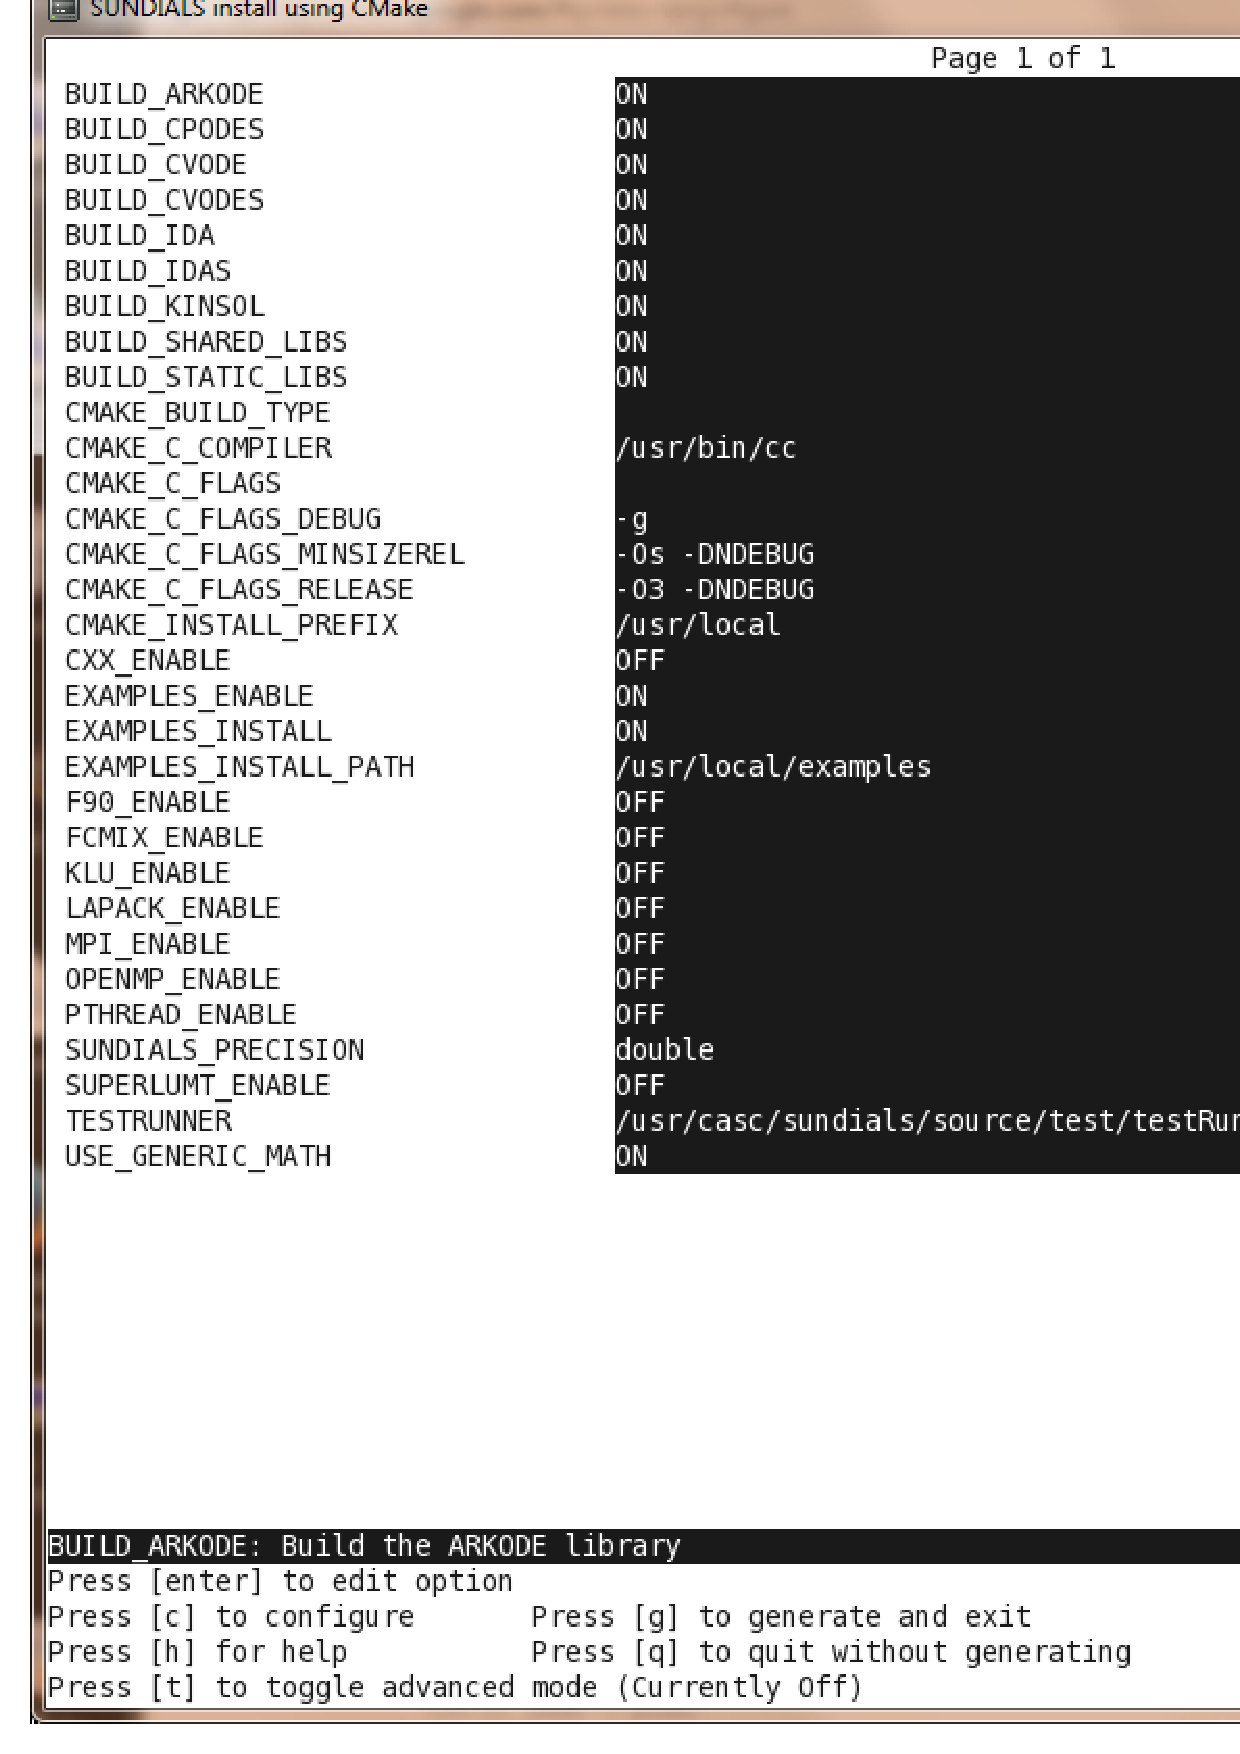
\includegraphics[width=\textwidth]{ccmakedefault}}}
\caption [Initial {\em ccmake} configuration screen]
{Default configuration screen. Note: Initial screen is empty.
To get this default configuration, press 'c' repeatedly (accepting default values denoted with asterisk)
until the 'g' option is available.}
\label{f:ccmakedefault}
\end{figure}

The default {\em instdir} for both {\sundials} and corresponding examples
can be changed by setting the \id{CMAKE\_INSTALL\_PREFIX} and
the \id{EXAMPLES\_INSTALL\_PATH} as shown in figure
\ref{f:ccmakeprefix}. 
\begin{figure}[!ht]
{\centerline{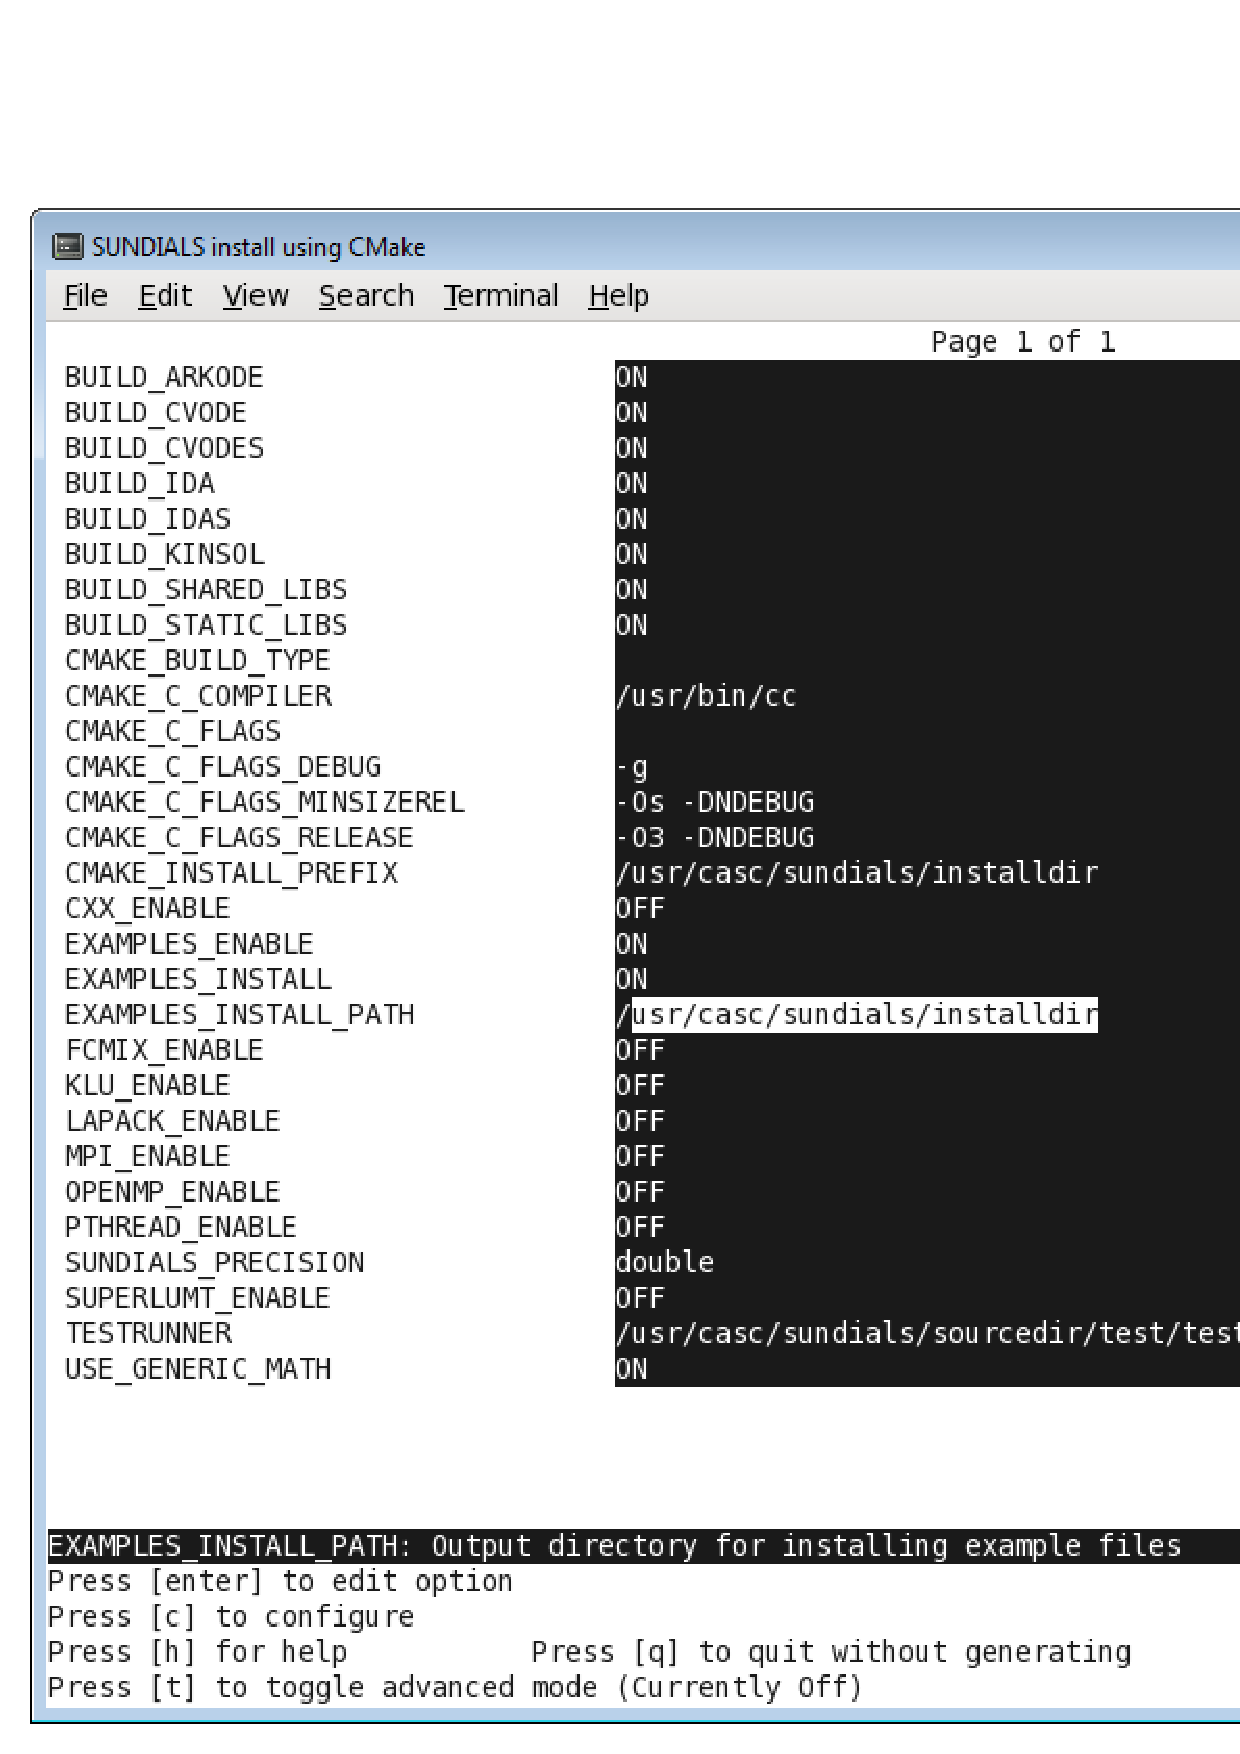
\includegraphics[width=\textwidth]{ccmakeprefix}}}
\caption [Changing the {\em instdir}]
{Changing the {\em instdir} for {\sundials} and
corresponding {\id examples} }
\label{f:ccmakeprefix}
\end{figure}

Pressing the (\id{g} key) will generate makefiles including all dependencies
and all rules to build {\sundials} on this system. 
Back at the command prompt, you can now run:

\begin{verbatim}
  % make
\end{verbatim}

To install {\sundials} in the installation directory specified in the configuration, simply run:

\begin{verbatim}
  % make install
\end{verbatim}

%%
%% *** NOTE: The TestRunner will not be distributed at this time.
%% *** Thus the following is commented out from the documentation.
%% TestRunner
%%
%\subsubsection*{Testing Installation}
%The distribution of {\sundials} includes several examples corresponding to the solvers to be
%installed. Also included in the source bundle is a test script: \id{testRunner}, configured by CMake
%to test the included examples.
%To run the tests, enter:

%\begin{verbatim}
%  % make test
%\end{verbatim}
%The output of \id{testRunner} should look similar to the screens in figure
%\ref{f:testrunner}. The success of each test is based on a line-by-line comparison of expected output files, bundled with the source code, with
%the output of the newly compiled examples. The file compare does allow some differences in rounding for float values.\\\\
%NOTE: Some tests may {\em fail} due to differences in machine architecture, compiler versions, third party libraries etc.{\warn}

%\begin{figure}[!ht]
%{\centerline{\includegraphics{figure=testrunnertop.eps,width=\textwidth}}}
%\vspace{3 mm}
%{\centerline{\includegraphics{figure=testrunnerbot.eps,width=\textwidth}}}
%\caption [Running {\em testRunner}]
%{Invoking {\em testRunner} with {\id make test} to execute all configured
%{\id examples} }
%\label{f:testrunner}
%\end{figure}

 
%%
%% Building from the command line
%%
\subsubsection*{Building from the command line}

Using CMake from the command line is simply a matter of specifying CMake variable settings
with the \id{cmake} command.  The following will build the default configuration:  

\begin{verbatim}
   % cmake -DCMAKE_INSTALL_PREFIX=/home/myname/sundials/instdir \
   > -DEXAMPLES_INSTALL_PATH=/home/myname/sundials/instdir/examples \
   > ../solverdir
   % make
   % make install
\end{verbatim}


\subsection{Configuration options (Unix/Linux)}\label{ss:configuration_options_nix}

A complete list of all available options for a CMake-based {\sundials}
configuration is provide below. Note that the default values shown are for 
a typical configuration on a Linux system and are provided as illustration only.

\begin{description}
\item[\id{BLAS\_ENABLE}] - 
  Enable BLAS support
  \\
  Default: OFF
  \\
  Note: Setting this option to ON will trigger additional CMake
  options. See additional information on building with BLAS enabled
  in \ref{ss:externallibs}.
\item[\id{BLAS\_LIBRARIES}] - 
  BLAS library
  \\
  Default: /usr/lib/libblas.so
  \\
  Note: CMake will search for libraries in your \id{LD\_LIBRARY\_PATH} prior
  to searching default system paths.
\item[\id{BUILD\_ARKODE}] - 
  Build the ARKODE library 
  \\
  Default: ON
\item[\id{BUILD\_CVODE}] - 
  Build the CVODE library 
  \\
  Default: ON
\item[\id{BUILD\_CVODES}] - 
  Build the CVODES library 
  \\
  Default: ON
\item[\id{BUILD\_IDA}] - 
   Build the IDA library 
  \\
   Default: ON
\item[\id{BUILD\_IDAS}] - 
  Build the IDAS library 
  \\
  Default: ON
\item[\id{BUILD\_KINSOL}] - 
  Build the KINSOL library 
  \\
  Default: ON
\item[\id{BUILD\_SHARED\_LIBS}] - 
  Build shared libraries
  \\
  Default: ON
\item[\id{BUILD\_STATIC\_LIBS}] - 
  Build static libraries
  \\
  Default: ON 
\item[\id{CMAKE\_BUILD\_TYPE}] -  
  Choose the type of build, options are: 
  \id{None} (CMAKE\_C\_FLAGS used), \id{Debug}, \id{Release},
  \id{RelWithDebInfo}, and \id{MinSizeRel}
  \\
  Default:
  \\
  Note: Specifying a build type will trigger the corresponding
  build type specific compiler flag options below which will be
  appended to the flags set by
  CMAKE\_{\textless}language{\textgreater}\_FLAGS. 
\item[\id{CMAKE\_C\_COMPILER}] - 
  C compiler
  \\
  Default: /usr/bin/cc 
\item[\id{CMAKE\_C\_FLAGS}] -  
  Flags for C compiler
  \\
  Default:
\item[\id{CMAKE\_C\_FLAGS\_DEBUG}] -      
  Flags used by the C compiler during debug builds
  \\
  Default: -g 
\item[\id{CMAKE\_C\_FLAGS\_MINSIZEREL}] -  
  Flags used by the C compiler during release minsize builds
  \\
  Default: -Os -DNDEBUG 
\item[\id{CMAKE\_C\_FLAGS\_RELEASE}] -    
  Flags used by the C compiler during release builds
  \\
  Default: -O3 -DNDEBUG 
\item[\id{CMAKE\_CXX\_COMPILER}] - 
  {\CPP} compiler
  \\
  Default: /usr/bin/c++
  \\
  Note: A {\CPP} compiler (and all related options) are only
  triggered if {\CPP} examples are enabled (\id{EXAMPLES\_ENABLE\_CXX}
  is ON). All {\sundials} solvers can be used from {\CPP} applications 
  by default without setting any additional configuration options.
\item[\id{CMAKE\_CXX\_FLAGS}] -
  Flags for {\CPP} compiler
  \\
  Default:
\item[\id{CMAKE\_CXX\_FLAGS\_DEBUG}] -
  Flags used by the {\CPP} compiler during debug builds
  \\
  Default: -g 
\item[\id{CMAKE\_CXX\_FLAGS\_MINSIZEREL}] -
  Flags used by the {\CPP} compiler during release minsize builds
  \\
  Default: -Os -DNDEBUG 
\item[\id{CMAKE\_CXX\_FLAGS\_RELEASE}] -
  Flags used by the {\CPP} compiler during release builds
  \\
  Default: -O3 -DNDEBUG
\item[\id{CMAKE\_Fortran\_COMPILER}] - 
  Fortran compiler
  \\
  Default: /usr/bin/gfortran
  \\
  Note: Fortran support (and all related options) are triggered only if
  either Fortran-C support is enabled (\id{FCMIX\_ENABLE} is ON) or
  BLAS/LAPACK support is enabled (\id{BLAS\_ENABLE} or \id{LAPACK\_ENABLE} is ON).
\item[\id{CMAKE\_Fortran\_FLAGS}] - 
  Flags for Fortran compiler
  \\
  Default:
\item[\id{CMAKE\_Fortran\_FLAGS\_DEBUG}] - 
  Flags used by the Fortran compiler during debug builds
  \\
  Default: -g
\item[\id{CMAKE\_Fortran\_FLAGS\_MINSIZEREL}] - 
  Flags used by the Fortran compiler during release minsize builds
  \\
  Default: -Os
\item[\id{CMAKE\_Fortran\_FLAGS\_RELEASE}] - 
  Flags used by the Fortran compiler during release builds
  \\
  Default: -O3
\item[\id{CMAKE\_INSTALL\_PREFIX}] -   
  Install path prefix, prepended onto install directories
  \\
  Default: /usr/local 
  \\
  Note: The user must have write access to the location specified through
  this option. Exported {\sundials} header files and libraries will be 
  installed under subdirectories \id{include} and \id{lib} of 
  \id{CMAKE\_INSTALL\_PREFIX}, respectively.
\item[\id{CUDA\_ENABLE}] -
  Build the {\sundials} {\cuda} vector module.
  \\
  Default: OFF
\item[\id{EXAMPLES\_ENABLE\_C}] -
  Build the {\sundials} {\CC} examples
  \\
  Default: ON
\item[\id{EXAMPLES\_ENABLE\_CUDA}] -
  Build the {\sundials} {\cuda} examples
  \\
  Default: OFF
  \\
  Note: You need to enable {\cuda} support to build these examples.
\item[\id{EXAMPLES\_ENABLE\_CXX}] -
  Build the {\sundials} {\CPP} examples
  \\
  Default: OFF
\item[\id{EXAMPLES\_ENABLE\_RAJA}] -
  Build the {\sundials} {\raja} examples
  \\
  Default: OFF
  \\
  Note: You need to enable {\cuda} and {\raja} support to build these examples.
\item[\id{EXAMPLES\_ENABLE\_F77}] -
  Build the {\sundials} Fortran77 examples
  \\
  Default: ON (if \id{FCMIX\_ENABLE} is ON)
\item[\id{EXAMPLES\_ENABLE\_F90}] -
  Build the {\sundials} Fortran90 examples
  \\
  Default: OFF
\item[\id{EXAMPLES\_INSTALL}] - 
  Install example files
  \\
  Default: ON
  \\
  Note: This option is triggered when any of the {\sundials}
  example programs are enabled \\
  (\id{EXAMPLES\_ENABLE\_$<$language$>$} is ON). If the user requires
  installation of example programs then the sources and sample output files
  for all {\sundials} modules that are currently enabled will be exported to
  the directory specified by \id{EXAMPLES\_INSTALL\_PATH}. A CMake configuration
  script will also be automatically generated and exported to the same directory.
  Additionally, if the configuration is done under a Unix-like system, makefiles
  for the compilation of the example programs (using the installed {\sundials} libraries)
  will be automatically generated and exported to the directory
  specified by \id{EXAMPLES\_INSTALL\_PATH}.
\item[\id{EXAMPLES\_INSTALL\_PATH}] - 
  Output directory for installing example files
  \\
  Default: /usr/local/examples
  \\
  Note: The actual default value for this option will be an \id{examples}
  subdirectory created under \id{CMAKE\_INSTALL\_PREFIX}.
\item[\id{FCMIX\_ENABLE}] - 
  Enable Fortran-C support   
  \\
  Default: OFF 
\item[\id{HYPRE\_ENABLE}] - 
  Enable \textit{hypre} support
  \\
  Default: OFF 
  \\
  Note: See additional information on building with \textit{hypre} enabled in
  \ref{ss:externallibs}. 
\item[\id{HYPRE\_INCLUDE\_DIR}] - 
  Path to \textit{hypre} header files
\item[\id{HYPRE\_LIBRARY\_DIR}] - 
  Path to \textit{hypre} installed library files
\item[\id{KLU\_ENABLE}] - 
  Enable KLU support
  \\
  Default: OFF 
  \\
  Note: See additional information on building with KLU enabled in
  \ref{ss:externallibs}. 
\item[\id{KLU\_INCLUDE\_DIR}] - 
  Path to SuiteSparse header files
\item[\id{KLU\_LIBRARY\_DIR}] - 
  Path to SuiteSparse installed library files
\item[\id{LAPACK\_ENABLE}] -  
  Enable LAPACK support
  \\
  Default: OFF
  \\
  Note: Setting this option to ON will trigger additional CMake
  options. See additional information on building with LAPACK enabled
  in \ref{ss:externallibs}.
\item[\id{LAPACK\_LIBRARIES}] - 
  LAPACK (and BLAS) libraries
  \\
  Default: /usr/lib/liblapack.so;/usr/lib/libblas.so
  \\
  Note: CMake will search for libraries in your \id{LD\_LIBRARY\_PATH} prior
  to searching default system paths.
\item[\id{MPI\_ENABLE}] -
  Enable MPI support (build the parallel nvector).
  \\
  Default: OFF 
  \\
  Note: Setting this option to ON will trigger several additional options
  related to MPI.
\item[\id{MPI\_C\_COMPILER}] -
  \id{mpicc} program
  \\
  Default: 
\item[\id{MPI\_CXX\_COMPILER}] -
  \id{mpicxx} program
  \\
  Default: 
  \\
  Note: This option is triggered only if MPI is enabled
  (\id{MPI\_ENABLE} is ON) and {\CPP} examples are enabled
  (\id{EXAMPLES\_ENABLE\_CXX} is ON). All {\sundials}
  solvers can be used from {\CPP} MPI applications by default
  without setting any additional configuration options other than
  \id{MPI\_ENABLE}.
\item[\id{MPI\_Fortran\_COMPILER}] -
  \id{mpif77} or \id{mpif90} program
  \\
  Default: 
  \\
  Note: This option is triggered only if MPI is enabled
  (\id{MPI\_ENABLE} is ON), Fortran-C support is enabled
  (\id{FCMIX\_ENABLE} is ON), and Fortran77 or Fortran90
  examples are enabled (\id{EXAMPLES\_ENABLE\_F77} or
  \id{EXAMPLES\_ENABLE\_F90} are ON).
\item[\id{MPIEXEC}] -
  Specify the executable for running MPI programs
  \\
  Default: \id{mpirun}
  \\
  Note: This option is triggered only if MPI is enabled
  (\id{MPI\_ENABLE} is ON).
  %% \\
  %% Note: This can either be set to \id{mpirun} for OpenMPI or \id{srun} if jobs are
  %% managed by \id{SLURM} - Simple Linux Utility for Resource Management as exists on
  %% LLNL's high performance computing clusters. 
\item[\id{OPENMP\_ENABLE}] -
  Enable OpenMP support (build the OpenMP nvector).
  \\
  Default: OFF 
\item[\id{PETSC\_ENABLE}] - 
  Enable PETSc support
  \\
  Default: OFF 
  \\
  Note: See additional information on building with PETSc enabled
  in \ref{ss:externallibs}.
\item[\id{PETSC\_INCLUDE\_DIR}] -
  Path to PETSc header files
\item[\id{PETSC\_LIBRARY\_DIR}] - 
  Path to PETSc installed library files
\item[\id{PTHREAD\_ENABLE}] -  
  Enable Pthreads support (build the Pthreads nvector).
  \\
  Default: OFF 
\item[\id{RAJA\_ENABLE}] - 
  Enable {\raja} support (build the {\raja} nvector).
  \\
  Default: OFF 
  \\
  Note: You need to enable {\cuda} in order to build the {\raja} vector module.
\item[\id{SUNDIALS\_F77\_FUNC\_CASE}] - \textbf{advanced option} -
  Specify the case to use in the Fortran name-mangling scheme, options
  are: \id{lower} or \id{upper}
  \\
  Default:
  \\
  Note: The build system will attempt to infer the Fortran
  name-mangling scheme using the Fortran compiler. This option should
  only be used if a Fortran compiler is not available or to override
  the inferred or default (\id{lower}) scheme if one can not be
  determined. If used, \id{SUNDIALS\_F77\_FUNC\_UNDERSCORES} must also
  be set.
\item[\id{SUNDIALS\_F77\_FUNC\_UNDERSCORES}] - \textbf{advanced option} -
  Specify the number of underscores to append in the Fortran
  name-mangling scheme, options are: \id{none}, \id{one}, or \id{two}
  \\
  Default:
  \\
  Note: The build system will attempt to infer the Fortran
  name-mangling scheme using the Fortran compiler. This option should
  only be used if a Fortran compiler is not available or to override
  the inferred or default (\id{one}) scheme if one can not be
  determined. If used, \id{SUNDIALS\_F77\_FUNC\_CASE} must also be set.
\item[\id{SUNDIALS\_INDEX\_TYPE}] - 
  Integer type used for {\sundials} indices, options are: \id{int32\_t} or \id{int64\_t}
  \\
  Default: \id{int64\_t}
\item[\id{SUNDIALS\_PRECISION}] -   
  Precision used in {\sundials}, options are: \id{double}, \id{single}, or \id{extended}
  \\
  Default: \id{double}
\item[\id{SUPERLUMT\_ENABLE}] - 
  Enable SuperLU\_MT support   
  \\
  Default: OFF 
  \\
  Note: See additional information on building with SuperLU\_MT enabled
  in \ref{ss:externallibs}.
\item[\id{SUPERLUMT\_INCLUDE\_DIR}] - 
  Path to SuperLU\_MT header files (typically SRC directory)
\item[\id{SUPERLUMT\_LIBRARY\_DIR}] - 
  Path to SuperLU\_MT installed library files
\item[\id{SUPERLUMT\_THREAD\_TYPE}] - 
  Must be set to Pthread or OpenMP
  \\
  Default: Pthread
\item[\id{USE\_GENERIC\_MATH}] -   
  Use generic (stdc) math libraries
  \\
  Default: ON 
\end{description}

\subsubsection*{xSDK Configuration Options}

{\sundials} supports CMake configuration options defined by the
Extreme-scale Scientific Software Development Kit (xSDK) community
policies (see {\tt https://xsdk.info} for more information). xSDK
CMake options are unused by default but may be activated by setting
\id{USE\_XSDK\_DEFAULTS} to ON.

{\warn} When xSDK options are active, they will overwrite the
corresponding {\sundials} option and may have different default values
(see details below). As such the equivalent {\sundials} options should
not be used when configuring with xSDK options. In the GUI front end
to CMake (\id{ccmake}), setting \id{USE\_XSDK\_DEFAULTS} to ON will
hide the corresponding {\sundials} options as advanced CMake variables.
During configuration, messages are output detailing
which xSDK flags are active and the equivalent {\sundials} options
that are replaced. Below is a complete list xSDK options and the
corresponding {\sundials} options if applicable.

\begin{description}
\item[\id{TPL\_BLAS\_LIBRARIES}] - 
  BLAS library
  \\
  Default: /usr/lib/libblas.so
  \\
  {\sundials} equivalent: \id{BLAS\_LIBRARIES}
  \\
  Note: CMake will search for libraries in your \id{LD\_LIBRARY\_PATH} prior
  to searching default system paths.
\item[\id{TPL\_ENABLE\_BLAS}] - 
  Enable BLAS support
  \\
  Default: OFF
  \\
  {\sundials} equivalent: \id{BLAS\_ENABLE}
\item[\id{TPL\_ENABLE\_HYPRE}] - 
  Enable \textit{hypre} support
  \\
  Default: OFF
  \\
  {\sundials} equivalent: \id{HYPRE\_ENABLE}
\item[\id{TPL\_ENABLE\_KLU}] - 
  Enable KLU support
  \\
  Default: OFF
  \\
  {\sundials} equivalent: \id{KLU\_ENABLE}
\item[\id{TPL\_ENABLE\_PETSC}] - 
  Enable PETSc support
  \\
  Default: OFF
  \\
  {\sundials} equivalent: \id{PETSC\_ENABLE}
\item[\id{TPL\_ENABLE\_LAPACK}] - 
  Enable LAPACK support
  \\
  Default: OFF
  \\
  {\sundials} equivalent: \id{LAPACK\_ENABLE}
\item[\id{TPL\_ENABLE\_SUPERLUMT}] - 
  Enable SuperLU\_MT support
  \\
  Default: OFF
  \\
  {\sundials} equivalent: \id{SUPERLUMT\_ENABLE}
\item[\id{TPL\_HYPRE\_INCLUDE\_DIRS}] - 
  Path to \textit{hypre} header files
  \\
  {\sundials} equivalent: \id{HYPRE\_INCLUDE\_DIR}
\item[\id{TPL\_HYPRE\_LIBRARIES}] - 
  \textit{hypre} library
  \\
  {\sundials} equivalent: N/A
\item[\id{TPL\_KLU\_INCLUDE\_DIRS}] - 
  Path to KLU header files
  \\
  {\sundials} equivalent: \id{KLU\_INCLUDE\_DIR}
\item[\id{TPL\_KLU\_LIBRARIES}] - 
  KLU library
  \\
  {\sundials} equivalent: N/A
\item[\id{TPL\_LAPACK\_LIBRARIES}] - 
  LAPACK (and BLAS) libraries
  \\
  Default: /usr/lib/liblapack.so;/usr/lib/libblas.so
  \\
  {\sundials} equivalent: \id{LAPACK\_LIBRARIES}
  \\
  Note: CMake will search for libraries in your \id{LD\_LIBRARY\_PATH} prior
  to searching default system paths.
\item[\id{TPL\_PETSC\_INCLUDE\_DIRS}] - 
  Path to PETSc header files
  \\
  {\sundials} equivalent: \id{PETSC\_INCLUDE\_DIR}
\item[\id{TPL\_PETSC\_LIBRARIES}] - 
  PETSc library
  \\
  {\sundials} equivalent: N/A
\item[\id{TPL\_SUPERLUMT\_INCLUDE\_DIRS}] - 
  Path to SuperLU\_MT header files
  \\
  {\sundials} equivalent: \id{SUPERLUMT\_INCLUDE\_DIR}
\item[\id{TPL\_SUPERLUMT\_LIBRARIES}] - 
  SuperLU\_MT library
  \\
  {\sundials} equivalent: N/A
\item[\id{TPL\_SUPERLUMT\_THREAD\_TYPE}] - 
  SuperLU\_MT library thread type
  \\
  {\sundials} equivalent: \id{SUPERLUMT\_THREAD\_TYPE}
\item[\id{USE\_XSDK\_DEFAULTS}] - 
  Enable xSDK default configuration settings
  \\
  Default: OFF
  \\
  {\sundials} equivalent: N/A
  \\
  Note: Enabling xSDK defaults also sets \id{CMAKE\_BUILD\_TYPE} to \id{Debug}
\item[\id{XSDK\_ENABLE\_FORTRAN}] -
  Enable {\sundials} Fortran interface
  \\
  Default: OFF
  \\
  {\sundials} equivalent: \id{FCMIX\_ENABLE}
\item[\id{XSDK\_INDEX\_SIZE}] -
  Integer size (bits) used for indices in {\sundials}, options are: \id{32} or \id{64}
  \\
  Default: \id{32}
  \\
  {\sundials} equivalent: \id{SUNDIALS\_INDEX\_TYPE}
\item[\id{XSDK\_PRECISION}] -
  Precision used in {\sundials}, options are: \id{double}, \id{single}, or \id{quad}
  \\
  Default: \id{double}
  \\
  {\sundials} equivalent: \id{SUNDIALS\_PRECISION}
\end{description}



%%===============================================================================

\subsection{Configuration examples}

The following examples will help demonstrate usage of the CMake configure options.

\noindent To configure {\sundials} using the default C and Fortran compilers,
and default \id{mpicc} and \id{mpif77} parallel compilers, 
enable compilation of examples, and install libraries, headers, and
example sources under subdirectories of
\id{/home/myname/sundials/}, use:

\begin{verbatim}
   % cmake \
   > -DCMAKE_INSTALL_PREFIX=/home/myname/sundials/instdir \
   > -DEXAMPLES_INSTALL_PATH=/home/myname/sundials/instdir/examples \
   > -DMPI_ENABLE=ON \
   > -DFCMIX_ENABLE=ON \
   > /home/myname/sundials/solverdir
   %
   % make install
   % 
\end{verbatim}

\noindent To disable installation of the examples, use:
\begin{verbatim}
   % cmake \
   > -DCMAKE_INSTALL_PREFIX=/home/myname/sundials/instdir \
   > -DEXAMPLES_INSTALL_PATH=/home/myname/sundials/instdir/examples \
   > -DMPI_ENABLE=ON \
   > -DFCMIX_ENABLE=ON \
   > -DEXAMPLES_INSTALL=OFF \
   > /home/myname/sundials/solverdir
   %
   % make install
   % 
\end{verbatim}

%%===============================================================================
\subsection{Working with external Libraries} \label{ss:externallibs}

The {\sundials} suite contains many options to enable implementation flexibility
when developing solutions. The following are some notes addressing specific configurations
when using the supported third party libraries.
When building {\sundials} as a shared library external libraries any
used with {\sundials} must also be build as a shared library or as a
static library compiled with the \id{-fPIC} flag.{\warn}

\subsubsection*{Building with BLAS}
{\sundials} does not utilize BLAS directly but it may be needed by other
external libraries that {\sundials} can be built with (e.g. LAPACK,
PETSc, SuperLU\_MT, etc.). To enable BLAS, set the \id{BLAS\_ENABLE}
option to \id{ON}. If the directory containing the BLAS library is in
the \id{LD\_LIBRARY\_PATH} environment variable, CMake will set the
\id{BLAS\_LIBRARIES} variable accordingly, otherwise CMake will
attempt to find the BLAS library in standard system locations. To
explicitly tell CMake what libraries to use, the \id{BLAS\_LIBRARIES}
variable can be set to the desired library. Example:
\begin{verbatim}
   % cmake \
   > -DCMAKE_INSTALL_PREFIX=/home/myname/sundials/instdir \
   > -DEXAMPLES_INSTALL_PATH=/home/myname/sundials/instdir/examples \
   > -DBLAS_ENABLE=ON \
   > -DBLAS_LIBRARIES=/myblaspath/lib/libblas.so \
   > -DSUPERLUMT_ENABLE=ON \
   > -DSUPERLUMT_INCLUDE_DIR=/mysuperlumtpath/SRC
   > -DSUPERLUMT_LIBRARY_DIR=/mysuperlumtpath/lib
   > /home/myname/sundials/solverdir
   %
   % make install
   % 
\end{verbatim}
{\warn}When allowing CMake to automatically locate the LAPACK library,
CMake \textit{may} also locate the corresponding BLAS library.

If a working Fortran compiler is not available to infer the Fortran
name-mangling scheme, the options \id{SUNDIALS\_F77\_FUNC\_CASE} and
\id{SUNDIALS\_F77\_FUNC\_UNDERSCORES} \textit{must} be set in order to
bypass the check for a Fortran compiler and define the name-mangling
scheme. The defaults for these options in earlier versions of
{\sundials} were \id{lower} and \id{one} respectively.


\subsubsection*{Building with LAPACK}
To enable LAPACK, set the \id{LAPACK\_ENABLE} option to \id{ON}.
If the directory containing the LAPACK library is in the
\id{LD\_LIBRARY\_PATH} environment variable, CMake will set the
\id{LAPACK\_LIBRARIES} variable accordingly, otherwise CMake will
attempt to find the LAPACK library in standard system locations. To
explicitly tell CMake what library to use, the \id{LAPACK\_LIBRARIES}
variable can be set to the desired libraries. {\warn}When setting
the LAPACK location explicitly the location of the corresponding BLAS
library will also need to be set. Example:
\begin{verbatim}
   % cmake \
   > -DCMAKE_INSTALL_PREFIX=/home/myname/sundials/instdir \
   > -DEXAMPLES_INSTALL_PATH=/home/myname/sundials/instdir/examples \
   > -DBLAS_ENABLE=ON \
   > -DBLAS_LIBRARIES=/mylapackpath/lib/libblas.so \
   > -DLAPACK_ENABLE=ON \
   > -DLAPACK_LIBRARIES=/mylapackpath/lib/liblapack.so \
   > /home/myname/sundials/solverdir
   %
   % make install
   % 
\end{verbatim}
{\warn}When allowing CMake to automatically locate the LAPACK library,
CMake \textit{may} also locate the corresponding BLAS library.

If a working Fortran compiler is not available to infer the Fortran
name-mangling scheme, the options \id{SUNDIALS\_F77\_FUNC\_CASE} and
\id{SUNDIALS\_F77\_FUNC\_UNDERSCORES} \textit{must} be set in order to
bypass the check for a Fortran compiler and define the name-mangling
scheme. The defaults for these options in earlier versions of
{\sundials} were \id{lower} and \id{one} respectively.

\subsubsection*{Building with KLU}
The KLU libraries are part of SuiteSparse, a suite of sparse matrix software,
available from the Texas A\&M University website: {\tt http://faculty.cse.tamu.edu/davis/suitesparse.html}.
{\sundials} has been tested with SuiteSparse version 4.5.3.
To enable KLU, set \id{KLU\_ENABLE} to \id{ON}, set \id{KLU\_INCLUDE\_DIR} to the \id{include}
path of the KLU installation and set \id{KLU\_LIBRARY\_DIR} to the \id{lib} path of the KLU installation.
The CMake configure will result in populating the following variables: \id{AMD\_LIBRARY},
\id{AMD\_LIBRARY\_DIR}, \id{BTF\_LIBRARY}, \id{BTF\_LIBRARY\_DIR},
\id{COLAMD\_LIBRARY}, \id{COLAMD\_LIBRARY\_DIR}, and
\newline\id{KLU\_LIBRARY}.

\subsubsection*{Building with SuperLU\_MT}
The SuperLU\_MT libraries are available for download from the Lawrence Berkeley National Laboratory website:
{\tt http://crd-legacy.lbl.gov/$\sim$xiaoye/SuperLU/\#superlu\_mt}. 
{\sundials} has been tested with SuperLU\_MT version 3.1. 
To enable SuperLU\_MT, set  \id{SUPERLUMT\_ENABLE} to \id{ON}, set \id{SUPERLUMT\_INCLUDE\_DIR}
to the \id{SRC} path of the SuperLU\_MT installation, and set the variable
\newline\id{SUPERLUMT\_LIBRARY\_DIR} to the \id{lib} path of the SuperLU\_MT installation.
At the same time, the variable
\id{SUPERLUMT\_THREAD\_TYPE} must be set to either \id{Pthread} or \id{OpenMP}.

\noindent Do not mix thread types when building {\sundials} solvers.
If threading is enabled for {\sundials} by having either \id{OPENMP\_ENABLE} or \id{PTHREAD\_ENABLE} set to \id{ON}
then SuperLU\_MT should be set to use the same threading type.{\warn}

\subsubsection*{Building with PETSc}
The PETSc libraries are available for download from the Argonne National Laboratory website:
{\tt http://www.mcs.anl.gov/petsc}. 
{\sundials} has been tested with PETSc version 3.7.2. 
To enable PETSc, set  \id{PETSC\_ENABLE} to \id{ON}, set \id{PETSC\_INCLUDE\_DIR}
to the \id{include} path of the PETSc installation, and set the variable
\id{PETSC\_LIBRARY\_DIR} to the \id{lib} path of the PETSc installation.


\subsubsection*{Building with \textit{hypre}}
The \textit{hypre} libraries are available for download from the Lawrence Livermore
National Laboratory website: {\tt http://computation.llnl.gov/projects/hypre}.
%{\tt http://computation.llnl.gov/projects/hypre-scalable-linear-solvers-multigrid-methods}.
{\sundials} has been tested with \textit{hypre} version 2.11.1. 
To enable \textit{hypre}, set  \id{HYPRE\_ENABLE} to \id{ON}, set \id{HYPRE\_INCLUDE\_DIR}
to the \id{include} path of the \textit{hypre} installation, and set the variable
\id{HYPRE\_LIBRARY\_DIR} to the \id{lib} path of the \textit{hypre} installation.

\subsubsection*{Building with CUDA}
{\sundials} {\cuda} modules and examples have been tested with version 8.0 of the 
{\cuda} toolkit. To build them, you need to install the Toolkit and compatible
NVIDIA drivers. Both are available for download from the NVIDIA website:
{\tt https://developer.nvidia.com/cuda-downloads}. To enable {\cuda}, 
set \id{CUDA\_ENABLE} to \id{ON}. If {\cuda} is installed in a
nonstandard location, you may be prompted to set the variable
\id{CUDA\_TOOLKIT\_ROOT\_DIR} with your {\cuda} Toolkit installation
path. To enable {\cuda} examples, set \id{EXAMPLES\_ENABLE\_CUDA} to \id{ON}.

\subsubsection*{Building with RAJA}
{\raja} is a performance portability layer developed by Lawrence
Livermore National Laboratory and can be obtained from {\tt https://github.com/LLNL/RAJA}.
{\sundials} {\raja} modules and examples have been tested with {\raja}
version 0.3. Building {\sundials} {\raja} modules requires a
{\cuda}-enabled {\raja} installation. To enable {\raja}, set
\id{CUDA\_ENABLE} and \id{RAJA\_ENABLE} to \id{ON}. If {\raja} is
installed in a nonstandard location you will be prompted to set the
variable \id{RAJA\_DIR} with the path to the {\raja} CMake
configuration file. To enable building the {\raja} examples set
\id{EXAMPLES\_ENABLE\_RAJA} to \id{ON}.

\subsection{Testing the build and installation}

If {\sundials} was configured with
\id{EXAMPLES\_ENABLE\_$<$language$>$} options to \id{ON}, then a set of
regression tests can be run after building with the \id{make} command
by running: 
\begin{verbatim}
  % make test
\end{verbatim}
Additionally, if \id{EXAMPLES\_INSTALL} was also set to \id{ON}, then
a set of smoke tests can be run after installing with the \id{make install} 
command by running:
\begin{verbatim}
  % make test_install
\end{verbatim}

%%===============================================================================
\section{Building and Running Examples}
%%===============================================================================
Each of the {\sundials} solvers is distributed with a set of examples
demonstrating basic usage. To build and install the examples, set at
least of the \id{EXAMPLES\_ENABLE\_$<$language$>$} options to \id{ON}, and
set \id{EXAMPLES\_INSTALL} to \id{ON}.
Specify the installation path for the examples with the variable \id{EXAMPLES\_INSTALL\_PATH}. CMake will generate
\id{CMakeLists.txt} configuration files (and \id{Makefile} files if on Linux/Unix) that reference the
{\em installed} {\sundials} headers and libraries.

Either the \id{CMakeLists.txt} file or the traditional \id{Makefile} may be used to build the examples
as well as serve as a template for creating user developed solutions.
To use the supplied \id{Makefile} simply run \id{make} to compile and generate the executables.
To use CMake from within the installed example directory, run \id{cmake} (or \id{ccmake} to use the GUI)
followed by \id{make} to compile the example code.
Note that if CMake is used, it will overwrite the traditional \id{Makefile} with a new CMake-generated \id{Makefile}.
The resulting output from running the examples can be compared with example output bundled
in the {\sundials} distribution.

\noindent NOTE: There will potentially be differences in the output due to machine architecture, compiler versions,
use of third party libraries etc.{\warn} 


%%===============================================================================
\section{Configuring, building, and installing  on Windows}\label{s:cmake_windows}
%%===============================================================================
CMake can also be used to build {\sundials} on Windows. To build {\sundials} for
use with Visual Studio the following steps should be performed:
\begin{enumerate}
\item Unzip the downloaded tar file(s) into a directory. This will be the {\em solverdir} 
\item Create a separate {\em builddir}
\item Open a Visual Studio Command Prompt and cd to {\em builddir}
\item Run cmake-gui ../{\em solverdir}
\begin{enumerate}
\item Hit Configure
\item Check/Uncheck solvers to be built
\item Change CMAKE\_INSTALL\_PREFIX to {\em instdir}
\item Set other options as desired
\item Hit Generate
\end{enumerate}
\item Back in the VS Command Window:
\begin{enumerate}
\item Run msbuild ALL\_BUILD.vcxproj
\item Run msbuild INSTALL.vcxproj
\end{enumerate} 
\end{enumerate}

\noindent The resulting libraries will be in the {\em instdir}.
\noindent The {\sundials} project can also now be opened in Visual Studio.
Double click on the ALL\_BUILD.vcxproj file to open the project.
Build the whole {\em solution} to create the {\sundials} libraries.
To use the {\sundials} libraries in your own projects, you must
set the include directories for your project,
add the {\sundials} libraries to your project solution,
and set the {\sundials} libraries as dependencies for your project.

%%===============================================================================
\section{Installed libraries and exported header files}
%%===============================================================================

Using the CMake {\sundials} build system, the command
\begin{verbatim}
   % make install
\end{verbatim}
will install the libraries under {\em libdir} and the public header
files under {\em includedir}. The values for these directories are
{\em instdir}\id{/lib} and {\em instdir}\id{/include},
respectively. The location can be changed by setting the CMake variable \id{CMAKE\_INSTALL\_PREFIX}.
Although all installed libraries reside under {\em libdir}\id{/lib}, the public header files
are further organized into subdirectories under {\em includedir}\id{/include}.

The installed libraries and exported header files are listed for
reference in Table \ref{t:sundials_files}.
The file extension .{\em lib}
is typically \id{.so} for shared libraries and \id{.a} for static libraries.
Note that, in the Tables, names are relative to {\em libdir}
for libraries and to {\em includedir} for header files.

A typical user program need not explicitly include any of the shared
{\sundials} header files from under the {\em includedir}\id{/include}\id{/sundials}
directory since they are explicitly included by the appropriate solver
header files ({\em e.g.}, \id{cvode\_dense.h} includes
\id{sundials\_dense.h}). However, it is both legal and safe to do so,
and would be useful, for example, if the functions declared in \id{sundials\_dense.h} 
are to be used in building a preconditioner.

%---------------------------------------------------------------------------
% Table of installed files
%---------------------------------------------------------------------------

\newlength{\colLenOne}
\settowidth{\colLenOne}{{\sunlinsollapdense}}

\newlength{\colLenTwo}
\settowidth{\colLenTwo}{Header files}

\newlength{\colLenThree}
\setlength{\colLenThree}{\textwidth}
\addtolength{\colLenThree}{-0.5in}
\addtolength{\colLenThree}{-\colLenOne}
\addtolength{\colLenThree}{-\colLenTwo}

%\caption{{\sundials} libraries and header files (cont.)}\label{t:sundials_files2}

\tablecaption{{\sundials} libraries and header files}\label{t:sundials_files}
\tablefirsthead{\hline}
\tablehead{\hline \multicolumn{4}{|l|}{\small\slshape continued from last page} \\
           \hline}
\tabletail{\hline \multicolumn{4}{|r|}{\small\slshape continued on next page} \\ \hline}
\begin{xtabular}{|p{\colLenOne}|p{\colLenTwo}|p{0.5\colLenThree} p{0.5\colLenThree}|}

%% --------------------------------------------------
{\shared}
 & Libraries    & n/a  & \\
\cline{2-4}
 & Header files & sundials/sundials\_config.h        & sundials/sundials\_fconfig.h  \\
 &              & sundials/sundials\_types.h         & sundials/sundials\_math.h     \\
 &              & sundials/sundials\_nvector.h       & sundials/sundials\_fnvector.h \\
 &              & sundials/sundials\_iterative.h     & sundials/sundials\_direct.h   \\
 &              & sundials/sundials\_dense.h         & sundials/sundials\_band.h     \\
 &              & sundials/sundials\_matrix.h        & sundials/sundials\_version.h  \\
 &              & sundials/sundials\_linearsolver.h  & \\
\hline
%% --------------------------------------------------
{\nvecs}
 & Libraries    & libsundials\_nvecserial.{\em lib} & libsundials\_fnvecserial.a \\ 
\cline{2-4}
 & Header files & nvector/nvector\_serial.h         & \\ 
\hline
%% --------------------------------------------------
{\nvecp}
 & Libraries    & libsundials\_nvecparallel.{\em lib} & libsundials\_fnvecparallel.a \\
\cline{2-4}
 & Header files & nvector/nvector\_parallel.h         & \\
\hline
%% --------------------------------------------------
{\nvecopenmp}
 & Libraries    & libsundials\_nvecopenmp.{\em lib} & libsundials\_fnvecopenmp.a \\ 
\cline{2-4}
 & Header files & nvector/nvector\_openmp.h         & \\ 
\hline
%% --------------------------------------------------
{\nvecpthreads}
 & Libraries    & libsundials\_nvecpthreads.{\em lib} & libsundials\_fnvecpthreads.a \\ 
\cline{2-4}
 & Header files & nvector/nvector\_pthreads.h         & \\ 
\hline
%% --------------------------------------------------
{\nvecph}
 & Libraries    & libsundials\_nvecparhyp.{\em lib} & \\
\cline{2-4}
 & Header files & nvector/nvector\_parhyp.h         & \\ 
\hline
%% --------------------------------------------------
{\nvecpetsc}
 & Libraries    & libsundials\_nvecpetsc.{\em lib} & \\ 
\cline{2-4}
 & Header files & nvector/nvector\_petsc.h         & \\ 
\hline
%% --------------------------------------------------
{\nveccuda}
 & Libraries    & libsundials\_nveccuda.{\em lib}     & \\ 
\cline{2-4}
 & Header files & nvector/nvector\_cuda.h             & \\
 &              & nvector/cuda/ThreadPartitioning.hpp & \\
 &              & nvector/cuda/Vector.hpp             & \\
 &              & nvector/cuda/VectorKernels.cuh      & \\
\hline
%% --------------------------------------------------
{\nvecraja}
 & Libraries    & libsundials\_nvecraja.{\em lib} & \\ 
\cline{2-4}
 & Header files & nvector/nvector\_raja.h         & \\
 &              & nvector/raja/Vector.hpp         & \\
\hline
%% --------------------------------------------------
{\sunmatband}
 & Libraries    & libsundials\_sunmatrixband.{\em lib} & \\ 
 &              & libsundials\_fsunmatrixband.a        & \\ 
\cline{2-4}
 & Header files & sunmatrix/sunmatrix\_band.h          & \\ 
\hline
%% --------------------------------------------------
{\sunmatdense}
 & Libraries    & libsundials\_sunmatrixdense.{\em lib} & \\
 &              & libsundials\_fsunmatrixdense.a        & \\
\cline{2-4}
 & Header files & sunmatrix/sunmatrix\_dense.h          & \\
\hline
%% --------------------------------------------------
{\sunmatsparse}
 & Libraries    & libsundials\_sunmatrixsparse.{\em lib} & \\ 
 &              & libsundials\_fsunmatrixsparse.a        & \\ 
\cline{2-4}
 & Header files & sunmatrix/sunmatrix\_sparse.h          & \\ 
\hline
%% --------------------------------------------------
{\sunlinsolband}
 & Libraries    & libsundials\_sunlinsolband.{\em lib} & \\ 
 &              & libsundials\_fsunlinsolband.a        & \\ 
\cline{2-4}
 & Header files & sunlinsol/sunlinsol\_band.h          & \\ 
\hline
%% --------------------------------------------------
{\sunlinsoldense}
 & Libraries    & libsundials\_sunlinsoldense.{\em lib} & \\ 
 &              & libsundials\_fsunlinsoldense.a        & \\ 
\cline{2-4}
 & Header files & sunlinsol/sunlinsol\_dense.h          & \\ 
\hline
%% --------------------------------------------------
{\sunlinsolklu}
 & Libraries    & libsundials\_sunlinsolklu.{\em lib} & \\ 
 &              & libsundials\_fsunlinsolklu.a        & \\ 
\cline{2-4}
 & Header files & sunlinsol/sunlinsol\_klu.h          & \\ 
\hline
%% --------------------------------------------------
{\sunlinsollapband}
 & Libraries    & libsundials\_sunlinsollapackband.{\em lib} & \\ 
 &              & libsundials\_fsunlinsollapackband.a        & \\ 
\cline{2-4}
 & Header files & sunlinsol/sunlinsol\_lapackband.h          & \\ 
\hline
%% --------------------------------------------------
{\sunlinsollapdense}
 & Libraries    & libsundials\_sunlinsollapackdense.{\em lib} & \\ 
 &              & libsundials\_fsunlinsollapackdense.a        & \\ 
\cline{2-4}
 & Header files & sunlinsol/sunlinsol\_lapackdense.h          & \\ 
\hline
%% --------------------------------------------------
{\sunlinsolpcg}
 & Libraries    & libsundials\_sunlinsolpcg.{\em lib} & \\ 
 &              & libsundials\_fsunlinsolpcg.a        & \\ 
\cline{2-4}
 & Header files & sunlinsol/sunlinsol\_pcg.h          & \\ 
\hline
%% --------------------------------------------------
{\sunlinsolspbcgs}
 & Libraries    & libsundials\_sunlinsolspbcgs.{\em lib} & \\ 
 &              & libsundials\_fsunlinsolspbcgs.a        & \\ 
\cline{2-4}
 & Header files & sunlinsol/sunlinsol\_spbcgs.h          & \\ 
\hline
%% --------------------------------------------------
{\sunlinsolspfgmr}
 & Libraries    & libsundials\_sunlinsolspfgmr.{\em lib} & \\ 
 &              & libsundials\_fsunlinsolspfgmr.a        & \\ 
\cline{2-4}
 & Header files & sunlinsol/sunlinsol\_spfgmr.h          & \\ 
\hline
%% --------------------------------------------------
{\sunlinsolspgmr}
 & Libraries    & libsundials\_sunlinsolspgmr.{\em lib} & \\ 
 &              & libsundials\_fsunlinsolspgmr.a        & \\ 
\cline{2-4}
 & Header files & sunlinsol/sunlinsol\_spgmr.h          & \\ 
\hline
%% --------------------------------------------------
{\sunlinsolsptfqmr}
 & Libraries    & libsundials\_sunlinsolsptfqmr.{\em lib} & \\ 
 &              & libsundials\_fsunlinsolsptfqmr.a        & \\ 
\cline{2-4}
 & Header files & sunlinsol/sunlinsol\_sptfqmr.h          & \\ 
\hline
%% --------------------------------------------------
{\sunlinsolslumt}
 & Libraries    & libsundials\_sunlinsolsuperlumt.{\em lib} & \\ 
 &              & libsundials\_fsunlinsolsuperlumt.a        & \\ 
\cline{2-4}
 & Header files & sunlinsol/sunlinsol\_superlumt.h          & \\ 
\hline
%% --------------------------------------------------
{\cvode}
 & Libraries    & libsundials\_cvode.{\em lib} & libsundials\_fcvode.a \\
\cline{2-4}
 & Header files & cvode/cvode.h                & cvode/cvode\_impl.h   \\
 &              & cvode/cvode\_direct.h        & cvode/cvode\_spils.h  \\
 &              & cvode/cvode\_bandpre.h       & cvode/cvode\_bbdpre.h \\
\hline
%% --------------------------------------------------
{\cvodes}
 & Libraries    & libsundials\_cvodes.{\em lib} & \\
\cline{2-4}
 & Header files & cvodes/cvodes.h               & cvodes/cvodes\_impl.h   \\
 &              & cvodes/cvodes\_direct.h       & cvodes/cvodes\_spils.h  \\
 &              & cvodes/cvodes\_bandpre.h      & cvodes/cvodes\_bbdpre.h \\
\hline
%% --------------------------------------------------
{\arkode}
 & Libraries    & libsundials\_arkode.{\em lib} & libsundials\_farkode.a \\
\cline{2-4}
 & Header files & arkode/arkode.h               & arkode/arkode\_impl.h   \\
 &              & arkode/arkode\_direct.h       & arkode/arkode\_spils.h  \\
 &              & arkode/arkode\_bandpre.h      & arkode/arkode\_bbdpre.h \\
\hline
%% --------------------------------------------------
{\ida}
 & Libraries    & libsundials\_ida.{\em lib} & libsundials\_fida.a \\
\cline{2-4}
 & Header files & ida/ida.h                  & ida/ida\_impl.h     \\
 &              & ida/ida\_direct.h          & ida/ida\_spils.h    \\
 &              & ida/ida\_bbdpre.h          & \\
\hline
%% --------------------------------------------------
{\idas}
 & Libraries    & libsundials\_idas.{\em lib} & \\
\cline{2-4}
 & Header files & idas/idas.h                 & idas/idas\_impl.h     \\
 &              & idas/idas\_direct.h         & idas/idas\_spils.h    \\
 &              & idas/idas\_bbdpre.h         & \\
\hline 
%% --------------------------------------------------
{\kinsol}
 & Libraries    & libsundials\_kinsol.{\em lib} & libsundials\_fkinsol.a \\
\cline{2-4}
 & Header files & kinsol/kinsol.h               & kinsol/kinsol\_impl.h     \\
 &              & kinsol/kinsol\_direct.h       & kinsol/kinsol\_spils.h    \\
 &              & kinsol/kinsol\_bbdpre.h       & \\
\hline
 %% --------------------------------------------------
\end{xtabular}

\clearemptydoublepage
%===============================================================
% KINSOL constants
L%%========================================================================
\chapter{KINSOL Constants}\label{c:constants}
%%========================================================================

Below we list all input and output constants used by the main solver and 
linear solver modules, together with their numerical values and a short
description of their meaning.

%%-------------------------------------------------------------------------
%% Supertabular setings

\newlength{\tcolone}
\settowidth{\tcolone}{\id{SPTFQMR\_PSOLVE\_FAIL\_UNREC}}
\newlength{\tcoltwo}
\settowidth{\tcoltwo}{-20}
\newlength{\tcolthree}
\setlength{\tcolthree}{\textwidth}
\addtolength{\tcolthree}{-0.5in}
\addtolength{\tcolthree}{-\tcolone}
\addtolength{\tcolthree}{-\tcoltwo}

\tablefirsthead{}
\tablehead{}
\tabletail{}
\tablelasttail{}

%%-------------------------------------------------------------------------

\section{KINSOL input constants}\label{s:kinsol_in_constants}

\begin{supertabular*}{\textwidth}{p{\tcolone}@{\hspace*{2mm}\extracolsep{\fill}}rp{\tcolthree}}

\hline
\multicolumn{3}{c}{\bf {\kinsol} main solver module}\\
\hline\\

\id{KIN\_ETACHOICE1}      & 1 & Use Eisenstat and Walker Choice 1 for $\eta$. \\
\id{KIN\_ETACHOICE2}      & 2 & Use Eisenstat and Walker Choice 2 for $\eta$. \\
\id{KIN\_ETACONSTANT}     & 3 & Use constant value for $\eta$. \\
\id{KIN\_NONE}            & 0 & Use inexact Newton globalization. \\
\id{KIN\_LINESEARCH}      & 1 & Use linesearch globalization.

\\\hline
\multicolumn{3}{c}{\bf Iterative linear solver module}\\
\hline\\

\id{PREC\_NONE}    & 0 & No preconditioning \\
\id{PREC\_RIGHT}   & 2 & Preconditioning on the right. \\
\id{MODIFIED\_GS}  & 1 & Use modified Gram-Schmidt procedure. \\
\id{CLASSICAL\_GS} & 2 & Use classical Gram-Schmidt procedure. \\

\end{supertabular*}

%%-------------------------------------------------------------------------

\section{KINSOL output constants}\label{s:kinsol_out_constants}

\begin{supertabular*}{\textwidth}{p{\tcolone}@{\hspace*{2mm}\extracolsep{\fill}}rp{\tcolthree}}

\hline
\multicolumn{3}{c}{\bf {\kinsol} main solver module}\\
\hline\\

\id{KIN\_SUCCESS}               &  0  & Successful function return. \\
\id{KIN\_INITIAL\_GUESS\_OK}    &  1  & The initial user-supplied guess already satisfies the stopping criterion. \\
\id{KIN\_STEP\_LT\_STPTOL}      &  2  & The stopping tolerance on scaled step length was satisfied. \\
\id{KIN\_WARNING}               & 99  & A non-fatal warning. The solver will continue. \\
\id{KIN\_MEM\_NULL}             & -1  & The \id{kin\_mem} argument was \id{NULL}. \\
\id{KIN\_ILL\_INPUT}            & -2  & One of the function inputs is illegal. \\
\id{KIN\_NO\_MALLOC}            & -3  & The {\kinsol} memory was not allocated by a call to \id{KINMalloc}. \\
\id{KIN\_MEM\_FAIL}             & -4  & A memory allocation failed. \\
\id{KIN\_LINESEARCH\_NONCONV}   & -5  & The linesearch algorithm was unable to find an iterate sufficiently distinct from the current iterate. \\
\id{KIN\_MAXITER\_REACHED}      & -6  & The maximum number of nonlinear iterations has been reached. \\
\id{KIN\_MXNEWT\_5X\_EXCEEDED}  & -7  & Five consecutive steps have been taken that satisfy a scaled step length test. \\
\id{KIN\_LINESEARCH\_BCFAIL}    & -8  & The linesearch algorithm was unable to satisfy the $\beta$-condition for \id{nbcfails} iterations. \\
\id{KIN\_LINSOLV\_NO\_RECOVERY} & -9  & The user-supplied routine preconditioner slve function failed recoverably, but the preconditioner is already current. \\
\id{KIN\_LINIT\_FAIL}           & -10 & The linear solver's initialization function failed.  \\
\id{KIN\_LSETUP\_FAIL}          & -11 & The linear solver's setup function failed in an unrecoverable manner. \\
\id{KIN\_LSOLVE\_FAIL}          & -12 & The linear solver's solve function failed in an unrecoverable manner. \\
\id{KIN\_SYSFUNC\_FAIL}         & -13 & The system function failed in an unrecoverable manner. \\
\id{KIN\_FIRST\_SYSFUNC\_ERR}   & -14 & The system function failed recoverably at the first call. \\
\id{KIN\_REPTD\_SYSFUNC\_ERR}   & -15 & The system function had repeated recoverable errors. \\

\\\hline
\multicolumn{3}{c}{\bf {\kindls} linear solver module}\\
\hline\\

\id{KINDLS\_SUCCESS}    &  0 & Successful function return. \\
\id{KINDLS\_MEM\_NULL}  & -1 & The \id{kin\_mem} argument was \id{NULL}.\\
\id{KINDLS\_LMEM\_NULL} & -2 & The {\kindls} linear solver has not been initialized.\\
\id{KINDLS\_ILL\_INPUT} & -3 & The {\kindls} solver is not compatible with the current {\nvector} module.\\
\id{KINDLS\_MEM\_FAIL}  & -4 & A memory allocation request failed.\\
\id{KINDLS\_JACFUNC\_UNRECVR} & -5 & The Jacobian function failed in an unrecoverable manner. \\
\id{KINDLS\_JACFUNC\_RECVR}   & -6 & The Jacobian function had a recoverable error. \\

\\\hline
\multicolumn{3}{c}{\bf {\kinspils} linear solver modules}\\
\hline\\

\id{KINSPILS\_SUCCESS}    &  0 & Successful function return. \\
\id{KINSPILS\_MEM\_NULL}  & -1 & The \id{kin\_mem} argument was \id{NULL}.\\
\id{KINSPILS\_LMEM\_NULL} & -2 & The {\kinspils} linear solver has not been initialized.\\
\id{KINSPILS\_ILL\_INPUT} & -3 & The {\kinspils} solver is not compatible with the current {\nvector} module, or an input value was illegal.\\
\id{KINSPILS\_MEM\_FAIL}  & -4 & A memory allocation request failed.\\
\id{KINSPILS\_PMEM\_NULL} & -5 & The preconditioner module has not been initialized. \\

\\\hline
\multicolumn{3}{c}{\bf {\spgmr} generic linear solver module}\\
\hline\\

\id{SPGMR\_SUCCESS}             &  0 & Converged. \\
\id{SPGMR\_RES\_REDUCED}        &  1 & No convergence, but the residual norm was reduced. \\
\id{SPGMR\_CONV\_FAIL}          &  2 & Failure to converge. \\
\id{SPGMR\_QRFACT\_FAIL}        &  3 & A singular matrix was found during the QR factorization. \\
\id{SPGMR\_PSOLVE\_FAIL\_REC}   &  4 & The preconditioner solve function failed recoverably.\\
\id{SPGMR\_ATIMES\_FAIL\_REC}   &  5 & The Jacobian-times-vector function failed recoverably.\\
\id{SPGMR\_MEM\_NULL}           & -1 & The {\spgmr} memory is \id{NULL}\\
\id{SPGMR\_ATIMES\_FAIL\_UNREC} & -2 & The Jacobian-times-vector function failed unrecoverably. \\
\id{SPGMR\_PSOLVE\_FAIL\_UNREC} & -3 & The preconditioner solve function failed unrecoverably. \\
\id{SPGMR\_GS\_FAIL}            & -4 & Failure in the Gram-Schmidt procedure. \\
\id{SPGMR\_QRSOL\_FAIL}         & -5 & The matrix $R$ was found to be singular during the QR solve phase. \\

\\\hline
\multicolumn{3}{c}{\bf {\spbcg} generic linear solver module}\\
\hline\\

\id{SPBCG\_SUCCESS}             &  0 & Converged. \\
\id{SPBCG\_RES\_REDUCED}        &  1 & No convergence, but the residual norm was reduced. \\
\id{SPBCG\_CONV\_FAIL}          &  2 & Failure to converge. \\
\id{SPBCG\_PSOLVE\_FAIL\_REC}   &  3 & The preconditioner solve function failed recoverably.\\
\id{SPBCG\_ATIMES\_FAIL\_REC}   &  4 & The Jacobian-times-vector function failed recoverably.\\
\id{SPBCG\_MEM\_NULL}           & -1 & The {\spbcg} memory is \id{NULL}\\
\id{SPBCG\_ATIMES\_FAIL\_UNREC} & -2 & The Jacobian-times-vector function failed unrecoverably. \\
\id{SPBCG\_PSOLVE\_FAIL\_UNREC} & -3 & The preconditioner solve function failed unrecoverably. \\

\\\hline
\multicolumn{3}{c}{\bf {\sptfqmr} generic linear solver module}\\
\hline\\

\id{SPTFQMR\_SUCCESS}             &  0 & Converged. \\
\id{SPTFQMR\_RES\_REDUCED}        &  1 & No convergence, but the residual norm was reduced. \\
\id{SPTFQMR\_CONV\_FAIL}          &  2 & Failure to converge. \\
\id{SPTFQMR\_PSOLVE\_FAIL\_REC}   &  3 & The preconditioner solve function failed recoverably.\\
\id{SPTFQMR\_ATIMES\_FAIL\_REC}   &  4 & The Jacobian-times-vector function failed recoverably.\\
\id{SPTFQMR\_MEM\_NULL}           & -1 & The {\sptfqmr} memory is \id{NULL}\\
\id{SPTFQMR\_ATIMES\_FAIL\_UNREC} & -2 & The Jacobian-times-vector function failed. \\
\id{SPTFQMR\_PSOLVE\_FAIL\_UNREC} & -3 & The preconditioner solve function failed unrecoverably. \\

\end{supertabular*} 

\clearemptydoublepage
%===============================================================
% References
\bibliographystyle{plain}
\bibliography{biblio}
\clearemptydoublepage
%===============================================================
% Index
\printindex
\clearemptydoublepage
%===============================================================
\end{document}
